\documentclass{mcmthesis}
\mcmsetup{CTeX = false,   % 使用 CTeX 套装时，设置为 true
        tcn = 2100585, problem = C,
        sheet = true, titleinsheet = true, keywordsinsheet = true,
        titlepage = false}
\usepackage{palatino}        %comap杂志的字体
\usepackage{mwe}             %
\usepackage{graphicx}        %插入图片
\usepackage{subfigure}       %用于插入多张图片
%\usepackage{subcaption}      %用于插入图片会报错
\usepackage{booktabs}        %用于画三线表
\usepackage{float}           %不让latex自动安排图片位置
\usepackage{multirow}        %用于画表格
\usepackage{indentfirst}     %首行缩进
\usepackage[sorting=none]{biblatex}  
\usepackage{url}   %网页引用所需
\addbibresource{Chapter-2021C/reference-2021C.bib}  %引用参考文献所需
\usepackage[ruled,lined,commentsnumbered]{algorithm2e}
\usepackage{geometry}        %页面设置
\usepackage{amsmath}
\usepackage{mathtools}
%\geometry{left=2cm,right=2cm,top=2cm,bottom=2cm} %%页边距，若对左右边距进行修改，请保证左右边距一样，并且将mcmthesis.cls第81行对应的margin参数设置为相同数值

\title{
\textbf{Catch the Pest: A Comprehensive Prioritization System based on Spread Simulation}
}          %%文章标题
\begin{document}
\linespread{0.6}                          %%行间距
\setlength{\parskip}{0.5\baselineskip}    %%段间距
\begin{abstract}
\indent 

Asian giant hornets, also called Vespa mandarinia, have been discovered in Washington State, which have caused quite a commotion. Lots of people have reported their witness of these hornets with different usefulness. Our team have received these reports and are required to provide our insight of the given report and design a prioritizing system for Washington State to select those reports that are significant.

As for task 1, we study the living habits of the pest and apply \textbf{PS-CA (Pest Spread-Cellular Automata)} to simulate its spread. In our simulation,\textbf{ seasonal reproduction of the pests is considered and the growth of the pests in a certain period biologically conforms to the J-curve}, adding the rationality of our model. Our simulation results not only achieve the precision of a $150m \times 150m$ area but also have a great match with those positive detection among the provided data.

In terms of task 2, we first process the negative reports and find out several insects that are most frequently occurring in the database. We evaluate the similarity between the insect sample and the pest by \textbf{FCEM (Fuzzy Comprehensive Evaluation Method)} and determine the weight by \textbf{AHP (Analytic Hierarchy Process).} We study and vividly \textbf{draw ten of these insects to show their features}, which are also the factors of the evaluation system. It turns out that Eastern cicada killer, European hornet, and horn tail are the three types that are most similar to the pest.

In task 3, we design our own report prioritization system. There are two steps in this system: data screening and report prioritization. In data screening, we judge the quality of the picture and use \textbf{Logistic Regression} to calculate the informative score of the note. The reports that performs bad in this step will be ranked last on the final list of reports. In report prioritization, we apply \textbf{TOPSIS (Technique for Order Preference by Similarity to an Ideal Solution)} to rank remaining reports. We comprehensively consider the indices of our prioritization model: \textbf{Emerging Possibility of the Pest by our PS-CA model}, \textbf{Activeness of the Pest by time}, \textbf{Note Effectivenes}, and \textbf{Possibility of mistaken classification by image recognition}.

In order to improve the robustness of our model, we optimize the PS-CA model by \textbf{adding new starting points} or \textbf{deleting existing points} according to new positive reports or nest destruction as well as \textbf{adjusting its pest growth curve every year}. We define \textbf{a new index with three levels to determine the degree of eradication} and use it to test the sensitivity of $\lambda$, which can reflect the strength of human intervention. 

To summarize, our results advice Washington State Department of Agriculture that \textbf{human intervention is necessary} to prevent the pest spread and \textbf{more efforts and resources} are needed for a thorough eradication.

% Last but not least, we summarize our results for Washington State Department of Agriculture that \textbf{human intervention is necessary} to prevent the pest spread and \textbf{more efforts and resources are needed} for a thorough eradication.
     
	\begin{keywords}
	\vspace{5pt}
	Cellular automata; Fuzzy comprehensive evaluating method; TOPSIS; logistic regression; AHP; Propagation simulation.
	\end{keywords}
\end{abstract}
% \begin{abstract}

Nowadays, shipping industry has entered the e-commerce market. Dynamic smart pricing, an important characteristic of traditional e-commerce market, thus become meaningful to shipping companies now. Shipping company X plans to build an intelligent pricing system, and our team is required to provide some insights of the given data and design a pricing strategy to maximize the total revenue. 

As for task 1, we construct an evaluation system on the basis of four indices: \textbf{sales, historical revenue, average freight rate, and port throughput}. We first preprocess the given data and then calculate the four indices of each flow direction. We apply \textbf{Entropy Weight Method} to allocate weights to each index, and then instead of simply making weighted summation, we use \textbf{TOPSIS} to rank all the flow directions. Finally we screen ten valuable flow directions.

In terms of task 2(1), we analyze the booking habits of ten selected flow direction by giving \textbf{a waybill distribution in the selling period}. Because selling period varies in voyages, \textbf{we min-max normalize different selling periods and map all the order time into a general 14-day period.} Furthermore, we find that \textbf{the fluctuation of the freight rate will affect the ordering decision of customers}.

With regard to task 2(2), we find two factors that influence the relationship between freight rate and sales volume: booking habits and market demand. We use \textbf{Grange Cause Test} to find out the lag value of the influence on customers' ordering decision caused by the fluctuation of freight rate, quantitatively showing the influence of booking habits. For the second factor, we define a \textbf{market demand index} to describe the market condition, which is calculated by sales volume of the following days. \textbf{We find that freight rate affects market demand, which will show in the future sales volume.}

In task 2(3), we continue to use the time-varying market demand index in 2(2) as an indicator of market condition and apply \textbf{LSTM neural network} to predict its value. Then we calculate the future sales volume by the predicted results.

For the final task 3, we provide a simple pricing strategy and use \textbf{the ratio of the total revenue produced by the existing strategy and the simple one we propose} to test rationality. We find that the existing strategy of company X has its rationality. Then we provide our own pricing system, where freight rate is linearly changed according to a changing rate, which is multiply influenced by the factors we have discussed above. In this case, we calculate the weights of the influencing factors by \textbf{AHP}. As a result, the changing rate is achieved and the freight rate change can be determined.

Last but not least, we summarize our pricing strategy and present our insights to the project leader of company X for the purpose of helping company X take a lead in the shipping market.
    
	\begin{keywords}
	\vspace{5pt}
	LSTM; Granger Cause Test; TOPSIS; Entropy Weight Method; AHP.
	\end{keywords}
\end{abstract}

\maketitle                               % 生成sheet页
\thispagestyle{empty}                    % 不要页眉页脚和页码

\newpage
\tableofcontents   %%生成目录
%\thispagestyle{empty}   % 不要页眉页脚和页码

\newpage
\setcounter{page}{1}

\section{Introduction}        
%%问题背景
\subsection{Problem Background}%%二级章节标题
Asian giant hornets have unexpectedly emerged at Vancouver in September 2019. While humans are not the intended prey of these giant hornets, their stings are extremely painful, often medically complicated, and annually result in several dozen deaths in their Asian home range \parencite{1RSSL}. Moreover, they are also natural enemies of bees and threaten the local honey production. After their first appearance, there have been many mixed sightings of Asian giant hornets in Washington State as a neighboring area, which caused public anxiety.

Some sightings were determined to be Asian giant hornets, but many other sighted insects proved not to be them. So the state must decide how to prioritize the use of limited resources for further follow-up investigations based on the sighting reports provided by witnesses.

Therefore, it is necessary to interpret the data provided by the public report, prioritize it according to the possibility, and design a sysytem to solve the problem of government agency resource allocation.

%%问题重述
\subsection{Restatement and Analysis}
In this problem, the materials given are 4440 sighting reports and related documents on Asian giant hornets (in the following we will call them pests). The reports include sighting photos, detection date, and information processed by the US Department of Agriculture. We are required to carry out statistical modeling to solve the prioritization of sighting reports and propose solution to related issues.

We should only use these materials to explore and solve the following aspects:
\begin{itemize}%2/5完成，2/8需要改进%已改进
    \item Establish a predictive model to forecast the spread of this pest over time, and improve the accuracy of the region as much as possible, which will pave the foundation for subsequent models.
    \item Create a model that evaluates the similarities between other types of insects and pest, analyze the influencing factors and discuss the output results to predict the possibility of misclassification.
    \item Prioritize sighting reports based on our judgment indices and models, so that reports with higher priority are more likely to be positive sightings.
    \item Solve how to update the model and the frequency of updating when the report data is expanded.
    \item Determine an index to show the eradication of pests.
\end{itemize}

We have analyzed the requirements and issues raised, and believe that it is necessary to apply an evaluation system to build a model for ranking all witness reports. This model includes sub-models such as the prediction of pest transmission and evaluation of the similarity between other insects and pests.

%%工作介绍，简明叙述解题方法和主要成果
\subsection{Our work}
Our work follows the following workflow, as shown in the Figure \ref{fig:workflow}.
\begin{figure}[H]
    \centering
    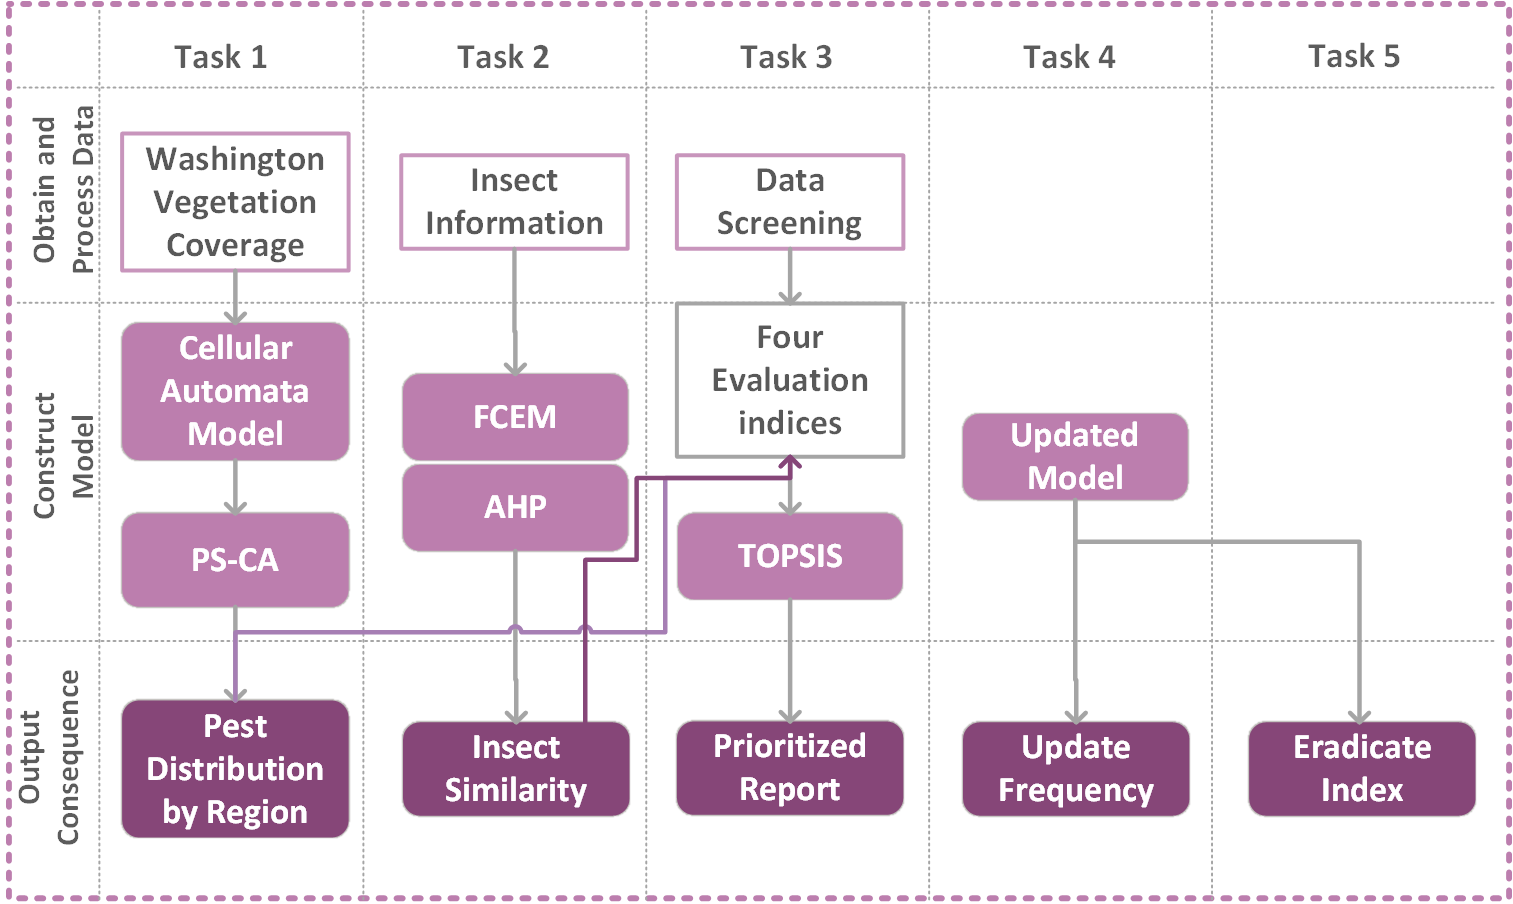
\includegraphics[scale = 0.45]{Chapter-2021C/images-2021C/workflow.png}
    \caption{Our Workflow.}
    \label{fig:workflow}
\end{figure}
\begin{itemize}                %%以圆点方式给出各点
    \item In task 1, we fully understand the reproduction characteristics and living habits of pests, consider the geographical factors of Washington State, decide to apply cellular automata to simulate the distribution of pests over time, and visualize the results on the map. Finally, we further test the model and analyze that the accuracy of the model is a $150m \times 150m$ area.
    \item For task 2, we try to build a similarity database according to the similarity of other types of insects and pest  from a visual perspective. In the paper, we select nine other types of insects and compare their characteristics to pest based on FCEM in terms of size, abdomen, head, chest, and nest. Then we use AHP to analyze the weight of each feature. Finally, the possibility of nine types of insects being misclassified is discussed from the visual similarity.
    \item As to task 3, we first use LR to filter the report to remove invalid reports with little information. Then we determine four indices to measure the accuracy of the report and use TOPSIS to score each report to obtain the ranking results. The four indices are the probability of occurrence, time activeness, note effectiveness and possibility of misclassification.
    \item As for task 4, we make efforts to optimize our model and clarify the update frequency. Starting from the perspective of multi-point invasion of pest, the new accurate sighting location is set as a new starting point in the PS-CA model, While destroy of pest nest is set as clearing an existing point. From the perspective of human intervention to prevent and control pests, we adjust the growth curve of pest every year to achieve reasonable simulation results.
    \item In terms of task 5, we set an index for the degree of eradication based on the optimized model. Then we run the PS-CA model to calculate the intervention period until the degree satisfy the criteria. In addition, we also conduct a sensitivity analysis of the model and achieve ideal results.
\end{itemize}

\section{Spread Simulation and Prediction}
In this section, we build pest's population migration model based on its special population characteristics and predict its distribution over time. We utilize the \textbf{Cellular Automata (CA)} to simulate the spread of pest and establish transition rule based on population migration characteristics. We name our model as \textbf{Pest Spread-Cellular Automata(PS-CA)} model. Finally we get the distribution map of pests spread over time, analyze the spread situation and study the precision of our model.%等到扩充

%%第一部分 建模
\subsection{Spread Simulation Preparations based on Cellular Automata}
Cellular Automata (CA) is an array of finite automata connected locally, which update their states in discrete time and at the same moments; every automaton updates its next state depending on the states of its closest neighbors \parencite{CA}. For example, Huynh, HX and his collegues have studied the spread of brown plant hoppers based on cellular automata \parencite{CAtheorem}. Similarly in this problem, we are going to predict the population migration of vespa mandarinia on the basis of cellular automata.

In the manner of formal language, cellular automata can be discribed as a 4-tuples:

\begin{equation*}
    \text{CA} = (L^d, S, N, f)
\end{equation*}
where CA is the cellular automata system, $L$ represents a regularly divided grid space, and each grid space is a cell, $d$ is the dimension of $L$, $S$ is a discrete finite set, $N$ symbolizes the neighbour set of cellular and $f$ is the transition rule.

To be specific, for each $N \subset L$, let the number of cells in the neighbor set be denoted as $n$, then $N$ can be interpreted as a combination of cells in a domain, that is, a space vector containing $n$ different cell states. Recorded as:

\begin{equation*}
    N = (s_1, s_2, \dots, s_n), s_i \in L, i \in (1, \dots, n)
\end{equation*}

Meanwhile, $f$ implies a mapping function: $S^n_t \xrightarrow{} S_{t+1}$. In other words, the state value of the cell at $t+1$ moment is determined by all the neighbours' state at $t$ moment. We will analyze it in detail in the next part.

After understanding the theorem of CA, we need to contruct a cellular automata model that fits the spread of pest, and the most important part is transition rule. In the beginning, let us make some bold assumptions:

\begin{itemize}
    \item \textbf{Natural enemies of pest are ignored.} Since the natural enemies of Vespa mandarinia have little effect on its containment and the types of natural enemies are too complex, we ignore this factor.
    \item \textbf{Its growth curve conforms to the J-curve.} When the foreign organisms invade, their survival pressure is at a low level, so the initial growth will be J-shaped. Our problem situation is exactly when the pests broke out rapidly in the early stage, so we can assume that its growth mode is J-type, except for its hibernation.%最好找到参考文献
    \item \textbf{The hibernation period of pests is from January to April.} When we observe the time of sighting of positve events, we find that they all occur from May to December, and this assumption is consistent with the pest’s living habits due to temperature changes.
\end{itemize}

On the basis of the former assumptions, our model construction and variable definition are accomplished through the following steps:

\begin{enumerate}[\quad\bf Step1.]
%%1
\item
We define the simulation area of Washington State. In order to include as more positive reports as possible, we define the simulation area from $123.9254^{\circ} W$ to $120.7114^{\circ} W$ in longitude and from $47.7294^{\circ} N$ to $49.1550^{\circ} N$ in latitude. The selected area is shown in Figure \ref{fig:2021C-The selected simulation area.} and it is also used in step 6 for our initialization.

In our model, we simply regard our simulation area as a rectangle and divide it into a lot of small ones, which represent a cell in our cellular automata model.

% The selected area is shown in Figure \ref{fig:2021C-The selected simulation area.}, and it is also used in step 6 to classify the geographical environment value, which is shown in Figure \ref{fig:2021C-Classification of geographical environment value.}.

%%2
\item
We denote a few notations in Table \ref{tbl:2021C-Notations of cellular automata}, including all the variable we use in our model.
%%三线表 cellular automata notation
\begin{table}[H]
    \renewcommand\arraystretch{2}   %%控制行间距
    \centering
    \caption{Notations of cellular automata.}
    \begin{tabular}{ccc}    %%三列均左对齐
        \toprule  %%表格横线加粗
        \specialrule{0em}{2pt}{2pt}    %%添加透明线控制行高
        Symbol & Definition & Notes \\
        \specialrule{0em}{2pt}{2pt}    %%添加透明线控制行高
        \midrule
        \specialrule{0em}{1pt}{1pt}
        $A$ & the set of n areas in the simulation area & $A = \{ a_1, a_2, \dots, a_n \}$ \\
        $X$ & the set of horizontal coordinates & $X = \{ x_1, x_2, \dots, x_n \}$ \\
        $Y$ & the set of vertical coordinates & $Y = \{ y_1, y_2, \dots, y_n \}$ \\
        $GE$ & the set of geographical environment & $GE = \{ ge_1, ge_2, \dots, ge_n \}$ \\
        $P$ & the set of pest with an ideal population growth & $P = \{ p_{1,t}, p_{2,t}, \dots, p_{n,t} \}$ \\
        $M$ & the set of migration & $M= \{ m_{1,t}, m_{2,t}, \dots, m_{n,t} \}$ \\
        $V^c$ & the set of current volume of pest & $V^c = \{ v^c_{1,t}, v^c_{2,t}, \dots v^c_{n,t}$ \} \\
        $S$ & the state of the cell & $S = \{ s_{1,t}, s_{2,t}, \dots, s_{n,t}$ \}\\
        $d_{max,t}$ & The maximum distance of spread at time t &  \\
        % $c^s_t$ & the spread coefficient at time $t$  & \\
        
        \specialrule{0em}{1pt}{1pt}
        \bottomrule
    \end{tabular}
    \label{tbl:2021C-Notations of cellular automata}
\end{table}

Each cell represents an area, which is described by coordinate $x$ and $y$. Moreover, we also take other factors into consideration, such as the geographical environment $ge$, the population growth of pests $p_{i,t}$ and the current volume $v^e_{i,t}$. Now we get the cellular automata model as follows:

\begin{equation*}
    A = L^6 = (X \times Y \times GE \times P \times M\times V^c),
\end{equation*}
% where $A_i$ at the time $t$ is presented by $(x_i,y_i,ge_i,m_i,v^c_{1,t})$
where $a_i$ at the time $t$ is presented by $(x_i, y_i, ge_i, p_{i,t},m_{i,t},v^c_{i,t})^T$.


%%3
\item
We clarify the meaning of the cell state. Each cell is assigned a state at a time and it describes the degree of the pest gathering, which can imply the likelihood that the citizen in this area report to discover Asian giant hornets. At a specific time $t$, we simply let the current volume $v^c_{i,t}$ be the state of an area $s_{i,t}$, so that $s_{i,t} = v^c_{i,t}$ can be displayed directly the possibility of pest occurrence.

%%4
\item
We determine the neighborhood vector by using the Moore neighborhood method. Through this method, the central cell is related to its eight surrounding cells like Figure \ref{fig:2021C-The Moore neighborhood method.}.

%%图片 Moore neighborhood method
\begin{figure}[H]
    \centering
    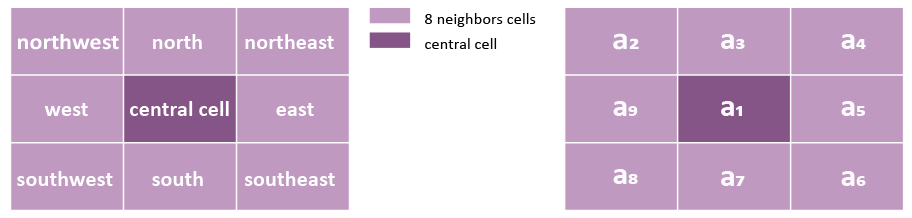
\includegraphics[scale = 0.4]{Chapter-2021C/images-2021C/1-mooer.png}
    \caption{The Moore neighborhood method.}
    \label{fig:2021C-The Moore neighborhood method.}
\end{figure}

For the central cell, its neighbors are presented by a set N with $$N = \{a_2, a_3, a_4, a_5, a_6, a_7, a_8, a_9\}$$ Next, we will use this subscript variable to do a small calculation description.

%%5
\item
Next, We consider the transition rule of the current volume $v^c_{i,t}$.

According to the living habits of the pests that they actively appears in months from May to December when the queen start to build new nest and reproduce. Therefore, we stop simulation from January to April and restart it at the beginning of May.

As for the $i^{th}$ area, the current volume at $t+1$ moment $v^c_{i,t+1}$ depends on the number of pest population growth at $t$ moment $p_{i,t}$ and the number of migration at $t+1$ moment.
For clarity, we only calculate and explain within the range of Moore  neighborhood, that is, $i= 1,2,\dots,9$.
According to the J-curve, we know that 
    $$p_{i,t} = N_0 \times \lambda^t$$ 
where $N_0$ and $\lambda$ are constant, and
    $$\frac{p_{i,t+1}}{p_{i,t}} = \frac{N_0 \times \lambda^{t+1}}{N_0 \times \lambda^t} = \lambda$$ 
Then we have  $$p_{i,t+1} = \lambda \times p_{i,t}$$
We define the number of pest migration in central cell as depending on its current volume and the geographical environment of its eight neighbors.
    \begin{equation*}
        \label{equ:transition rule}
        m_{1,t} = \frac{ge_k}{ge_k+4} \times v^c_{1,t}, 
    \end{equation*}
where $ge_k = max \{ ge_i \} (i=2, 3, \dots, 9)$ is the maximum of the $ge$ of the neighbor cells.
In all, we achieve the transition rule that is 
    $$v^c_{1,t+1} = \lambda \times p_{1,t} + m_{1,t}.$$
\vspace{-0.6cm}
%%6
\item
We initialize the value of the geographical environment set $GE$ as Figure \ref{fig:2021C-Process of GE.} shows and the starting point. Then we search and get the simulation area map according to Figure \ref{fig:2021C-The selected simulation area.} and the legend in it\parencite{GoogleMap}. The figure shows the vegetation coverage of this area.

The pest typically build their nests underground, usually in abandoned
rodent burrows in forests\parencite{attachment}. So we infer that pest is more likely to migrate to places with lush vegetation. We classify the value of $ge_i$ for each cell according to the difference of vegetation coverage in Figure \ref{fig:2021C-Classification of GE.}. In detail, we allocate rivers and regions with no vegetation coverage with value 0. Additionally, we grant the value of 4, 3, and 1 to the areas with the green colour from deep to shallow. The result can be seen in Figure \ref{fig:2021C-Value Allocation of GE.}. In conclusion, the bigger the value of $ge_i$ is, the more likely it is for the pests to migrate to this area.

% \begin{figure}[H] 
% \begin{minipage}[t]{0.5\linewidth} 
% \centering 
% 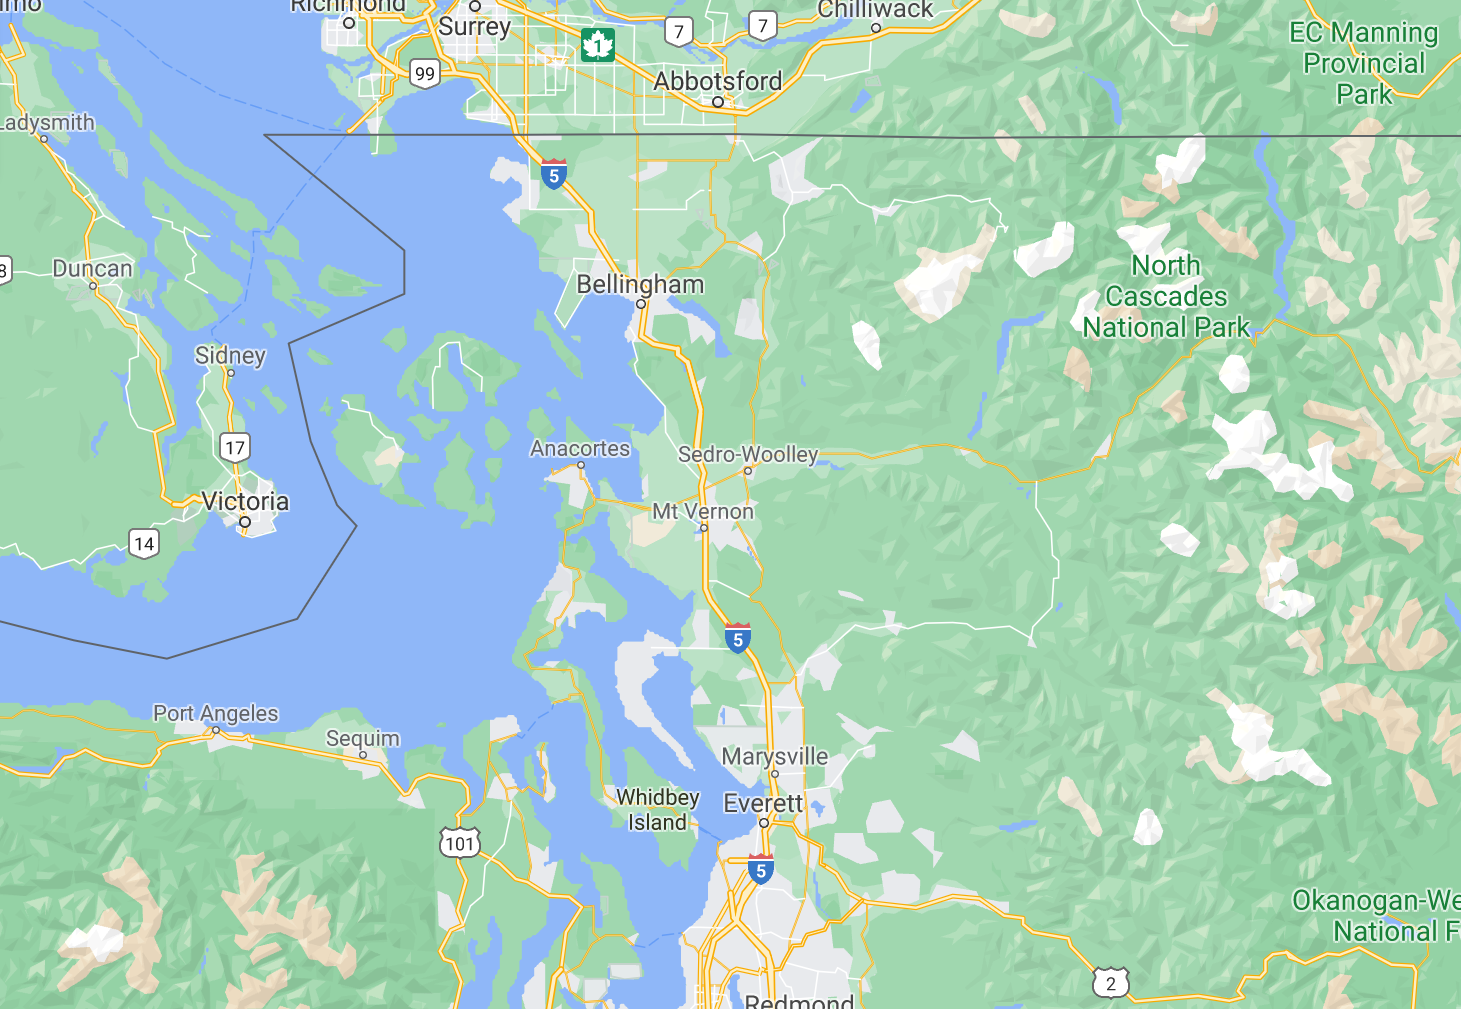
\includegraphics[width=2.5in]{Chapter-2021C/images-2021C/1-map.png} 
% \caption{The selected simulation area.} 
% \label{fig:2021C-The selected simulation area.} 
% \end{minipage}
% \begin{minipage}[t]{0.5\linewidth} 
% \centering 
% 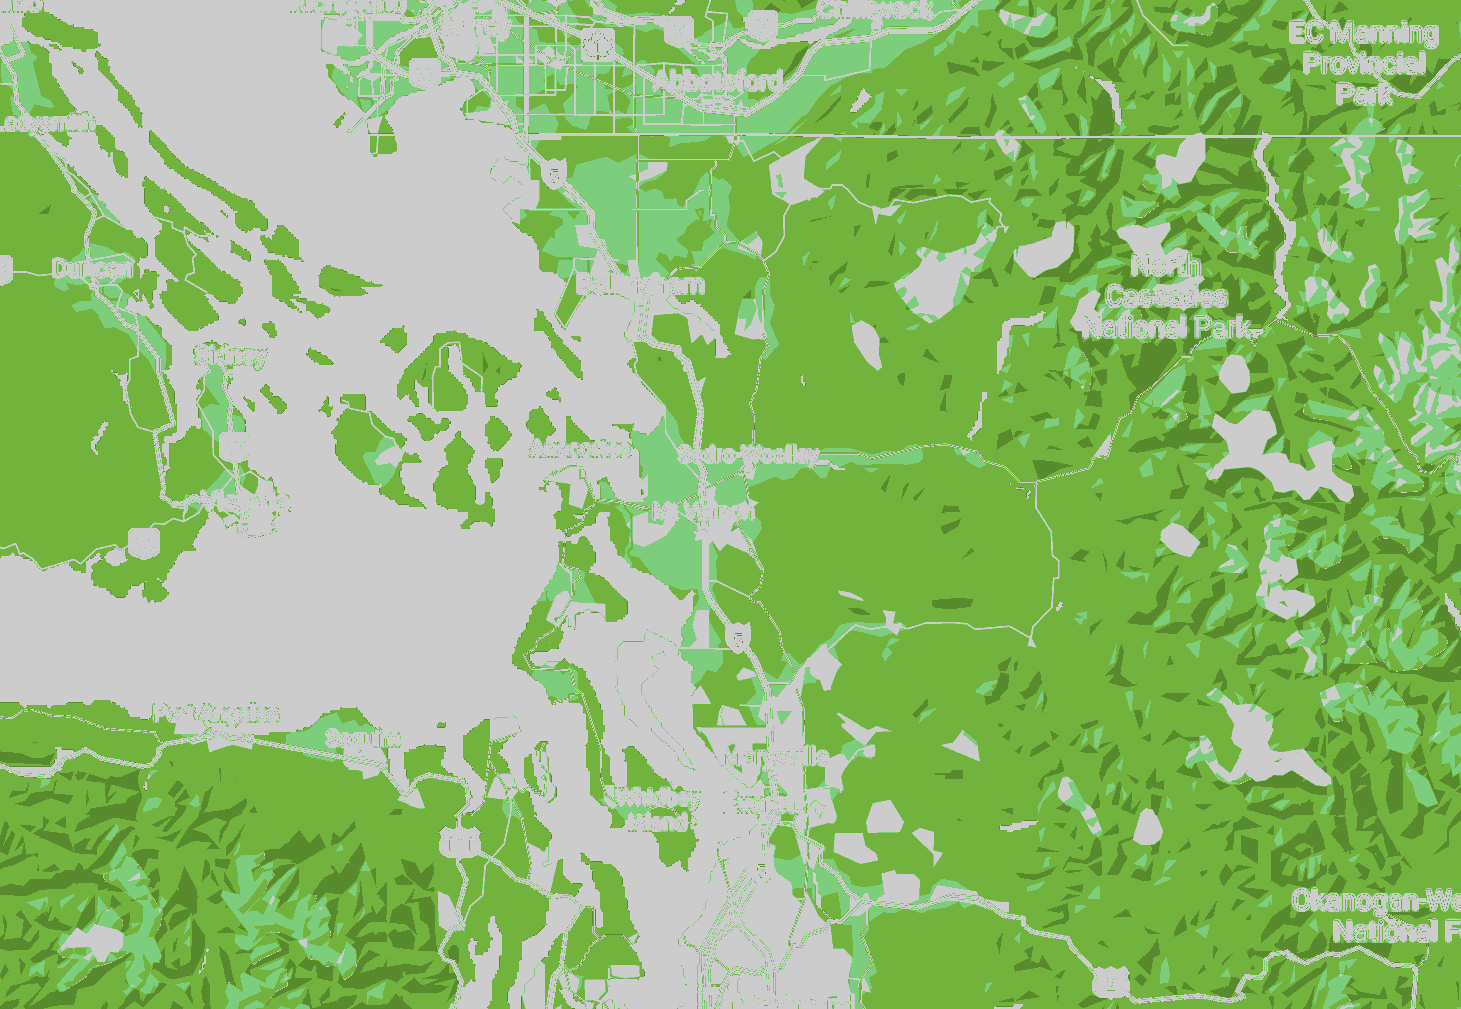
\includegraphics[width=2.5in]{Chapter-2021C/images-2021C/1-classification.png} 
% \caption{Classification of $GE$.} 
% \label{fig:2021C-Classification of GE.} 
% \end{minipage} 
% \end{figure}

\begin{figure}[H]
\centering
\subfigure[Simulation area.]{
\begin{minipage}[t]{0.33\linewidth}
\centering
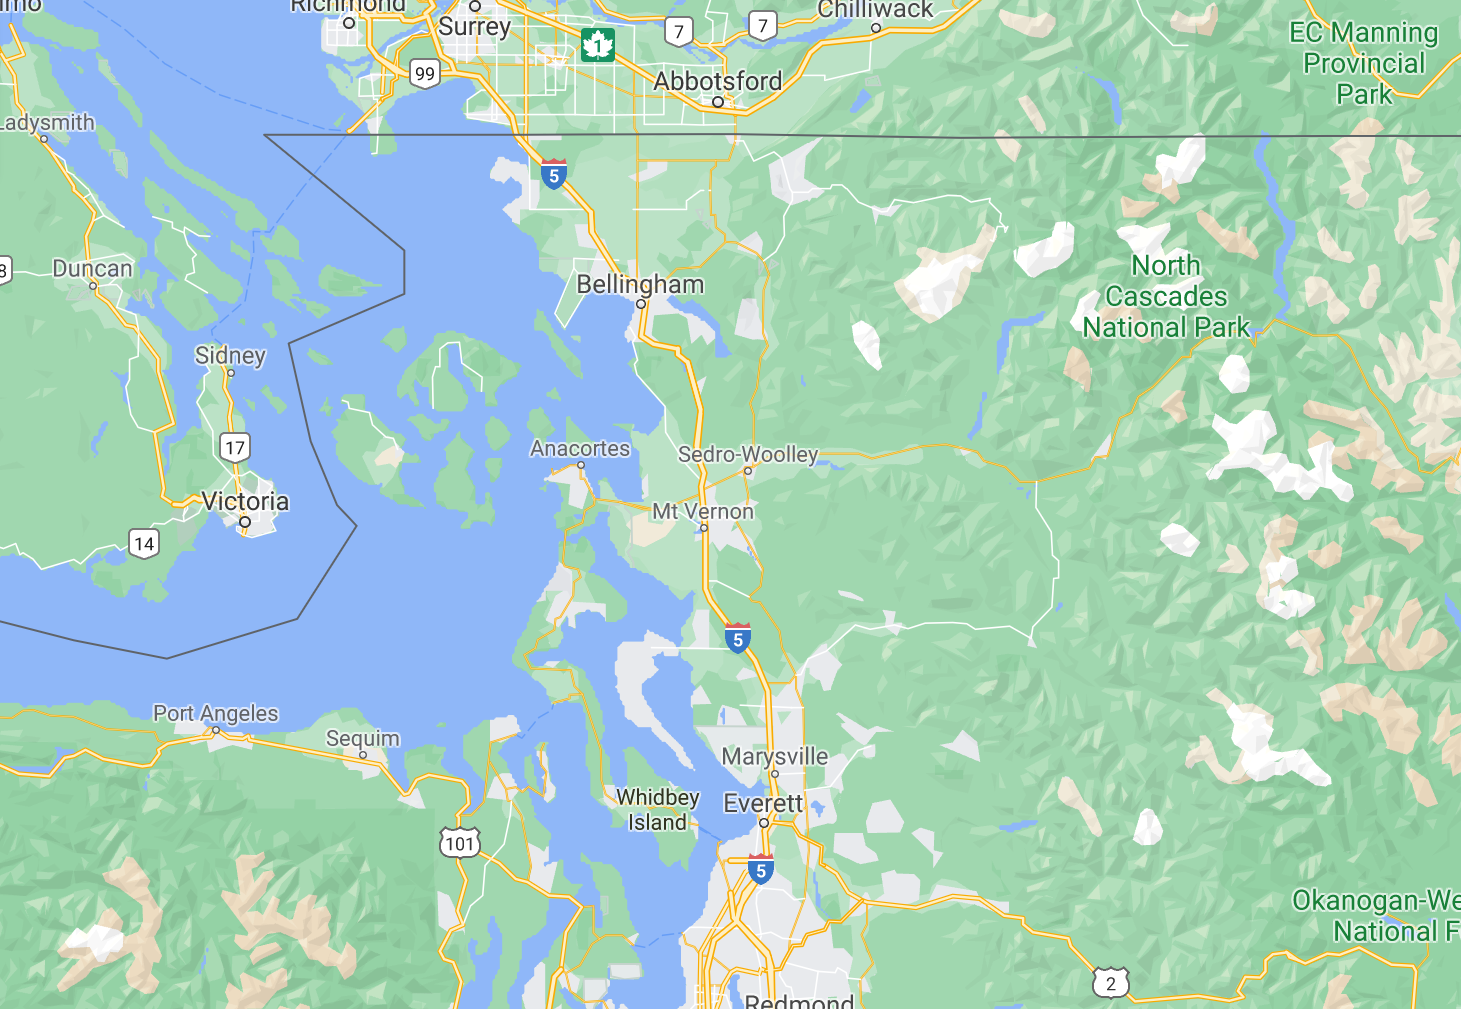
\includegraphics[width=1.7in]{Chapter-2021C/images-2021C/1-map.png}
%\caption{fig1}
\label{fig:2021C-The selected simulation area.} 
\end{minipage}%
}%
\subfigure[Classification of $GE$.]{
\begin{minipage}[t]{0.33\linewidth}
\centering
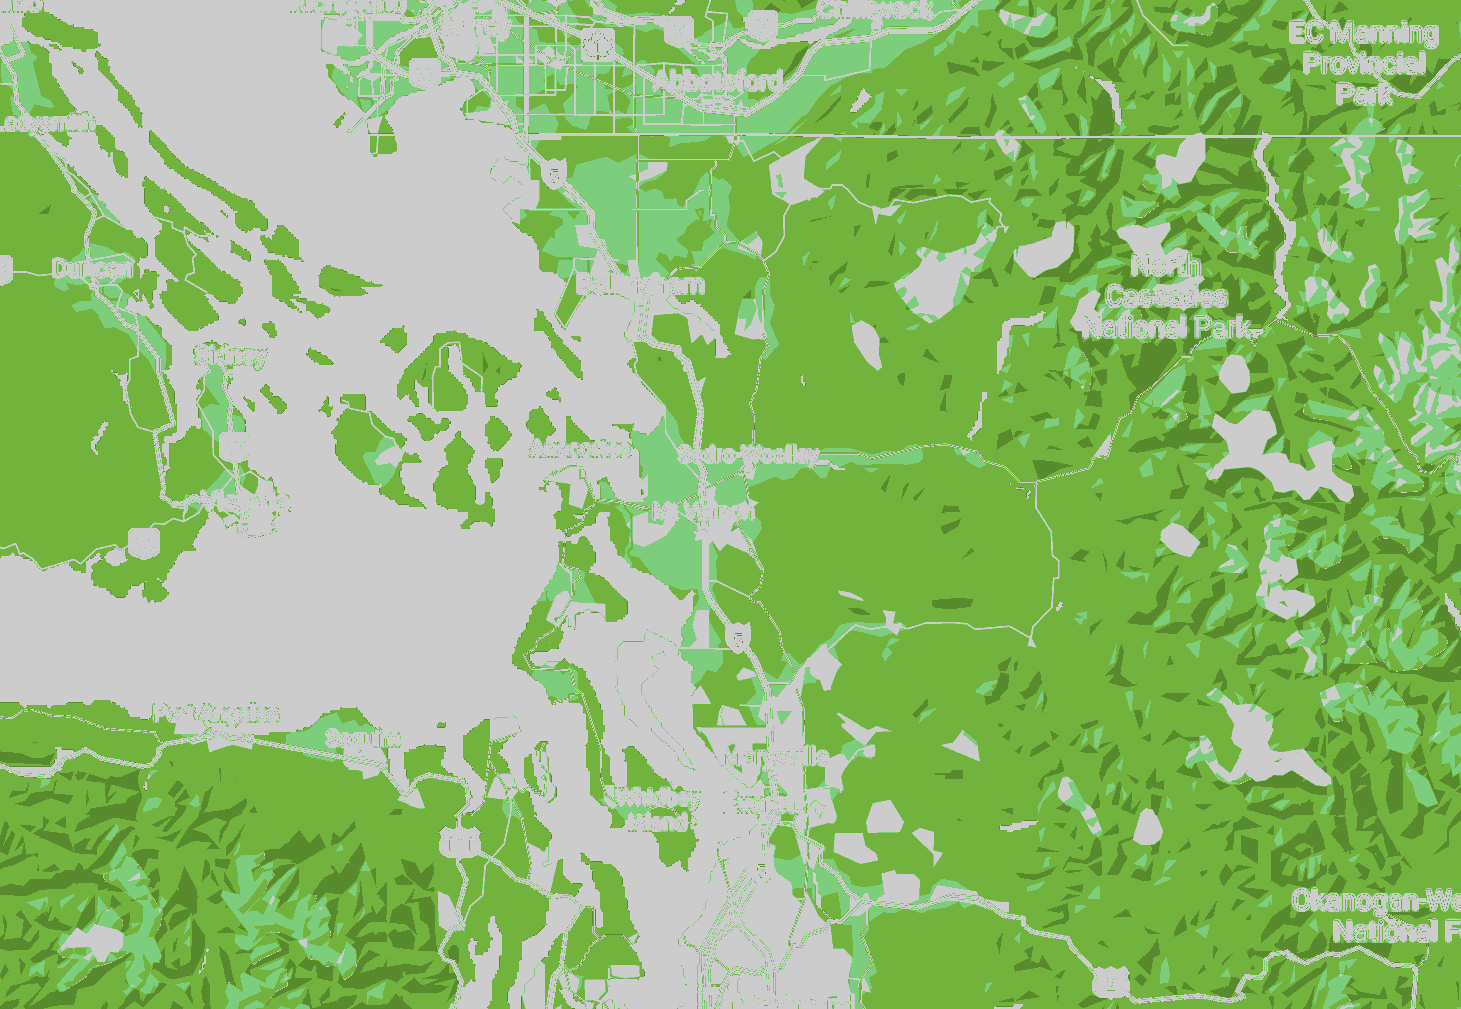
\includegraphics[width=1.7in]{Chapter-2021C/images-2021C/1-classification.png}
%\caption{fig2}
\label{fig:2021C-Classification of GE.} 
\end{minipage}%
}%
\subfigure[Value Allocation of GE.]{
\begin{minipage}[t]{0.33\linewidth}
\centering
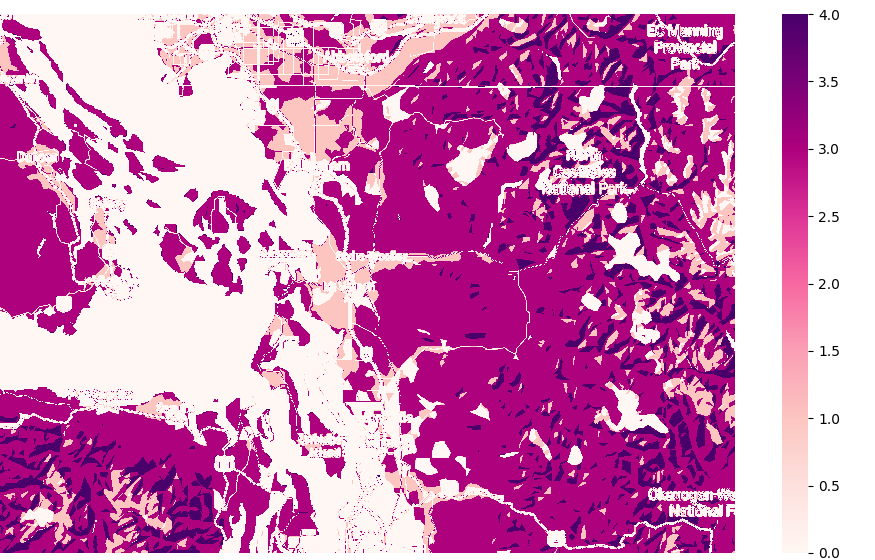
\includegraphics[width=1.9in]{Chapter-2021C/images-2021C/1-gescore.png}
%\caption{fig2}
\label{fig:2021C-Value Allocation of GE.} 
\end{minipage}
}%
\centering
\caption{Process of $GE$.}
\label{fig:2021C-Process of GE.} 
\end{figure}

\vspace{-0.5cm}

After that, we are ready to initialize the starting point and set the initial pest population $P_{i,1}$ and the value of constant $\lambda$. According to the detection time, the earliest positive report is at $(123.9431^{\circ}W , 49.149396^{\circ}N)$. However, the report place is far away from other ones and is blocked by a river. Additionally, no new positive reports emerge near it so that we ignore this report. Then we select the next report place $(122.7022^{\circ}W, 48.99389^{\circ}N)$ as the starting point on 2019/9/30. Moreover, we set the initial pest population $p_{start,1}$ as 200, the simulation time as 380 to include the detection time of the last positive report, and the constant $\lambda$ as $1.2$.

\end{enumerate}

\subsection{Spread Simulation Consequence}
After the above steps of preparation and initialization, we run the cellular automata. Then we get the simulation consequence of one year as Figure \ref{fig:2021C-Simulation of pest spread in one year.} shows and the one of two years as Figure \ref{fig:2021C-Simulation of pest spread in two years.} shows.

% \begin{figure}[H] 
% \begin{minipage}[t]{0.25\linewidth} 
% \centering 
% 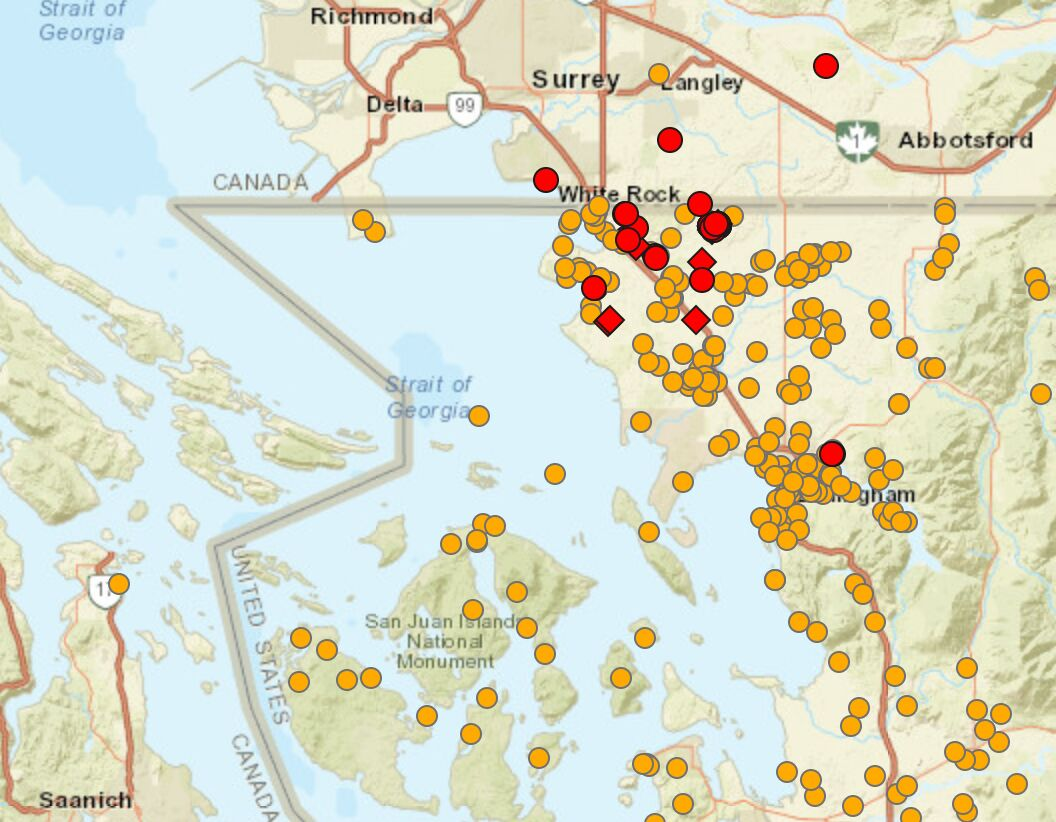
\includegraphics[width=1in]{Chapter-2021C/images-2021C/1-positive reality.jpg}
% \caption{Reality of positive reports.} 
% \label{fig:2021C-Reality of positive reports.} 
% \end{minipage}
% \begin{minipage}[t]{0.25\linewidth} 
% \centering 
% 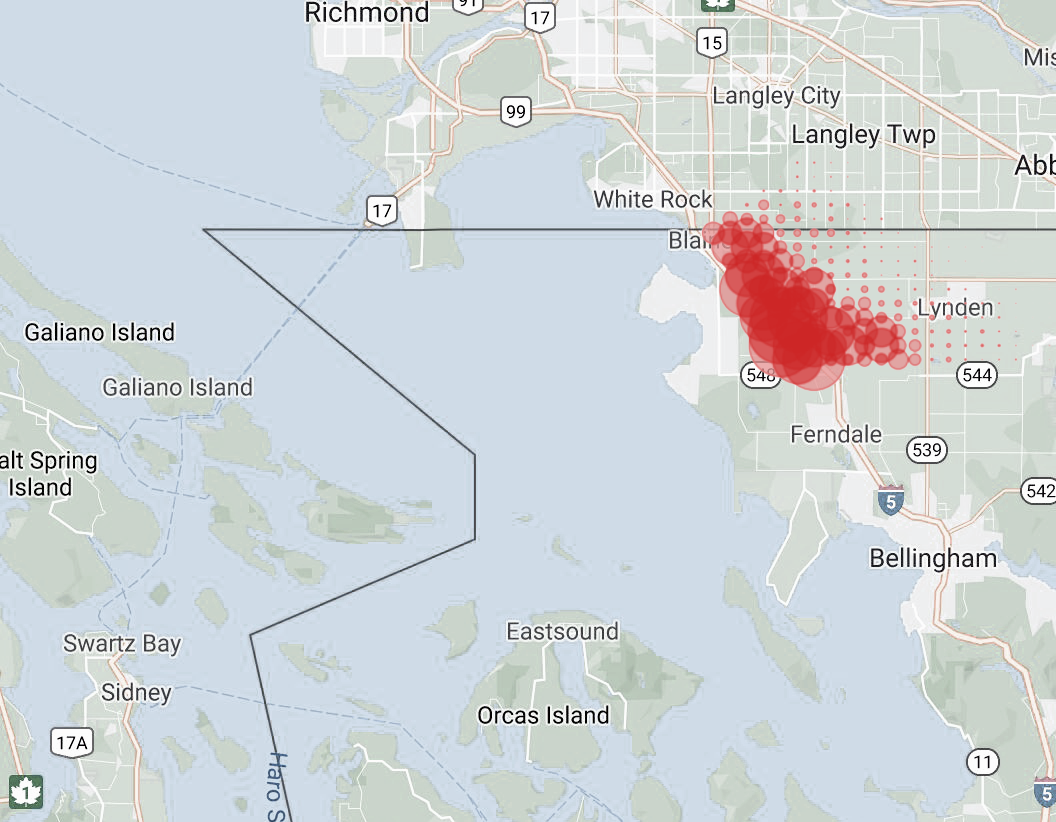
\includegraphics[width=1in]{Chapter-2021C/images-2021C/1-positive simulation.png} 
% \caption{Simulation of pest spread in one year.} 
% \label{fig:2021C-Simulation of pest spread in one year.} 
% \end{minipage} 
% \begin{minipage}[t]{0.25\linewidth} 
% \centering 
% 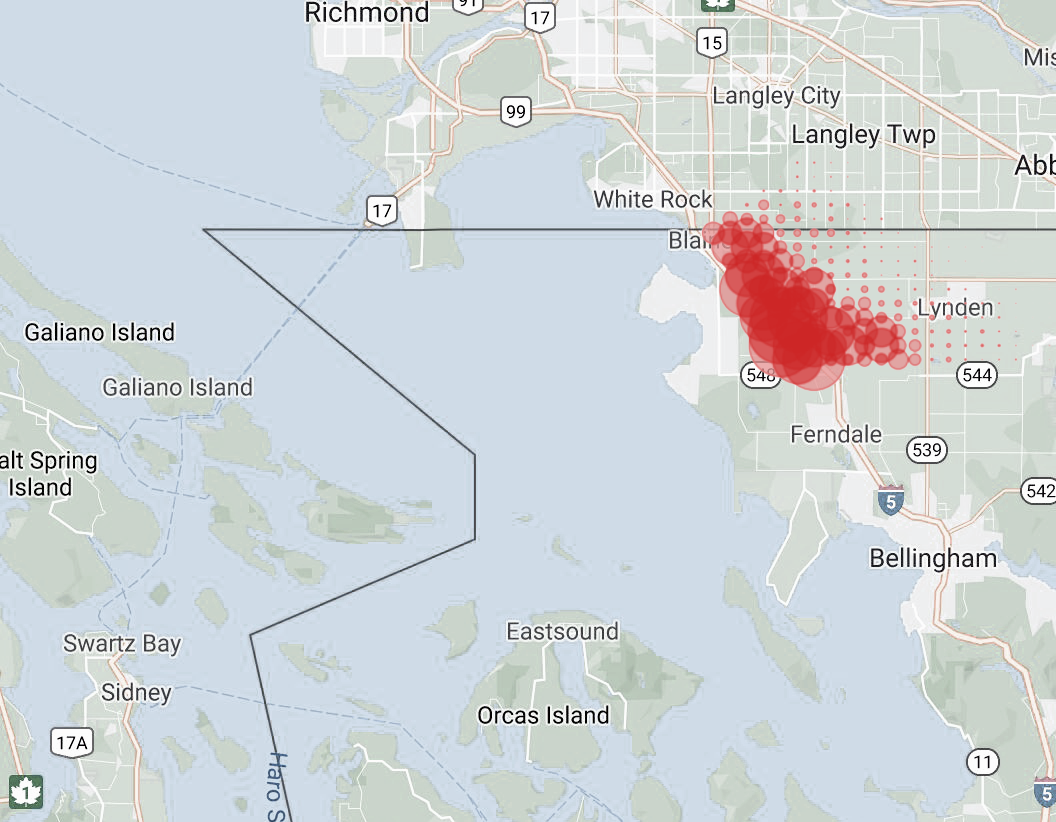
\includegraphics[width=1in]{Chapter-2021C/images-2021C/1-positive simulation.png} 
% \caption{Simulation of pest spread in two years.} 
% \label{fig:2021C-Simulation of pest spread in two years.} 
% \end{minipage} 
% \end{figure}

\begin{figure}[H]
\centering
\subfigure[Reality of positive reports.]{
\begin{minipage}[t]{0.33\linewidth}
\centering
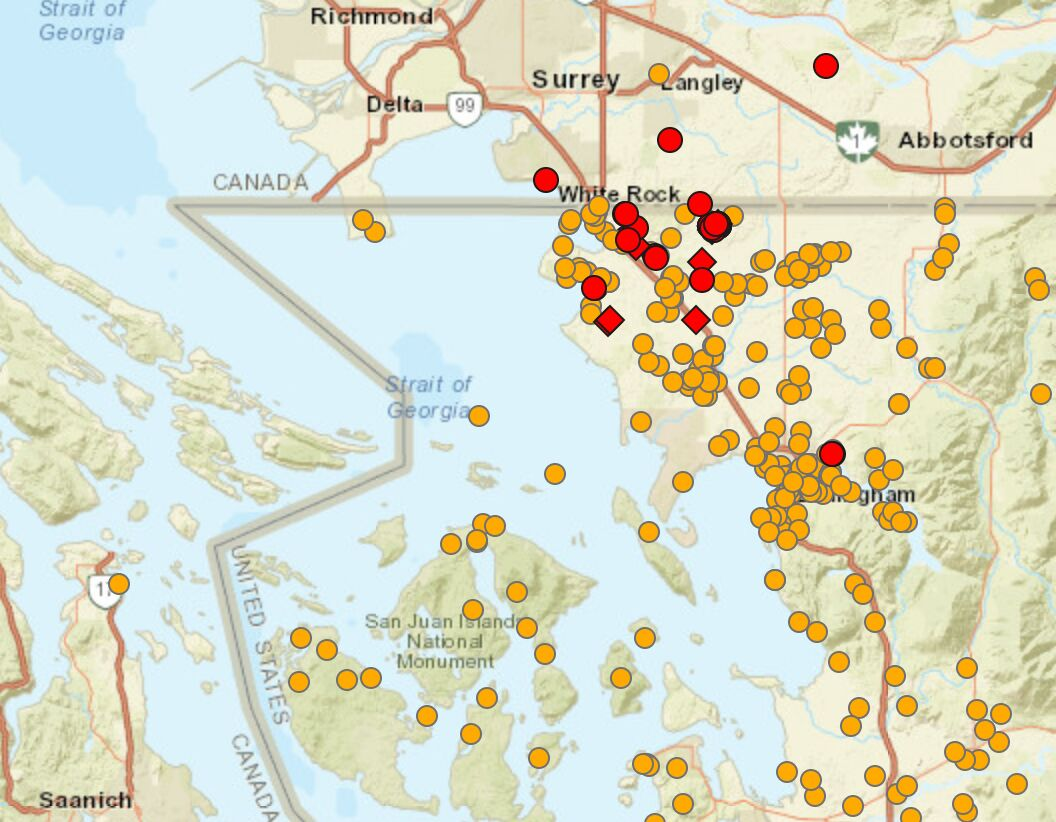
\includegraphics[width=1.7in]{Chapter-2021C/images-2021C/1-positive reality.jpg}
%\caption{fig1}
\label{fig:2021C-Reality of positive reports.} 
\end{minipage}%
}%
\subfigure[Simulation of one year.]{
\begin{minipage}[t]{0.33\linewidth}
\centering
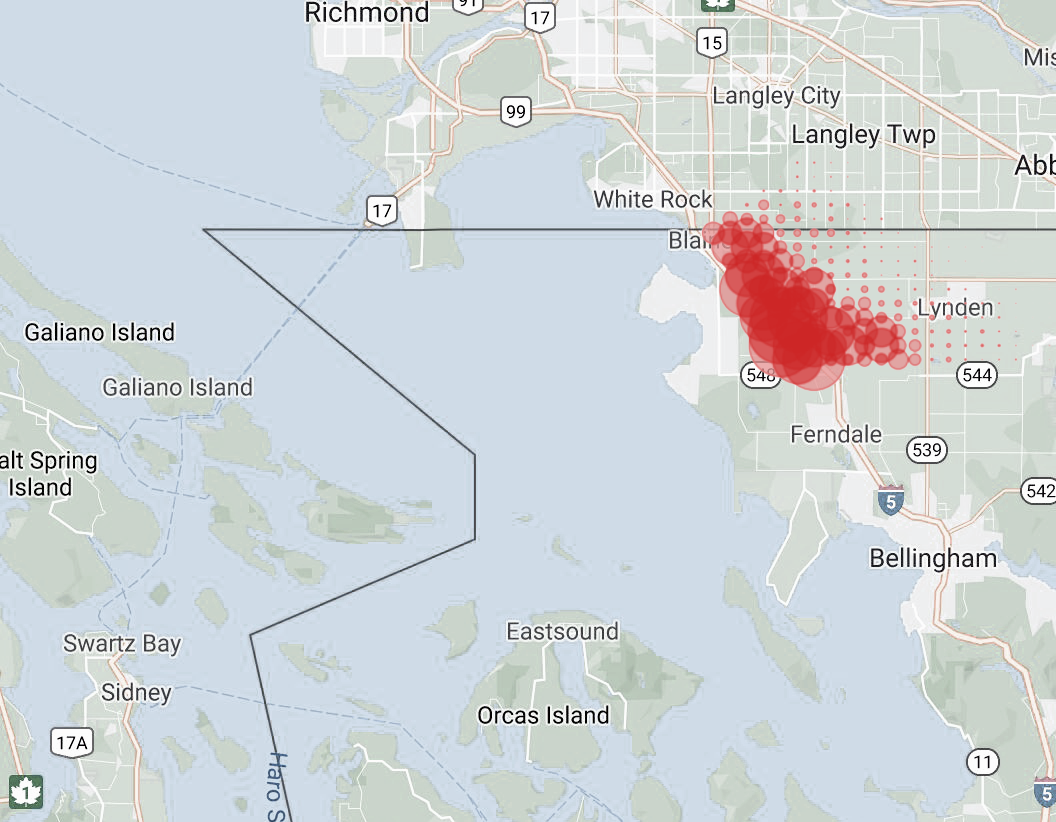
\includegraphics[width=1.7in]{Chapter-2021C/images-2021C/1-positive simulation.png}
%\caption{fig2}
\label{fig:2021C-Simulation of pest spread in one year.} 
\end{minipage}%
}%
\subfigure[Simulation of two years.]{
\begin{minipage}[t]{0.33\linewidth}
\centering
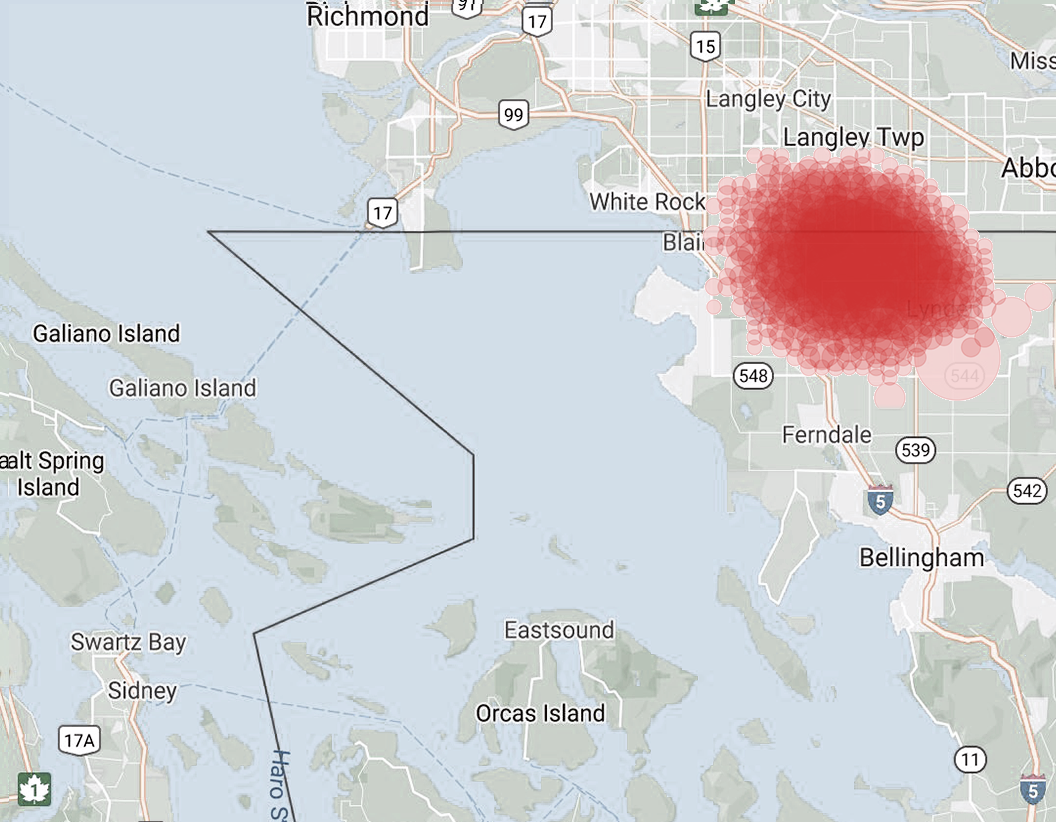
\includegraphics[width=1.7in]{Chapter-2021C/images-2021C/1-positive simulation2.png}
%\caption{fig2}
\label{fig:2021C-Simulation of pest spread in two years.} 
\end{minipage}
}%
\centering
\caption{Comparison of Reality and Simulation.}
\end{figure}

In Figure \ref{fig:2021C-Reality of positive reports.}, red points represent the real place of these positive reports. This figure was taken from the Asian Hornet dashboard published by the Washington State Department of Agriculture\parencite{Public-Dashboard}.

In Figure \ref{fig:2021C-Simulation of pest spread in one year.}, we can conclude that the spread of the pest is gathered in a relatively small region around the starting point. In addition, the spread of pest avoid the rivers, which is absolutely in line with our design.

In Figure \ref{fig:2021C-Simulation of pest spread in two years.}, the pest spread to a bigger region and the situation becomes more serious.

Comparing the two figures \ref{fig:2021C-Reality of positive reports.} and \ref{fig:2021C-Simulation of pest spread in one year.}, we have the similar spread region in one year and we want to make some further investigations.

To quantify the potential spread threat, we calculate the entire pest number by summing up all states of cells and propose it in Figure \ref{fig:2021C-The entire pest number.}. From the figure, we can see a relatively slow increasing during the first year and unchanged sum for four months, but a dramatic rocketing at the beginning of May next year. An initial nest of 200 pests can grow to a big This phenomenon indicates that the pest will meet an amazing boom in their reproduction time next year, which will pose huge threat to areas nearby.

%%插图 总数 和最远距离
%%图片 sum
\begin{figure}[H] 
\begin{minipage}[t]{0.5\linewidth} 
\centering 
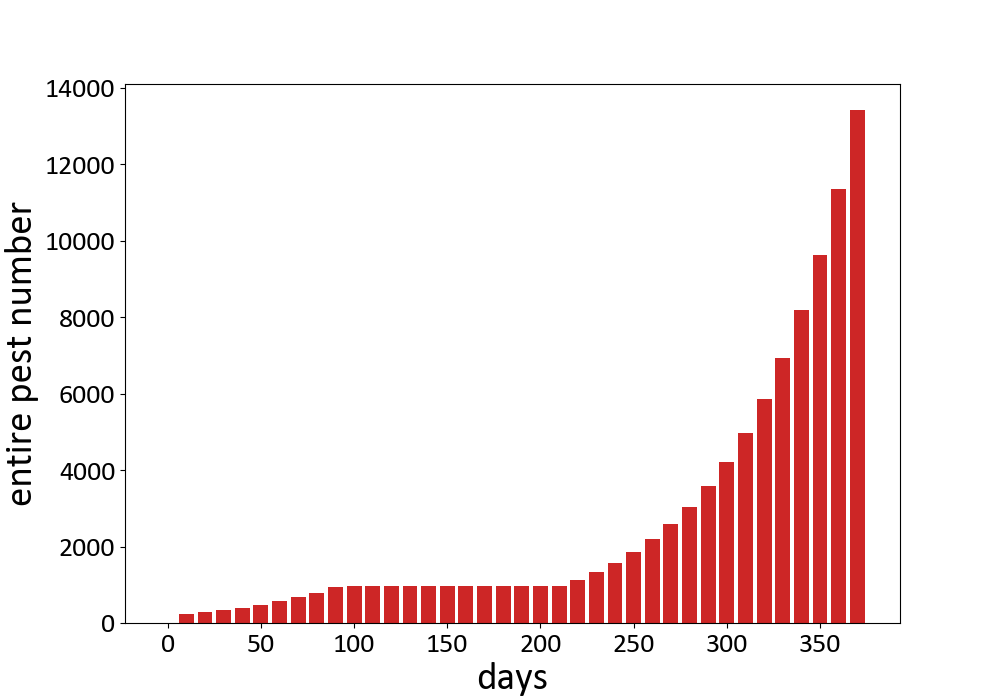
\includegraphics[width=2.5in]{Chapter-2021C/images-2021C/1-sum.png}
    \caption{The entire pest number.}
    \label{fig:2021C-The entire pest number.}
\end{minipage}
\begin{minipage}[t]{0.5\linewidth} 
\centering 
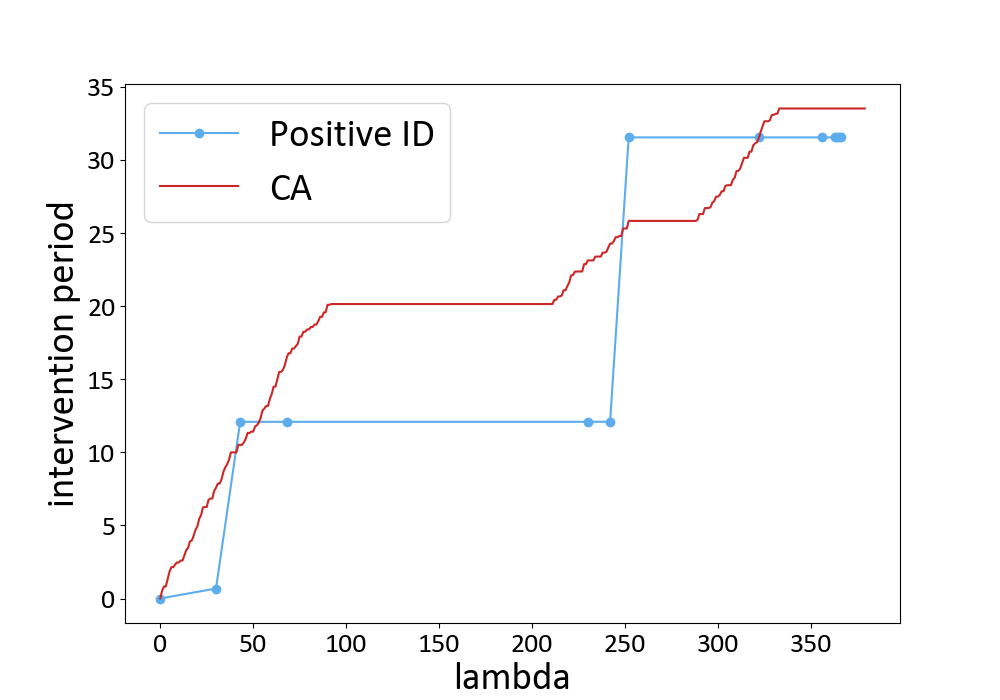
\includegraphics[width=2.5in]{Chapter-2021C/images-2021C/1-distance.png}
    \caption{The longest spread distance.}
    \label{fig:2021C-The longest spread distance.}
\end{minipage} 
\end{figure}

Moreover, we calculate the longest spread distance at each time $t$, convert the cell number to the distance in kilometer, and picture it in Figure \ref{fig:2021C-The longest spread distance.}. In this figure, we compare the longest spread distance of CA simulation with the one of positive reports. We notice that the longest spread distance of  CA simulation is always bigger than the other, which means the simulation have rationality in the reality. The spread can reach at most 34 km after the simulation of 380 days and remains to be a huge potential threat.

\subsection{Precision Analysis}
To do further test towards our simulation, we try to analyze the precision of our model. We incline to point out the place of the positive reports on the picture of the simulation until that day. We extract totally 12 positive reports except for the starting point and the ignored one. We select two of the 12 tests and propose it as followed in Figure \ref{fig:2021C-Positive reports on 2019/10/30.} and Figure \ref{fig:2021C-Positive reports on 2019/12/8.}, where the yellow area denotes our simulation area and the red triangle represents the place of the positive report on that day.

%%插图 标点精确度分析
\begin{figure}[H] 
\begin{minipage}[t]{0.5\linewidth} 
\centering 
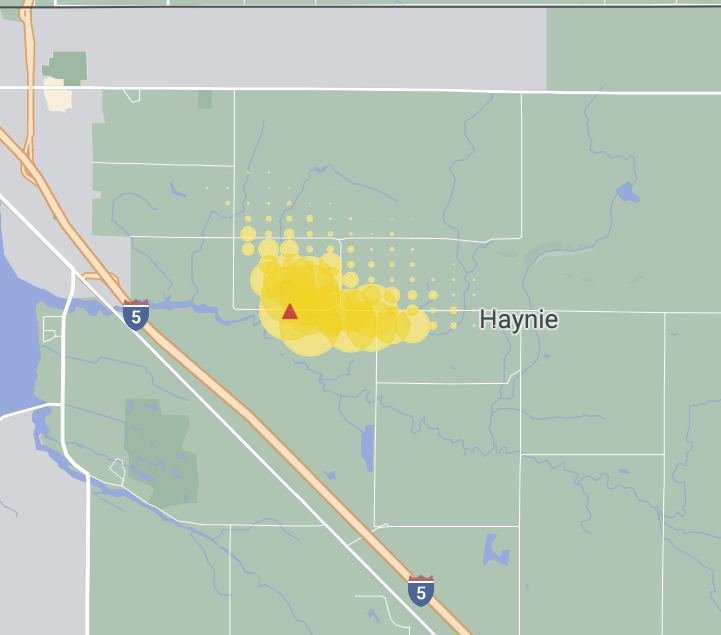
\includegraphics[width=2.2in]{Chapter-2021C/images-2021C/1-10-30.png} 
\caption{Positive reports on 2019/10/30.} 
\label{fig:2021C-Positive reports on 2019/10/30.} 
\end{minipage}
\begin{minipage}[t]{0.5\linewidth} 
\centering 
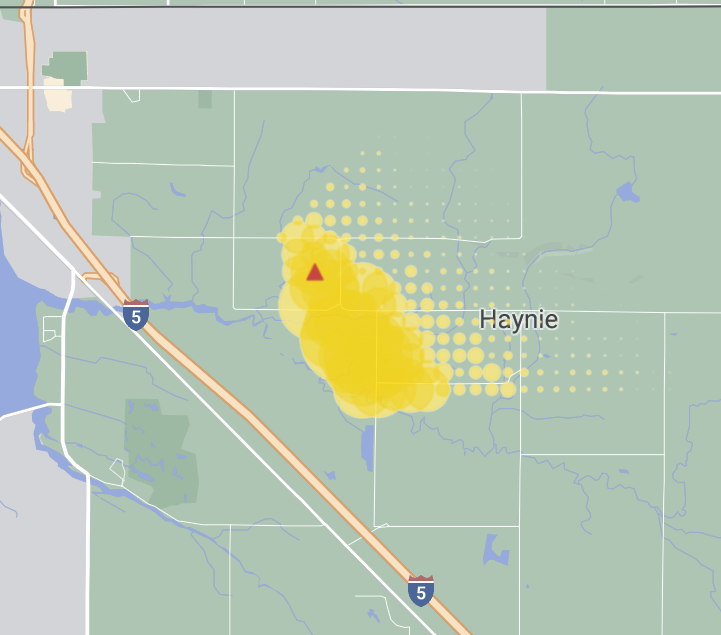
\includegraphics[width=2.2in]{Chapter-2021C/images-2021C/1-12-8.png} 
\caption{Positive reports on 2019/12/8.} 
\label{fig:2021C-Positive reports on 2019/12/8.} 
\end{minipage} 
\end{figure}

Considering all the 12 pictures, we can conclude that the positive reports are all located at the places with high current volumes in the simulation. In our model, we divide the longitude and the latitude into about 1500 and 1000 pieces, respectively. After transformation to meters, one piece of small rectangle represents 150m and 160m of width and length in the real life. So we can say confidently that our model achieves the precision of a $150m \times 150m$ area.

\vspace{1cm}

\section{Identification and Classification of Pest}
In this section, we cleverly combine \textbf{Fuzzy Comprehensive Evaluation Method (FCEM)} and \textbf{Analytic Hierarchy Process (AHP)} to construct a model distinguishing other types of insects from Asian giant hornets. Then we predict the likelihood of insects being misclassified based on the similarity between them.

\subsection{Create FCEM Model}
FCEM is a comprehensive evaluation strategy based on fuzzy mathematics. Our FCEM model contains the notations in Table \ref{tbl:2021C-Notations of FCEM}.

\begin{table}[H]
    \renewcommand\arraystretch{2}   %%控制行间距
    \centering
    \caption{Notations of FCEM.}
    \begin{tabular}{ccc}    %%三列均左对齐
        \toprule  %%表格横线加粗
        \specialrule{0em}{2pt}{2pt}    %%添加透明线控制行高
        Symbol & Definition & Notes \\
        \specialrule{0em}{2pt}{2pt}    %%添加透明线控制行高
        \midrule
        \specialrule{0em}{1pt}{1pt}
        $F$ & the set of $n$ evaluation factors & $F = \{ F_1, F_2, \dots, F_n \}$ \\
        $SP$ & the set of m samples & $SP = \{ sp_1, sp_2, \dots, sp_m \}$ \\
        $FV$ & the set of factor values of m samples & $FV = \{ FV^1, FV^2, \dots, FV^m \}$ \\
        $FV^i$ & the set of n factor values in sample $sp_i$ & $FV^i = \{ fv^i_1, fv^i_2, \dots, fv^i_n \}$ \\
        $W$ & the set of factor weights based on AHP & $W = \{ w_1, w_2, \dots, w_n \}$ \\
        $Value$ & the set of m sample values & $v = \{ v_1, v_2, \dots, v_m \}$ \\
        \specialrule{0em}{1pt}{1pt}
        \bottomrule
    \end{tabular}
    \label{tbl:2021C-Notations of FCEM}
\end{table}

For a better example, we choose entirely 9 types of insects, 5 detailed insects from the attachment of PennState Extention\parencite{attachment} and other 4 that appear most frequently in Lab Comment.

For each sample $sp_i$ in the sample set $SP$, we get its value $v_i$ by FCEM through the following equation.

\begin{equation*}
    v_i = \sum_{j=0}^n fv^i_j \times w_j\quad (i = 1, 2, \dots, m),
\end{equation*}
where $fv^i_j$ is defined and valued by FCEM and $w_j$ is allocated by AHP in the next part. The value is used to indicate the similarity between the insect sample and the pest, in other words the likelihood of the mistaken classification.

\subsection{Analyze Factor and Distribute Weight for AHP}
Firstly, we propose five factors on the reference of the introduction, including the \textbf{size}, \textbf{abdomen}, \textbf{head}, \textbf{chest}, and \textbf{nest}.

Secondly, we collect the factor features of all types of insects in aspects of the above factors. For example, the pest is 1.5 inches long and have abdomen banded with yellow and black and black chest. Additionally, the pests' nests are built in the dead, hollow trunks or roots of trees that are never more than 3 to 6 feet above the ground \parencite{attachment}. We look for information and draw the ten bees in Figure \ref{fig:2021C-Factor features of different bees.} to vividly show the difference between them, including size, colour and so on.

\begin{figure}[H]
    \centering
    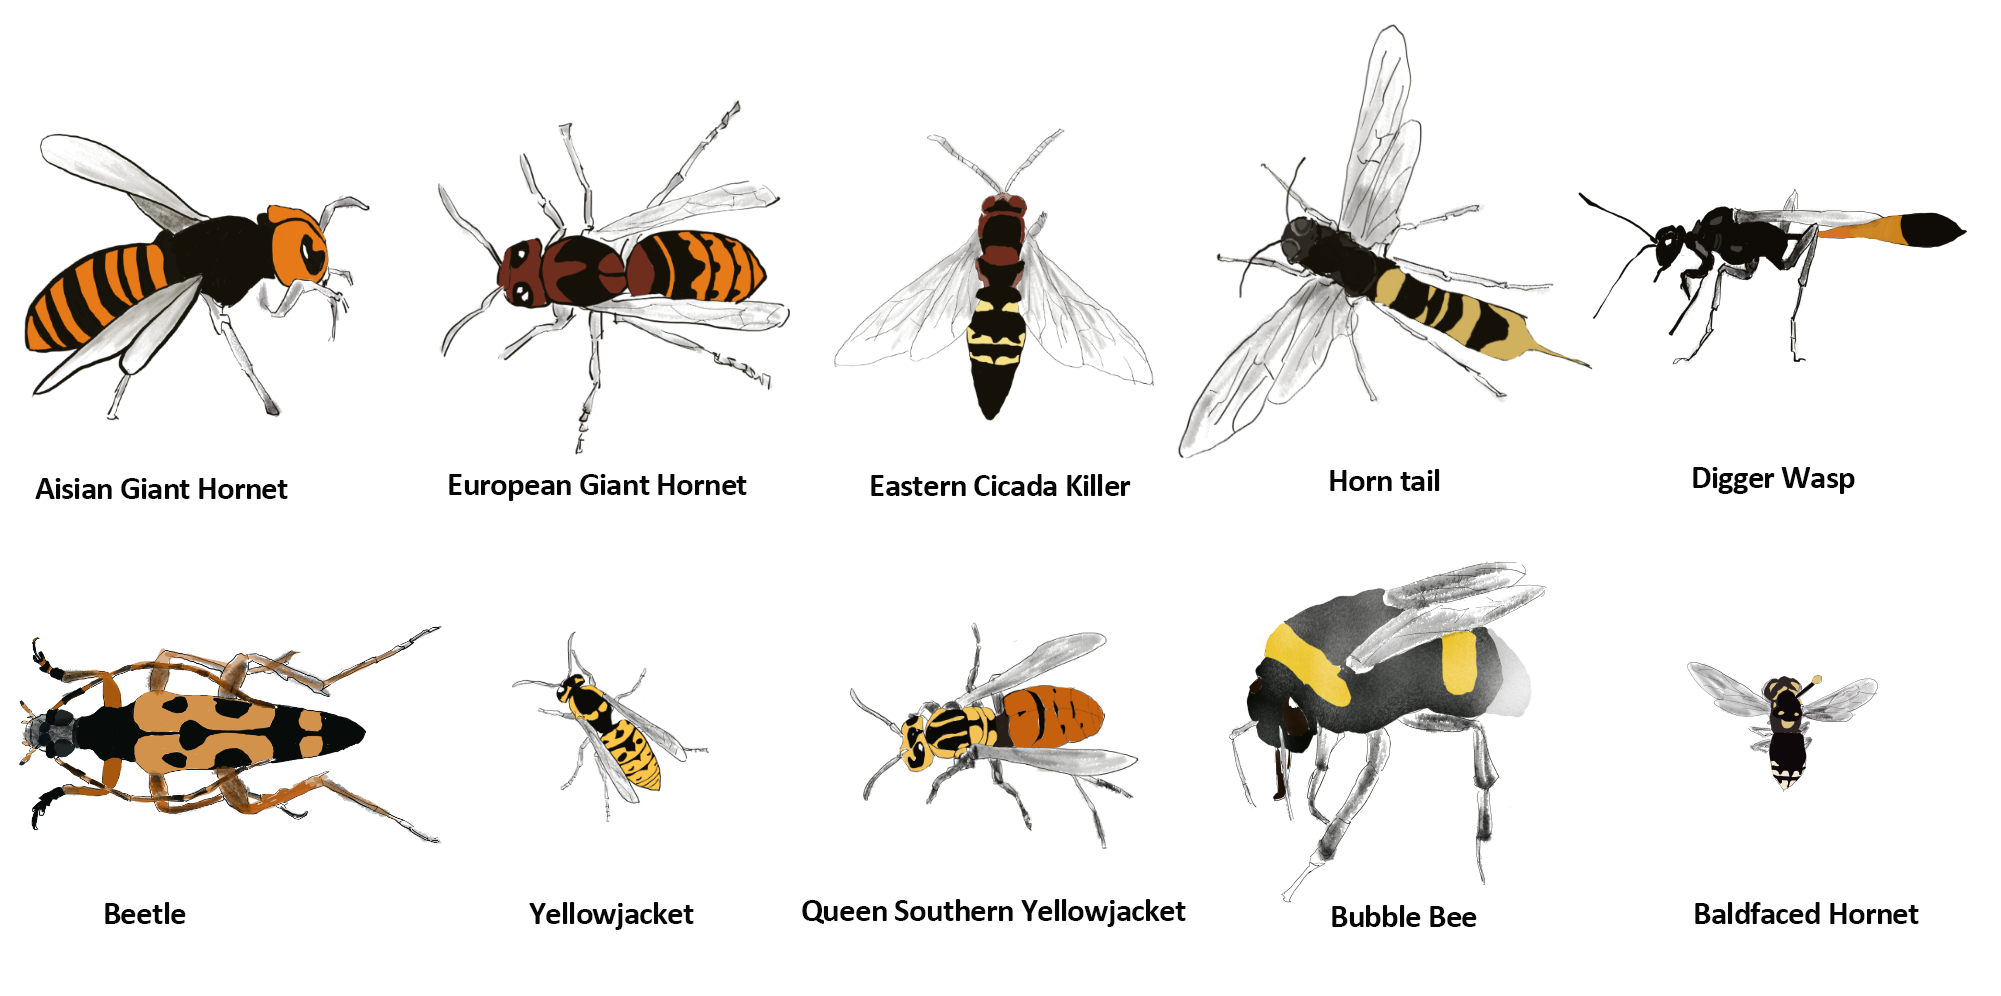
\includegraphics[scale = 0.3]{Chapter-2021C/images-2021C/2-bee.png}
    \caption{Factor features of different bees.}
    \label{fig:2021C-Factor features of different bees.}
\end{figure}


We compare the factor features of the sample with the pest's one by one. After the comparison, we value the factor $fv^i_j$ due to the similarity. The more similar the sample factor is to the pest factor, the bigger the sample's factor value is, ranging from 0 to 1. The value some samples is shown in Table \ref{tbl:2021C-FCEM factor value.}.

%%三线表 cellular automata notation
\begin{table}[H]
    \renewcommand\arraystretch{2}   %%控制行间距
    \centering
    \caption{The values of the factors.}
    \begin{tabular}{cccccc}    %%三列均左对齐
        \toprule  %%表格横线加粗
        \specialrule{0em}{2pt}{2pt}    %%添加透明线控制行高
         Type & Size (inch) & Abdomen & Head & Chest & Nest \\
        \specialrule{0em}{2pt}{2pt}    %%添加透明线控制行高
        \midrule
        \specialrule{0em}{1pt}{1pt}
        Pests & 1 & 1 & 1 & 1 & 1 \\
        European hornet & 0.9 & 0.9 & 0.6 & 0.6 & 0.6 \\
        Yellowjacket & 0.3 & 0.9 & 0.6 & 0.3 & 0.6 \\
        Queen southern yellowjacket & 0.3 & 0.6 & 0.3 & 0.6 & 0.6 \\
        Eastern cicada killer & 0.9 & 0.9 & 0.9 & 0.9 & 0.3 \\
        Baldfaced hornet & 0.3 & 0.3 & 0.9 & 0.9 & 0.3 \\
        Digger wasp & 0.6 & 0.3 & 0.9 & 0.9 & 0.3 \\
        Horn tail & 0.9 & 0.9 & 0.6 & 0.3 & 0.3 \\
        Beetle & 0.6 & 0.6 & 0.6 & 0.3 & 0.3 \\
        Bumble bee & 0.6 & 0.3 & 0.3 & 0.3 & 0.3 \\
        % Wood wasp & 0.9 & 0.9 & 0.3 & 0.9 & 0.3 \\
        \specialrule{0em}{1pt}{1pt}
        \bottomrule
    \end{tabular}
    \label{tbl:2021C-FCEM factor value.}
\end{table}

Thirdly, we apply AHP to allocate weights to factors. To begin with, we construct the judgment matrix $M$ in the order of size, abdomen, head , chest and nest.

\[
    M = \begin{pmatrix}
            1 & 1 & 3 & 4 & 6  \\
            1 & 1 & 4 & 5 & 8  \\
            \frac{1}{3} & \frac{1}{4} & 1 & 3 & 4  \\
            \frac{1}{4} & \frac{1}{5} & \frac{1}{3} & 1 & 2  \\
            \frac{1}{6} & \frac{1}{8} & \frac{1}{4} & \frac{1}{2} & 1  \\
        \end{pmatrix}
\]

After that, it is easy to solve the eigenvalues of the matrix $M$ and get the \textbf{weight vector} is $\omega = {[0.3398, 0.3986, 0.1445, 0.0732, 0.0439]}^T$.

Now we make the consistency check. Since the consistency index $CI = \frac{\lambda_{max}-n}{n-1}$ and the consistency ratio $CR = \frac{CI}{RI}$, where the random index $RI$ is only relative to the matrix size (see in Table \ref{tbl:2021C-The value of RI}). By calculating, we get $CR = 0.0261<0.1$, which passes the consistency check.

%%The value of RI
\begin{table}[H]
    \renewcommand\arraystretch{2}   %%控制行间距
    \centering
    \caption{The value of $RI$.}
    \begin{tabular}{ccccccccc}    %%三列均左对齐
        \toprule  %%表格横线加粗
        \specialrule{0em}{2pt}{2pt}    %%添加透明线控制行高
        matrix size & 2 & 3 & 4 & 5 & 6 & 7 & 8 & 9 \\
        \specialrule{0em}{2pt}{2pt}    %%添加透明线控制行高
        \hline
        \specialrule{0em}{1pt}{1pt}    %%添加透明线控制行高
        $RI$        & 0 & 0.58 & 0.90 & 1.12 & 1.24 & 1.32 & 1.41 & 1.45  \\
        \specialrule{0em}{1pt}{1pt}    %%添加透明线控制行高
        \bottomrule
    \end{tabular}
    \label{tbl:2021C-The value of RI}
\end{table}

To conclude, we can get the following $v_i$ formula as 
\begin{equation*}
    v_i = 0.3398 \times fv^i_1 + 0.3986 \times fv^i_2 + 0.1445 \times fv^i_3 + 0.0732 \times fv^i_4 + 0.0439 \times fv^i_5
\end{equation*}

\subsection{Discuss FCEM-AHP Consequence }
From the above formula, we can calculate and obtain the value of each type of bees in descending order in Figure \ref{fig:2021C-The FCEM Consequence.}.

\begin{figure}[H]
    \centering
    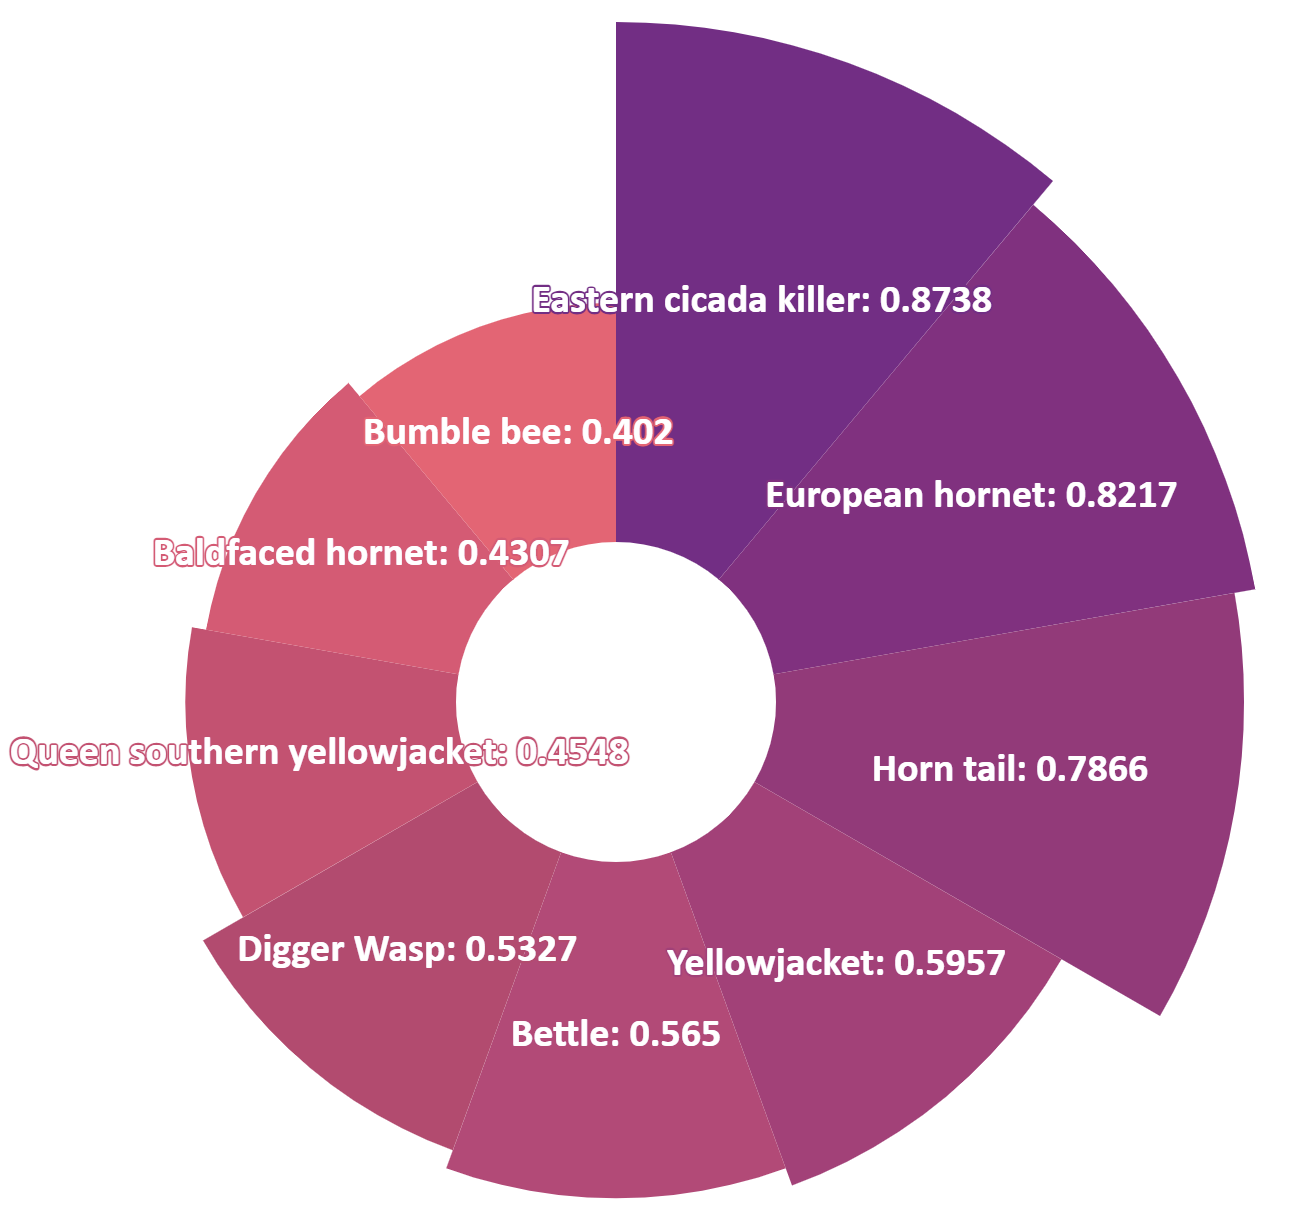
\includegraphics[scale = 0.25]{Chapter-2021C/images-2021C/2-result.png}
    \caption{Similarity to the pest.}
    \label{fig:2021C-The FCEM Consequence.}
\end{figure}



%%三线表 FCEM consequence
% \begin{table}[H]
%     \renewcommand\arraystretch{2}   %%控制行间距
%     \centering
%     \caption{The $FCEM$ Consequence.}
%     \begin{tabular}{cc}    %%三列均左对齐
%         \toprule  %%表格横线加粗
%         \specialrule{0em}{2pt}{2pt}    %%添加透明线控制行高
%          Type & Value \\
%         \specialrule{0em}{2pt}{2pt}    %%添加透明线控制行高
%         \midrule
%         \specialrule{0em}{1pt}{1pt}
%         Pest & 1.0000 \\
%         Eastern cicada killer & 0.8738 \\
%         % Wood wasp & 0.8738 \\
%         European hornet & 0.8217 \\
%         Horn tail & 0.7866 \\
%         Yellowjacket & 0.5957 \\
%         Beetle & 0.5650 \\
%         Digger wasp & 0.5327 \\
%         Queen southern yellowjacket & 0.4548 \\
%         Baldfaced hornet & 0.4307 \\
%         Bumble bee & 0.4020 \\
%         \specialrule{0em}{1pt}{1pt}
%         \bottomrule
%     \end{tabular}
%     \label{tbl:2021C-FCEM consequence.}
% \end{table}

The consequence implies that the most three similar types of insects to the pest is \textbf{Eastern cicada killer}, \textbf{European hornet}, and \textbf{Horn tail}. Therefore, the likelihood of mistaken classification of them also rank the top three. 

\vspace{1cm}

\section{Report Prioritization}
Before our study, we first preprocess the data set. We delete the data with illogical detection date, such as one data with detection date $4/21/1600$. Additionally, we erase the data whose submission day is earlier than its detection day which is apparently irrational. After the above operations, we get the processed 4411 pieces of data set.
\subsection{General Idea}
When evaluating a sighting report, the first thing that needs to be judged is its amount of information. If its information is lacking then it is very likely to be classified as unverified. Such a report is not worthy of more analysis. Secondly, it needs to be prioritized by judging the possibility of its occurrence based on its existing information including latitude and longitude, detection date, and notes.

Next, according to the latitude and longitude, we can obtain the \textbf{possibility of pests appearing in the area} based on PS-CA model. Besides, we can judge the \textbf{likelihood of pests appearing at this time} from the detection time and pest habits. \textbf{The certainty expressed in the description} extracted from the note is also an important factor. From the image information, \textbf{the similarity between the observed insect and the pest} can be calculated by FCEM-AHP model. 

Then we use a multi-index evaluation method considering these four factors to prioritize the sighting reports. Our model idea is shown in Figure \ref{fig:idea}.
\begin{figure}[H]
    \centering
    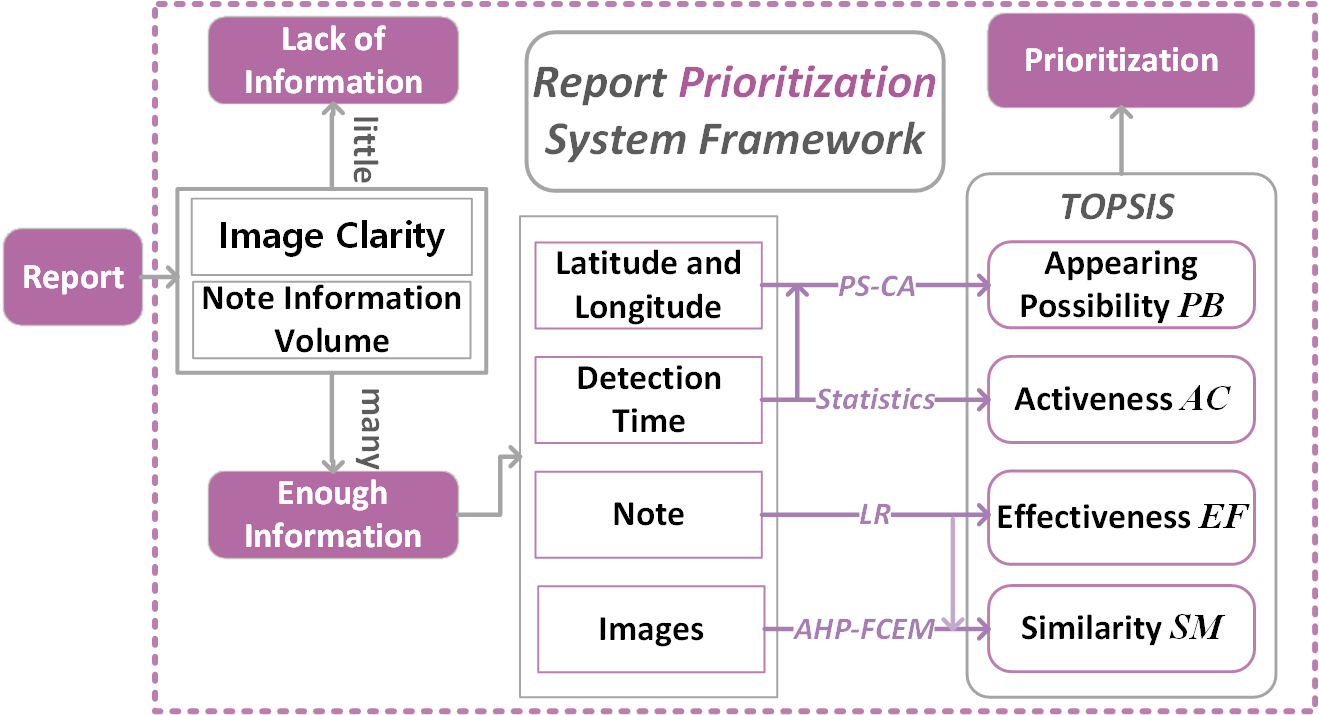
\includegraphics[scale = 0.5]{Chapter-2021C/images-2021C/3-idea.png}
    \caption{Report Prioritization System Framework}
    \label{fig:idea}
\end{figure}

\subsection{Data Screening}

In the sighting report, the most important part is the image. Therefore, image recognition will play an important role in prioritizing reports. In fact, due to the scarcity of correct samples, we cannot train a powerful machine learning system in a limited time. So we changed our thinking and rely on the existing robust insect recognition platform to perform image recognition.

First, we associate the GlobalID of each report with the image file name.

Then we upload the image to a website\cite{insect} with an accuracy of about 78.45\%, which can recognize the image and output the name of the insect in the image. Of course, if the image is blurry or there are no insects in it, it will output ‘no insects’ results.

If the website can not identify the insect in the picture, we assume that the information of this picture is not enough for the judgement and will be placed in a screen-out zone. 

For those reports in the screen-out zone, we calculate the informative score of the given notes by logistic regression to determine whether this certain report will be screened out or not.

To calculate the informative score of the given notes, we need to assign every word appearing in the report with a score to depict its amount of information. As logistic regression is a widely-used algorithm for binary classification, we use logistic regression to judge whether a certain word is informative or not:
\vspace{0.5cm}

\begin{algorithm}[H]
\caption{Logistic Regression}
  \KwIn{Notes set $\mathcal{N}=\{ n_1, n_2, \dots, n_k \}$, Labels set $\mathcal{L}=\{ l_1, l_2, \dots, l_k \}$}  
  \KwOut{Words informative scores $\mathcal{S}$}  
  Construct an ideal score set of all the notes
  
  $\mathcal{SN}_{ideal}=\{ sn_1, sn_2, \dots, sn_k \}$:
  
  \For{$n_i$ \text{in notes set} $\mathcal{N}$}{
   \If{\text{the label} $l_i$ of $n_i$ \text{is Positive or Negative}}{ 
        $sn_i=1$, which means that this note has enough information
    }
    \ElseIf{$l_i$ \text{is Unverified}}{
        $sn_i=0$, which means that this note is lack of information
    }
  }
  Train the words informative scores to minimize the loss function:
  $\mathcal{S}=argmin(\sum_{i=1}^k (sn_i-\frac{1}{1+e^{\sum s\in\mathcal{S}}})^2)$
  
\end{algorithm}

Trained words informative scores are shown in the following word cloud:
\begin{figure}[H]
    \centering
    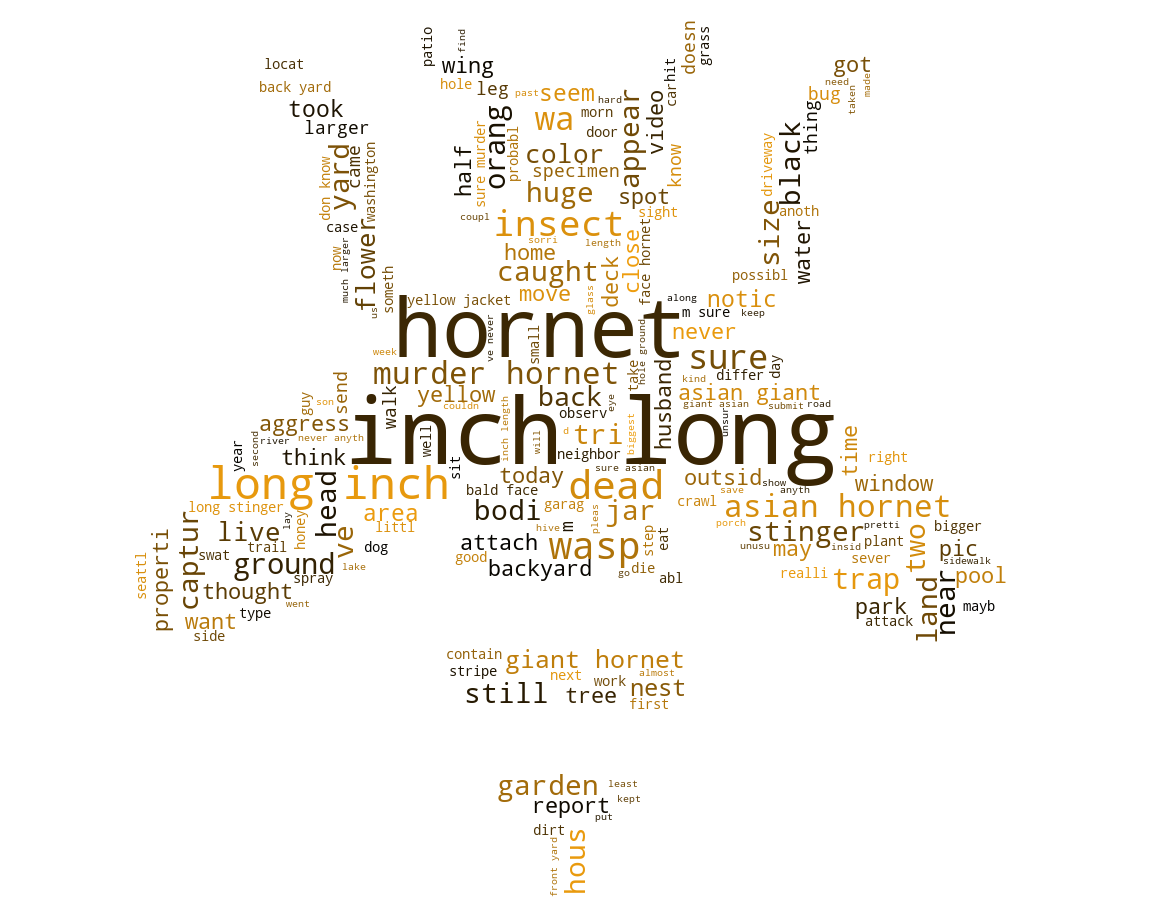
\includegraphics[scale = 0.3]{Chapter-2021C/images-2021C/3-word cloud.png}
    \caption{Word cloud of informative score}
    \label{fig:word cloud}
\end{figure}


Then we use the sigmoid funtion to define the informative score of the whole note. For the note of a new report $rp$, its informative score $S_{rp}$ is defined as:

\begin{equation*}
    S_{rp} = \frac{1}{1+e^{\sum_{i=0}^k s_i}}
\end{equation*}

where $s_i$ represents the informative score of the $i^{th}$ word in this report notes. 

For a report $rp$ in the screen-out zone, (which means that its picture can not be identified by the insect classification website), $rp$ will be screened out in this term if $S_{rp}<0.5$.


\subsection{Report Prioritization based on TOPSIS}
In this section, we use \textbf{Technique for Order Preference by Similarity to an Ideal Solution (TOPSIS)} to prioritize the reports most likely to be positive sightings.

The TOPSIS method \parencite{TOPSIS} is a multiple attribute decision-making method. For example, Zhongyou Xing has studied the introduction of foreign players in CBA games on the application of TOPSIS \parencite{TOPSIS-CBA}.

The TOPSIS method choose several evaluation indices towards the samples, normalize the indices, obtain the best and the worst vector value, calculate the distance between the sample and the best and worst vector, and calculate the relative approach degree.

Finally, the sample is ordered by the value of the relative approach degree.

Continuing the analysis in section 4.1, we define the four influencing factors in details and design strategies to obtain them. These four indices notations is shown in Table \ref{tbl:2021C-Notations of TOPSIS indices.}.

%%三线表 cellular automata notation
\begin{table}[H]
    \renewcommand\arraystretch{2}   %%控制行间距
    \centering
    \caption{Notations of TOPSIS indices.}
    \begin{tabular}{ccc}    %%三列均左对齐
        \toprule  %%表格横线加粗
        \specialrule{0em}{2pt}{2pt}    %%添加透明线控制行高
        Symbol & Definition & Notes \\
        \specialrule{0em}{2pt}{2pt}    %%添加透明线控制行高
        \midrule
        \specialrule{0em}{1pt}{1pt}
        $RP$ & the set of reports & $RP = \{ rp_1, rp_2, \dots, rp_n \}$ \\
        $PB$ & the set of possibility of pest emerging & $PB = \{ pb_1, pb_2, \dots, pb_n \}$ \\
        $AC$ & the set of activeness of pests & $AC = \{ ac_1, ac_2, \dots, ac_n \}$ \\
        $EF$ & the set of note effectiveness of reports & $EF = \{ ef_1, ef_2, \dots, ef_n \}$ \\
        $SM$ & the set of similarity of the reports to pests & $SM = \{sm_1, sm_2, \dots, sm_n \}$ \\
        \specialrule{0em}{1pt}{1pt}
        \bottomrule
    \end{tabular}
    \label{tbl:2021C-Notations of TOPSIS indices.}
\end{table}

In all, a sample report $rp_i$ contains four indices, which can be represented by 
\begin{equation*}
    rp_i = \{ pb_i, ac_i, ef_i, sm_i \}.
\end{equation*}

\begin{enumerate}[\quad\bf 1.]
\item \textbf{Emerging Possibility of the Pest by PS-CA model}%由经纬度获得概率密度

As a result of the \textbf{PS-CA model}, we have the state of every cell $s_{i,t}$ in the cellular automata after the entire simulation. Regarding the meaning of cell state, $s_{i,t}$ represents the degree of the bee gathering of the $i^{th}$ cell at time $t$. 

\begin{figure}[H]
    \centering
    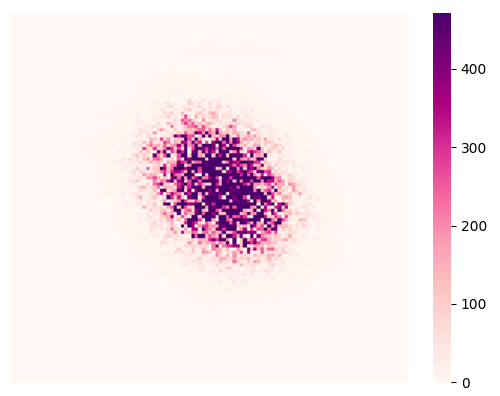
\includegraphics[scale = 0.5]{Chapter-2021C/images-2021C/4-relitu.png}
    \caption{Emerging Possibility of the Pest after one year simulation.}
    \label{fig:2021C-relitu}
\end{figure}

In terms of a sample report $rp_i$, we transfer its detection time to the simulation time $t$. Next, we calculate the cell number $j$ with the longitude and latitude of the report. Consequently, we get the state $s_{j,t}$. Finally, we divide it by the maximum state of all cells to obtain the index $pb_i = \frac{s_{j,t}}{\max \{ s_{k,t} \}}, k=(1, 2, \dots, n)$. Figure \ref{fig:2021C-relitu} shows our results for one year simulation.

\item \textbf{Activeness of the Pest by time}%定义各月份活跃度
%%可以补reference

From the introduction of the pest, we know that pests are only seen outside the nest from spring to hibernation\parencite{NPRG}. It can imply that pests' activeness differs on the basis of time. We define the activeness to be 1 from May to December, and 0.5 otherwise.

Regarding a sample report $rp_i$, we get the $month$ from its detection time and have the activeness $ac_i$ through

\begin{equation*}
    ac_i = \begin{cases}
    1 &, \text{month}=5, 6, 7, 8, 9, 10, 11, 12; \\
    0.5 &, \text{otherwise}.
    \end{cases}
\end{equation*}

\item \textbf{Note Effectiveness}

Similar to what we have done in Section 4.2 Data Screening, we train the informative score of all the words appearing in the reports and calculate a total informative score of every piece of note using the sigmoid function. For the note of a new report $rp$, its informative score $S_{rp}$ is defined as:
\begin{equation*}
    ef_{rp} = S_{rp} = \frac{1}{1+e^{\sum_{i=0}^k s_i}}
\end{equation*}

where $s_i$ represents the informative score of the $i^{th}$ word in this report notes. 

However, there is some difference between this part and the informative scores training in Section 4.2. In Section 4.2, labels of the trained notes are 'Have enough information' and 'Lack of information', while in this part, labels are 'Positive' and 'Negative'. The former aims to tell the difference between informative notes and those that are not, while the latter distinguish the Positive ID from the Negative.


\item \textbf{Possibility of misclassification of image recognition}

With the help of the insect recognition website\cite{insect}, we can get the general class of the insect in the pictures by using a simple script to upload them and read the results on the website. Then, we can obtain the similarity between the insect and the pest based on the recognition result and the FCEM-AHP model. The reason for using similarity as an evaluation index instead of directly relying on insect recognition websites is that recognition has uncontrollable errors, and we can reduce errors as much as possible by combining the results with similarity as an index.
 
For example, we randomly select a report with a GlobalID of {2CE88ACB-6B4B-4357-91F1-813D079B5057}, and the attached image name is ATT154\_20200512\_180734. The result of the image being identified on the website is a yellow jacket. The similarity between yellowjacket and the pests studied by us is 59.57\%, so its $sm$ value is 0.5957.

%Based on the AHP-FCEM model in section 3, we can finally get a value $v_i$, which we denotes as the similarity. As for a sample report $rp_i$, we follow the rules of the AHP-FCEM model to get the value. By artificially examining the picture and note of the report, we fill in the value of five factors $FV^i$ according to the definition of the AHP-FCEM model and calculate the value $v_i$. Then we simply get the similarity $sm_i$ by $sm_i = v_i$.

\end{enumerate}

After obtaining all the values of the indices, we run the TOPSIS method to prioritize the top-ranked reports, which we regard as most likely to be positive sightings.

But theoretical reasoning is not enough. We randomly selected two positive reports, two negetive reports, two unverified reports and 14 unprocessed reports from the report set for testing. Their numbers are 1, 2, \dots , 20. Their processing and calculation procedures are shown in Figure \ref{fig:result of the prioritization system}.
\begin{figure}[H]
    \centering
    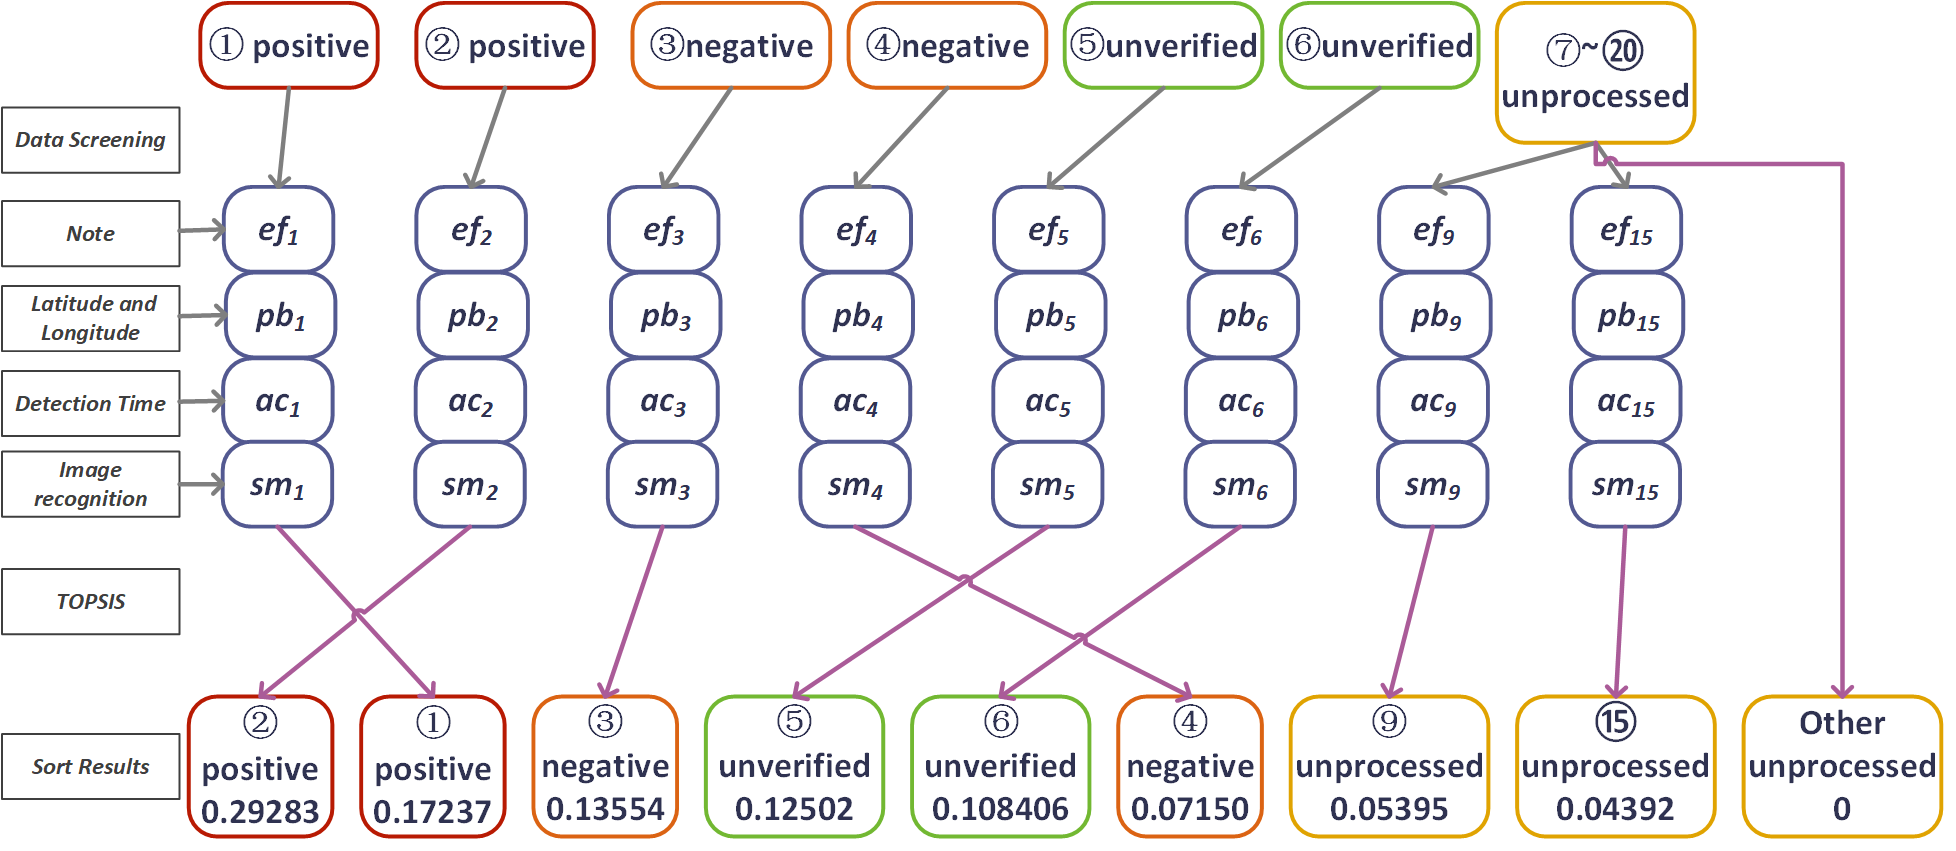
\includegraphics[scale = 0.4]{Chapter-2021C/images-2021C/3-result.png}
    \caption{The test result of the prioritization system (the priority decreases from left to right).}
    \label{fig:result of the prioritization system}
\end{figure}

This test result is in line with expectations and reality. Both positive reports are ranked at the forefront, which shows that our prioritization system is effective.

\vspace{1cm}

\section{Model optimization and sensitivity analysis}
\subsection{Add new starting point or delete existing point.}
DNA evidence \parencite{pestfr} showed that the hornets in Washington and Vancouver were unrelated and came from different nests \parencite{attachment}, which suggests that there is more than one pest invasion time and place. Therefore, for our spread model, it may have multiple starting points. In addition, the government's vigorous crackdown method is to directly destroy the Hornet's nest, which will have a greater impact on our simulation results. Therefore, after every nest destruction, our simulation model also needs to be adjusted accordingly.

When new reports are given over time, we may encounter a problem that some verified hornet locations is outside of our simulated area. Regarding how to determine that this new pest emergence point is a new invasion point, we have the following update mechanism.
\begin{itemize}
    \item In these extracted reports, we find the most earliest one due to its detection time.
    \item Then we add a new starting point at this place on its detection date and set the initial population as 200.
    \item We run the PS-CA model again from the first day and we repeat the above steps until all the given positive reports are included in our simulation region.
\end{itemize}

By contrast, the government has taken actions to interfere with the pest spread. When an existing nest is destroyed, we clear the state number of the place in our cellular automata model immediately.

%%插图 标点精确度分析
\begin{figure}[H] 
\begin{minipage}[t]{0.5\linewidth} 
\centering 
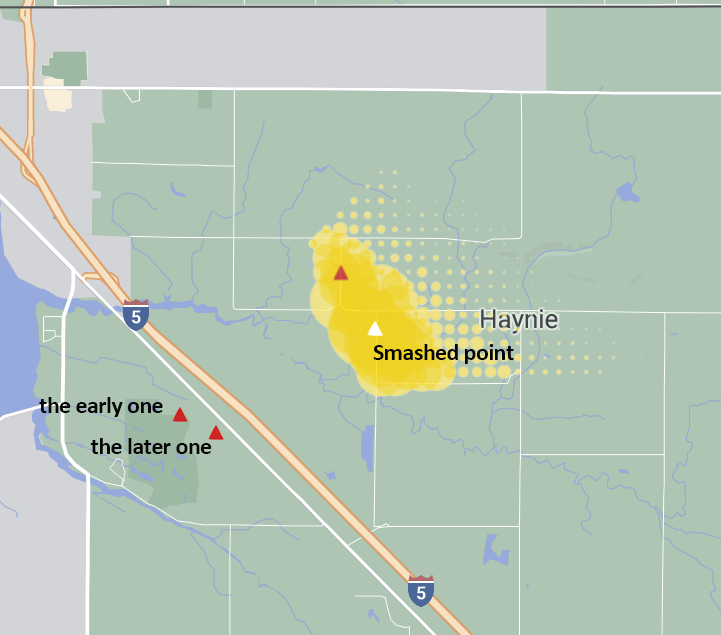
\includegraphics[width=2.5in]{Chapter-2021C/images-2021C/4-before.png} 
\caption{Before update.} 
\label{fig:2021C-4Before update.} 
\end{minipage}
\begin{minipage}[t]{0.5\linewidth} 
\centering 
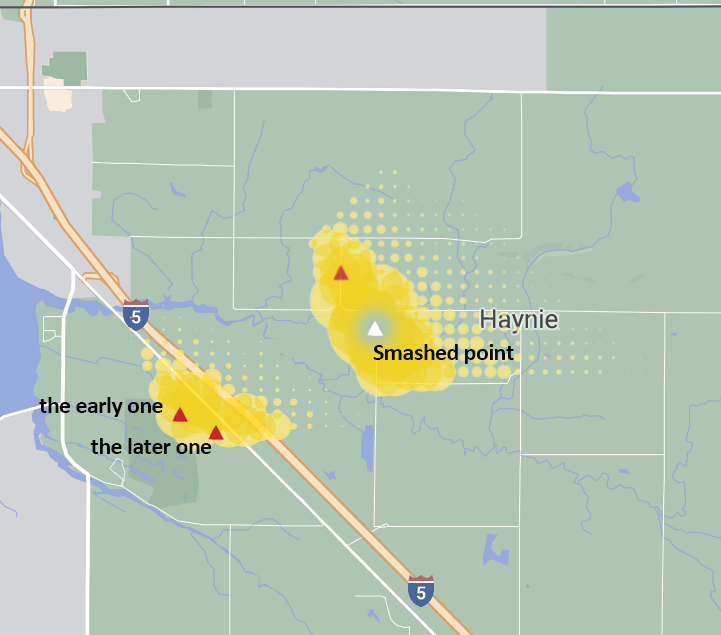
\includegraphics[width=2.5in]{Chapter-2021C/images-2021C/4-after.png} 
\caption{After update.} 
\label{fig:2021C-4After update.} 
\end{minipage} 
\end{figure}

The former Figure \ref{fig:2021C-4Before update.} and \ref{fig:2021C-4After update.} is an example of our update rule. The picture on the right vividly shows how we add a new starting point and delete an existing point.

Due to the uncertainty of the time of pest invasion and destruction, we must update the simulation mechanism every time we receive a nest change.

\subsection{Adjust Pest Growth Curve}
Initially, we ignore the impact of human intervention and environmental capacity on the growth and reproduction of pest, so we set its growth curve as a J-type growth. And now, due to the government's destruction of pest nests, we should consider this impact.

It is known from the literature that the annual population loss of bees is about 9.5-10.7\% \parencite{Chinesebee}. This is almost the same for Vespa mandarinia  in the same suborder as bees. As for human intervention factors, we can't get a precise impact number, so we might as well assume that the population of pests is decreasing year by year, that is change $\lambda$ from 1.2 to 0.8. 
As for the update frequency, we recommend that it be adjusted once a year based on the government's prevention and control efforts.

\subsection{Eradication Evidence Constitution and Sensitivity analysis}

To investigate whether or not the pest has been eradicated in Washington State, we define an index $Degree_{eradication}$ for the degree of eradication. The index is calculated by the quotient of the total number at $t$ time and the initial number. We set three limits to the index as to show the degree of eradication. More thorough eradication implies smaller index.

\begin{equation*}
    \label{eq:degree}
    Degree_{eradication} = \frac{\sum^n_{i=1} p_{i,t}}{p_{start,1}} \begin{cases}
    <1, & \text{under control but still need more intervention}; \\
    <0.1, & \text{effective but still need more observation}; \\
    <0.01, & \text{thorough eradication}.
    \end{cases}
\end{equation*}

Based on the degree of eradication, we run the cellular automata model to calculate the intervention period until the degree satisfy the criteria. In addition, we make sensitivity analysis towards the intervention period related to $\lambda$.

%%插图 sensitivity analysis
\begin{figure}[H] 
\begin{minipage}[t]{0.5\linewidth} 
\centering 
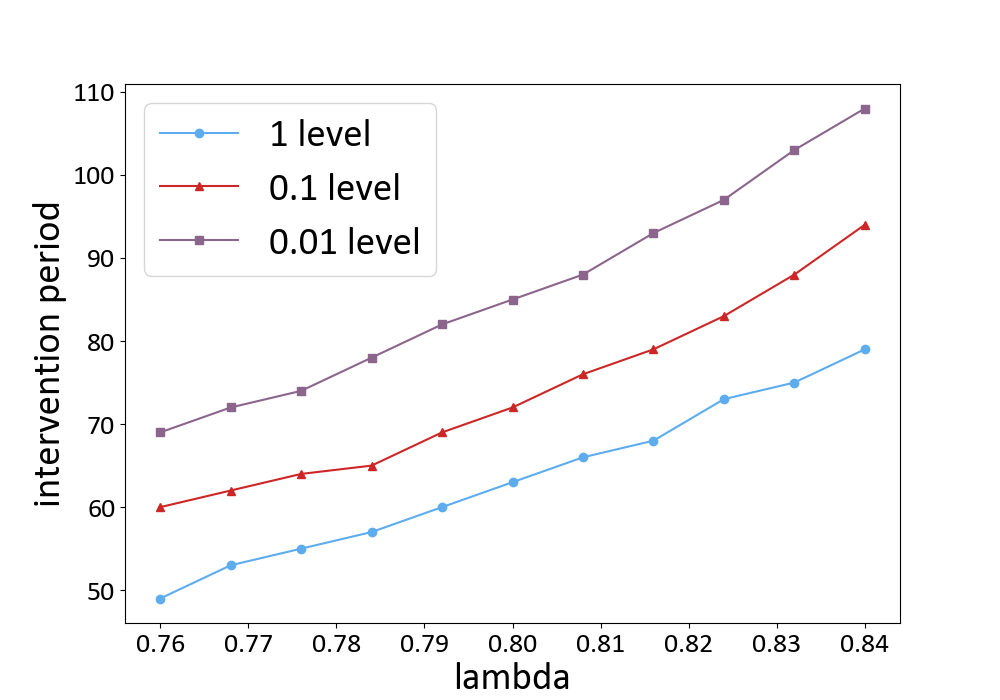
\includegraphics[width=3in]{Chapter-2021C/images-2021C/4-sensitivity.png} 
\caption{Intervention period.} 
\label{fig:2021C-Intervention period.} 
\end{minipage}
\begin{minipage}[t]{0.5\linewidth} 
\centering 
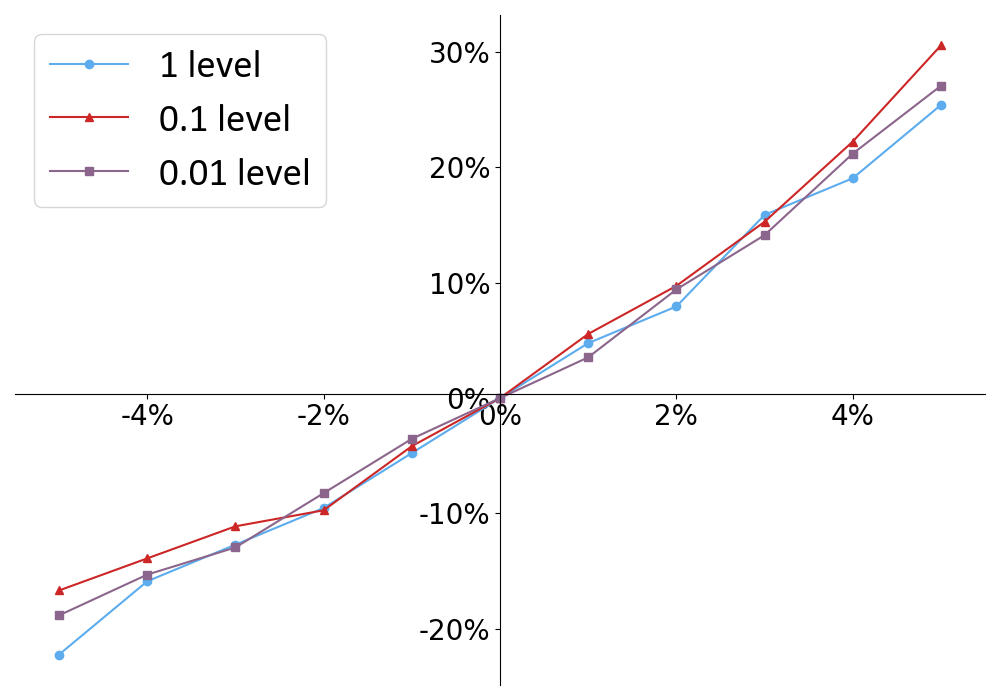
\includegraphics[width=3in]{Chapter-2021C/images-2021C/4-degree.png} 
\caption{Sensitivity analysis.} 
\label{fig:2021C-Sensitivity analysis.} 
\end{minipage} 
\end{figure}

Figure \ref{fig:2021C-Intervention period.} shows that high level of eradication needs longer period of intervention. Meanwhile, the sensitivities of the intervention to the value of $\lambda$ are similar regarding different eradication level in Figure \ref{fig:2021C-Sensitivity analysis.}.

In conclusion, our model is stable in different eradication levels and more efforts are needed to achieve a more exhausive level of eradication.

\vspace{1cm}

\section{Conclusions}
In the summary session, we proudly believe that we have solved a big problem for the Washington State Department of Agriculture. 

First of all, we use the cellular automata model to simulate the geographical distribution of the pests, and conclude that if the pest are not prevented and controlled in time, the consequences will be raging. At the same time, the accuracy of our simulation model can reach an area of $150m \times 150m$.

Secondly, we combine FCEM and AHP to calculate the possibility of other types of insects being misclassified as pests. The results show that the eastern cicada killer, European hornet and horn tail are the three most likely insect to be misclassified visually.

Thirdly, we use LR to filter the reports, and the filtered reports get a comprehensive score based on TOPSIS from the four dimensions. And finally we get the priority ranking of the sighting reports. In order to fully test the accuracy of this system, we randomly selected samples to test and get the desired results.

Fourthly, we establish a model update mechanism from two aspects: new pest invasion points and human intervention prevention and control. And we determine the update frequency based on existing data to be updated once every new intrusion point appears and once a year. 

Finally, we use the current number of existing pests in each cell as a measure and set three indicators for eradicating pests. And we test the sensitivity of the optimized model to prove that our model is stable.

\vspace{1cm}

\section{Strengths and Weaknesses}
\begin{large}
\textbf{Strengths:}
\end{large}

\begin{itemize}
    \item \textbf {Data processing and sreening.} Although it is difficult to analyze text and images, we still succeed in effectively filtering reports based on text and images.
    \item \textbf {Divergent thinking.} A powerful machine learning system relies on a large number of correct samples, which we believe is not suitable for this problem. So we divergently rely on the help of the existing image recognition system, and minimize its errors from multiple dimensions.
    \item \textbf {Visualization.} We vividly and diversely display various results and ideas for thinking about problems. And, we use visualization to show the source of some data extraction, such as in the AHP model.
    \item \textbf {Robust model.} Our PS-CA model achieves a high degree of fit simulation result with only a small number of correct samples.
    \item \textbf {Solve from a multidisciplinary perspective.} Based on the problem background, we use the knowledge of population growth in biology to formulate rules for the model.
\end{itemize}

\begin{large}
\textbf{Weaknesses:}
\end{large}

\begin{itemize}
    \item In our model, the calculation of some synthesized variables is subjective, lacks credibility, and requires a lot of data to verify.
    \item Our model does not consider that pests will spread over longer distances due to human activities\parencite{simulation}.
    \item Our spread model only considers the vegetation in the area when determining the environmental factors that affect the spread of pest. If there is sufficient time and advanced technology, we can also perform niche modeling based on climate and precipitation.
    \item It is a pity that we are unable to rank all 4441 reports due to time constraints, so we finally failed to get a statistically correct rate.
\end{itemize}

\newpage
\section{Memorandum}
\noindent\textbf{Date:} February 9, 2021\\
\textbf{To:} the Washington State Department of Agriculture\\
\textbf{From:} MCM Team 2100585\\
\textbf{Subject:} Identifying the sighting reports of Vespa mandarinia\\
\rule[-7pt]{14.3cm}{0.1em}

\noindent Dear Sir or Madame,

In accordance to your requests, we establish a system for prioritizing sighting reports and we also analyze relevant information about pest through data analysis. 
    Then we are writing to report our key results in these four days.

\centerline{\bf Prioritization System}
We will introduce the priority ranking system we designed from the order of the data processing flow.
\begin{enumerate}[\quad\bf Step1.]
    \item \textbf{Image Recognition.} We use the ready-made insect recognition platform with high accuracy to recognize the pictures in the report, and the output result is the name of a certain insect or it cannot be recognized. If the result is the latter then it will be put in screen-out zone. If it is the former then save the insect name.
    \item \textbf{Text processing.} We use logistic regression to measure the validity of the text in the report, and finally output a score. 
    \item \textbf{Data Screening.} If the score of a report in the screen-zone is lower than the threshold we set, the report will be discarded.
    \item \textbf{Run PS-CA model.} Based on the CA model, we simulate the regional distribution of pests over time. And then get the probability of pests appearing in the area under the detection time.
    \item \textbf{Get scores for four indices.} The first indicator is the probability of pest appearing here ,which has been obtained in Step4. The second one is the activeness of the pest at this time, which can be obtained by the pest’s habits. The third one is the information of note, which has been obtained by Step2. The fourth one is the similarity between the insects identified by the image and the pest, which can be obtained in the FCEM-AHP model according to the names of the insects.
    \item \textbf{Sorting based on TOPSIS.} In the last step, we only need to use TOPSIS to rank each report according to the scores of the four indicators.
\end{enumerate}

\centerline{\bf Conclusions}

In order to better present our conclusions, we visualize all the results and present them below.

\begin{figure}[H]
    \centering
    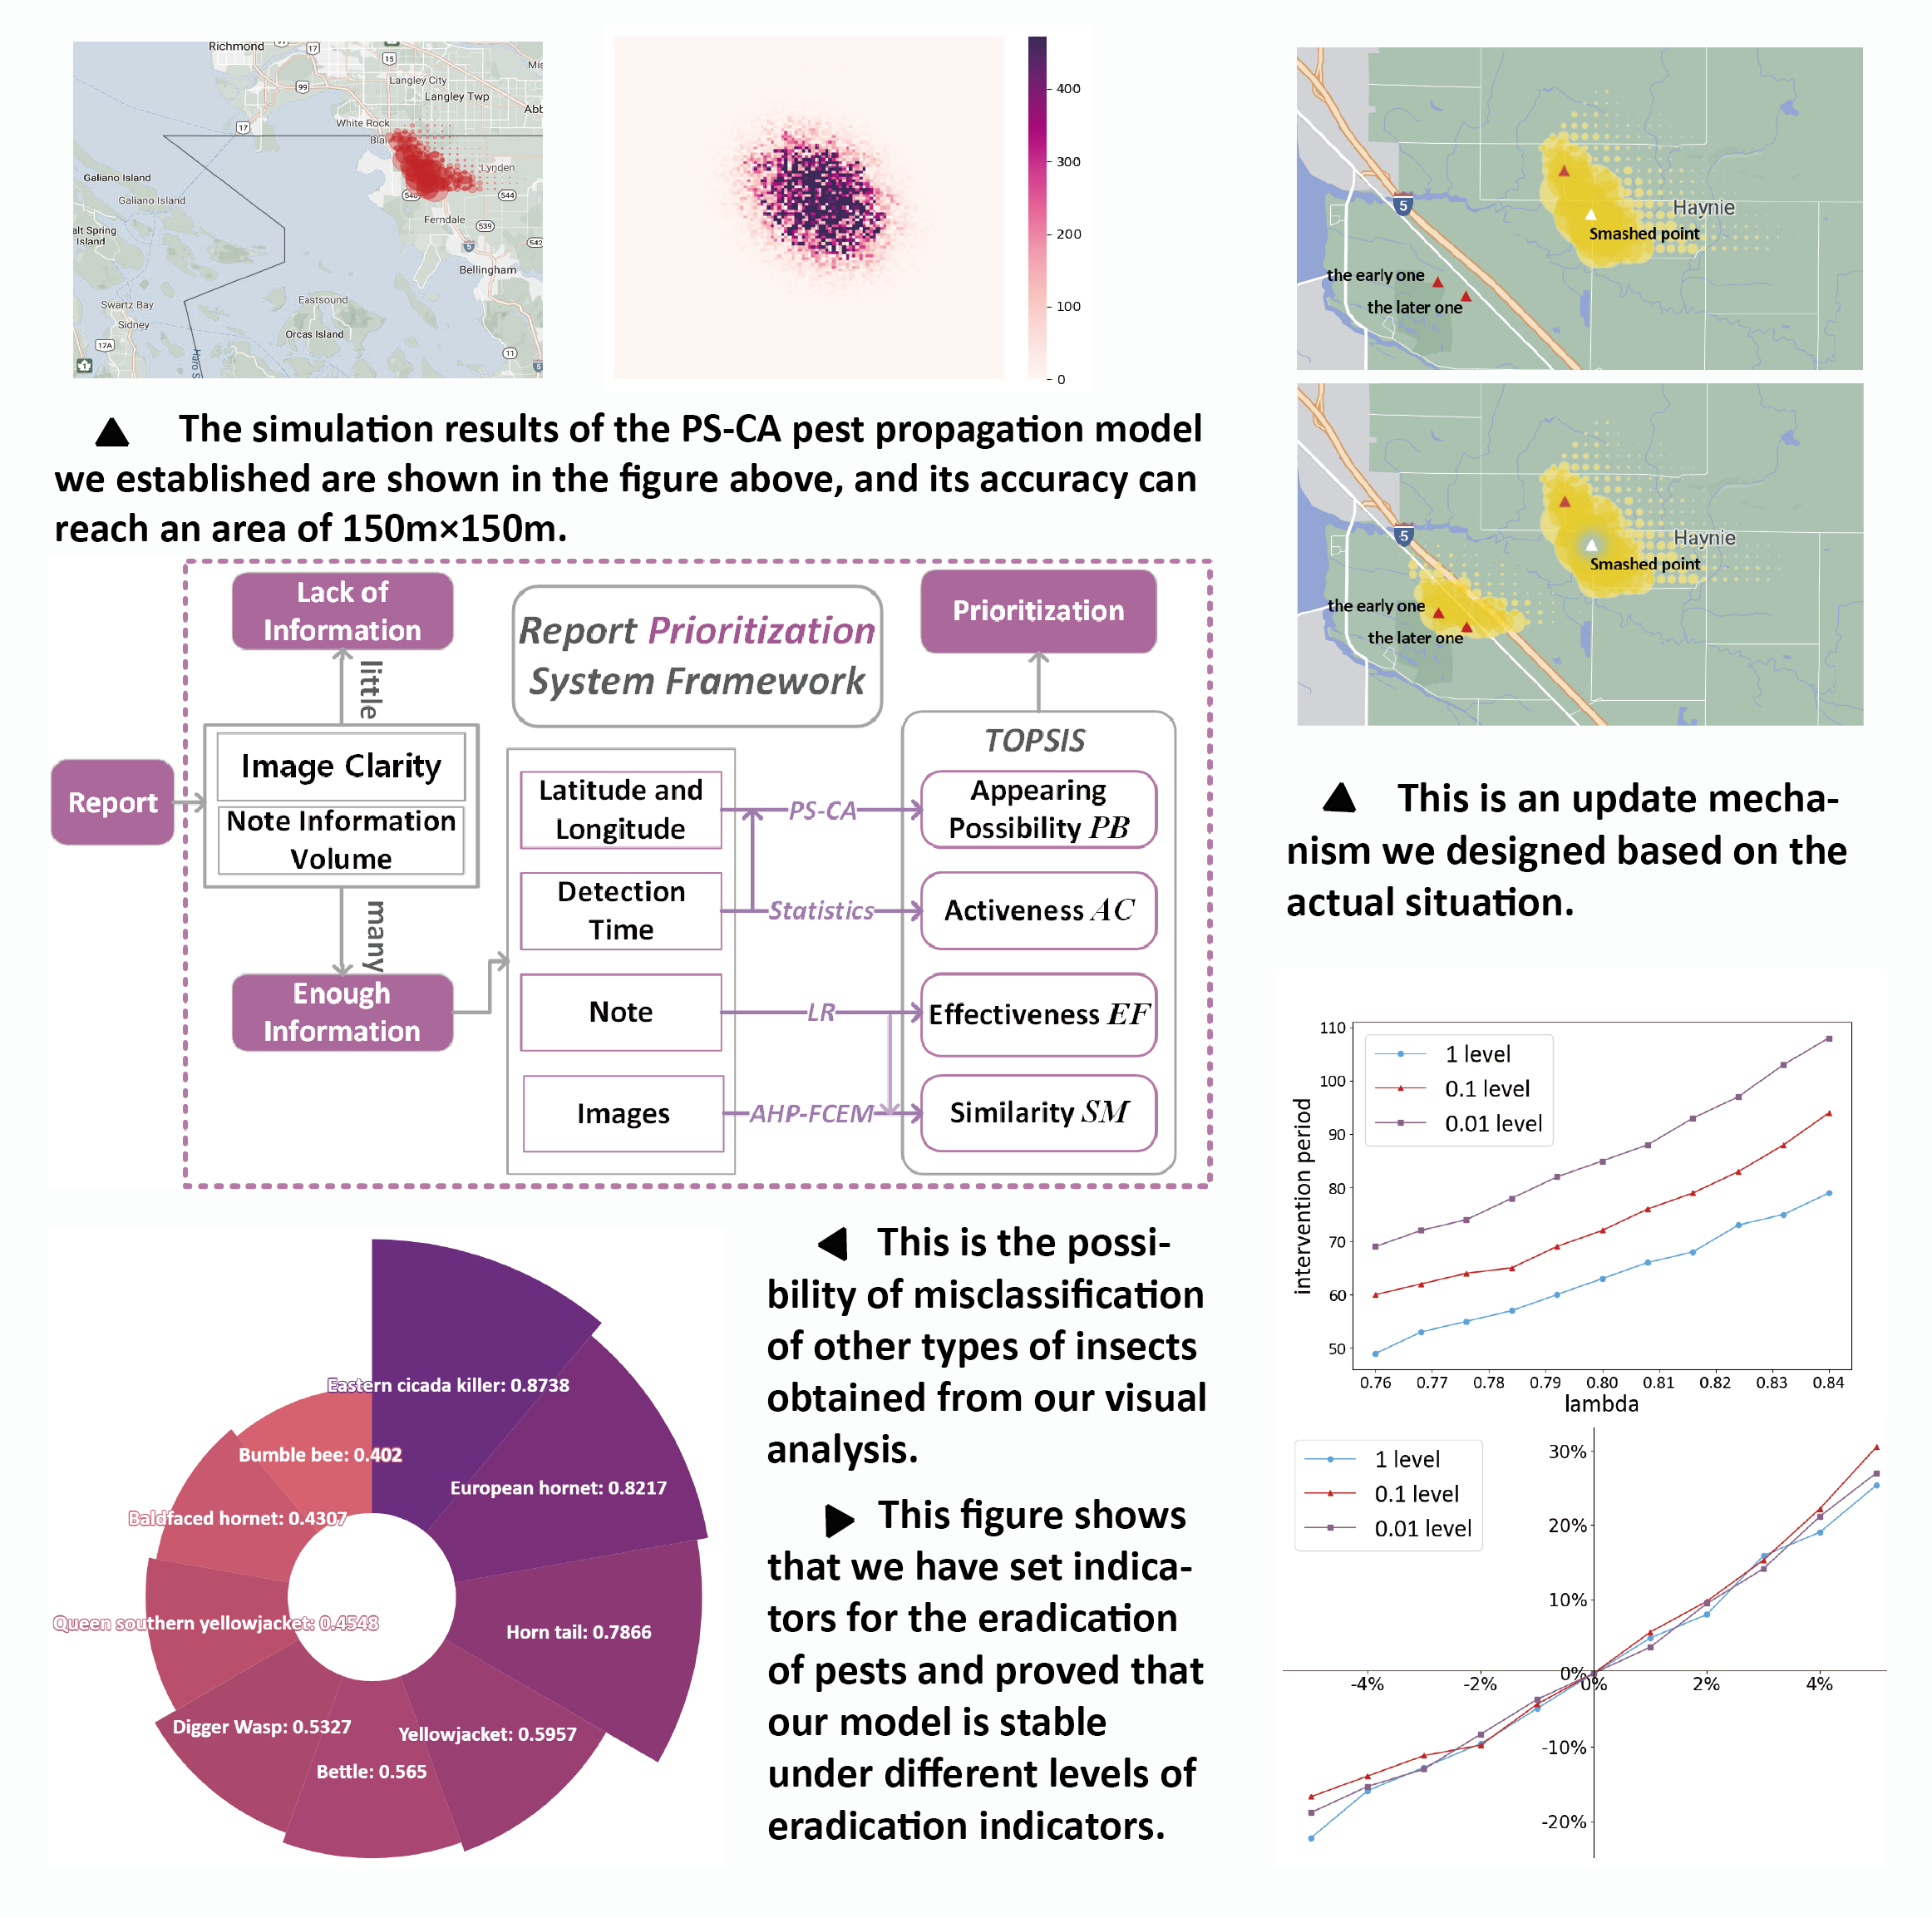
\includegraphics[scale = 0.7]{Chapter-2021C/images-2021C/post.png}
    % \caption{Emerging Possibility of the Pest after one year simulation.}
    % \label{fig:2021C-relitu}
\end{figure}
\vspace{-0.5cm}
\begin{enumerate}[\quad\bf1.]
    \item Our team established a model called \textbf{PS-CA }. This simulation is based on Washington's vegetation coverage and cellular automata model. The simulation results are shown in this paper. Moreover, its accuracy can achieve the precision of a $150m \times 150m$ area.%记得写预测结果和精度
    \item The \textbf{FCEM-AHP model} is applied to evaluate likelihood of mistaken classification from a visual perspective. In this article, we present the result of the similarity of nine types of insects of pest. 
    \item \textbf{Prioritizing sighting reports} is our ultimate goal. Its process steps have been clearly shown above. The TOPSIS method and comprehensive indices ensure the rationality of our prioritization. %记得写这个系统的优越性
    \item \textbf{Determining the update mechanism of our prioritization system }is a big step for us to optimize the model. We design a detailed update rule including the frequency that maintains the simulation accuracy. %记得略写更新机制和频率
    \item Our team offers \textbf{evidence of pest eradication} and conducts sensitivity analysis. We define an index and set three criteria to imply the degree of eradication.%记得描述指标
    
    % \textbf{Estimating the possibility of other types of insects being mistaken for Asian bumblebees} is also extremely important and will produce significant results. We are proud that we achieved this task and obtained gratifying data results. We interpret the possibility of being misclassified as the similarity between the type of insect and the pest under study, which can be derived from the comparison of characteristics between the two insects.  We select nine other types of insects for similarity comparison to obtain data on the likelihood of their being misclassified, as shown in Figure \ref{}.
    % \item \textbf{Prioritizing sighting reports} is our ultimate goal. We believe that the method to distinguish between valid reports and invalid reports is to measure the amount of information reported by \textbf{calculating image clarity and related word frequency}. Secondly, the indicators to identify the accuracy of the report should include \textbf{the possibility of appearing here, the possibility of appearing at this time, the amount of information contained in note, and the most important index——the result of image recognition}. The calculation method of these indicators is basing on the existing SP-CA, FCEM-AHP and LR model. After obtaining these four indicators, we can use \text{TOPSIS} to score each report, and finally prioritize it according to the evaluation scores.
    % \item \textbf{Our ranking results are consistent with reality.}
    % In order to test the accuracy of our prioritization system, we randomly sampled several sets of data to rank them and achieved positive results.
    % \item \textbf{Determining the update mechanism of our prioritization system }is a big step for us to optimize the model. Since pest will invade from time to time, we have to \textbf{update our PS-CA model when a new invasion point is discovered}.A new intrusion point will be used as the starting point and simulate together with the original starting point until all pest sighting points are covered. In addition, our model needs to \textbf{adjust the pest growth curve every year} because environmental capacity and human intervention will also affect the pest transmission rate.
    % \item Our team offers provides \textbf{evidence of pest eradication} and conducts sensitivity analysis.
\end{enumerate}

In a nutshell, our results show that \textbf{human intervention is necessary} to prevent the pest spread and \textbf{more efforts and resources} are needed for a thorough eradication.


\newpage
%%参考文献
% \bibliographystyle{unsrt}
% \bibliography{reference}
\addcontentsline{toc}{section}{References}
\nocite{*} %排版bib文件中所有文献
\printbibliography


%%附录部分
\input{Chapter-2021C/Appendices}

%%Mock
% \section{Introduction}        
%%问题背景
\subsection{Problem Background}%%二级章节标题
In recent years, under the weight of the domestic shipping market downturn caused by factors such as declining transportation demand, domestic shipping companies have changed their marketing concepts and began to establish e-commerce platforms with dynamic intelligent pricing \parencite{ps} functions for sales \parencite{fp}. The platform can transparently announce different freight prices to customers in real time to achieve the goal of maximizing revenue. 

To match this platform, Shipping Company X plans to develop an intelligent shipping pricing system which can provide timely and accurate pricing strategies to the rapidly changing market, thereby forging an efficient operation system. 

Therefore, it is necessary for Shipping Company X, which has a large number of routes, to design a powerful system that can choose direction flow, study customer booking habits, and formulate pricing strategies. In addition, the dynamic pricing strategy based on big data is more accurate and universal\parencite{dynamic-pricing}.

%%问题重述
\subsection{Clarification and Restatement}
In this problem we are given container transaction data, container information, route data, order information, and existing pricing strategies from July to November 2019, asked to provide the company with a more reasonable pricing strategy for spot market than existing ones.We should only use these data to solve the following problems:
\begin{itemize}
    \item  On the grounds of historical revenue, sales volume, freight rate, region and other factors, select ten suitable flow directions for system testing.
    \item Based on the above screening, the following three issues need to be resolved：
    \begin{itemize}
        \item[-]Research and describe the customer's booking habits in the selected 10 flow directions.
        \item[-]Considering factors such as customer booking habits and macro market changes, launch a research on the relationship between sales and freight.
        \item[-]Forecast the sales volume of one or more selected flow directions.
    \end{itemize}
    \item Choose one of the flow directions to judge the pros and cons of X Ship Company’s existing strategies and provide a more reasonable pricing strategy for the spot market.
    \item Write a memo to the project leader of shipping company X by summarizing the results and strategies.
\end{itemize}

%%工作介绍，简明叙述解题方法和主要成果
\subsection{Our work}
Our work follows the following workflow, as shown in the Figure \ref{fig:workflow}.
\begin{figure}[H]
    \centering
    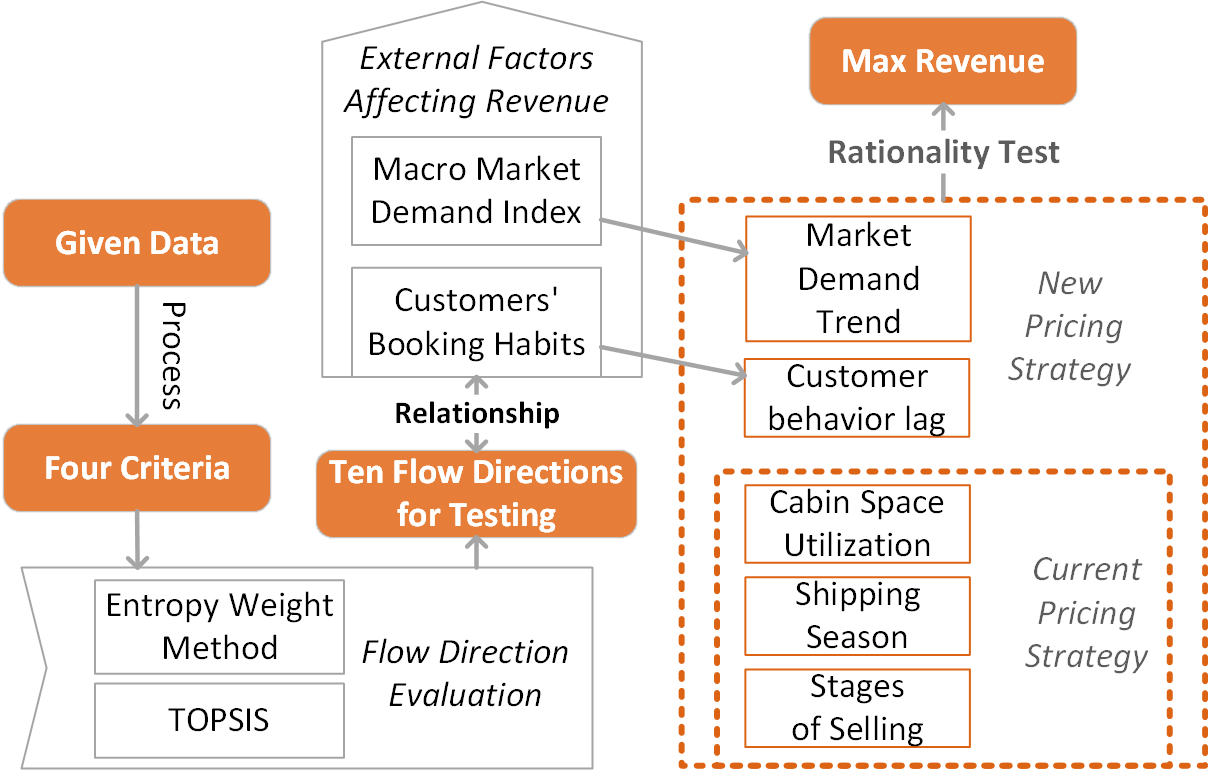
\includegraphics[scale=0.6]{Chapter-Mock/images-Mock/workflow.png}
    \caption{Workflow of Designing Pricing System}
    \label{fig:workflow}
\end{figure}
% We do such things ...
% We begin by establishing a model of ...
\begin{itemize}                %%以圆点方式给出各点
    \item In task 1, we propose four metrics (sales, historical revenue, average freight rate, and port throughput). The Entropy Weight Method is applied to determine the weights. We utilize TOPSIS to implement a comprehensive evaluation and finally select out ten most valuable flow directions for next research.
    \item For task 2(1), we make an analysis on the booking habits of customers. We process the data set to figure out ten violin plots to show the waybill distribution of ten flow directions selected according to the normalized 14-day-long selling period. After that, we apply the algorithm of min-max normalization to discover the evolution trend of the sales volume and the freight rate in one flow direction. We find that customers tend to wait some time after the freight decrease to book the containers.
    \item As to task 2(2), we use Granger Cause Test to study the relationship between the sales volume and the freight rate and get the lag hours related to the former two factors. Additionally, we consider the market demand as an external index and we set a model to calculate it.
    \item As for task 2(3), LSTM is used to predict the market demand index and then to reflect sales volume in short terms. We select three flow directions to make the short-term forecasts and all have satisfactory consequences.
    \item In terms of task 3(1), we make a rationality test to the existing pricing strategy of the shipping company X. We first design a simple pricing strategy to form a basic revenue. Then we simulate the existing pricing strategy, calculate its revenue and define the ratio between these two revenues as the index of rationality.
    \item Regarding task 3(2), we design a new intelligent pricing strategy. We denote a changing rate to control the freight rate change and do the rationality test, which has desired result.
\end{itemize}

% \section{Assumptions and professional explanation}
In order to simplify the problem we are studying, we put the designed dynamic pricing system in an ideal environment. Therefore, we set the following bold assumptions：
\begin{itemize}                %%以圆点方式给出各点
    \item \textbf{Suppose Company X is in a completely monopolistic market and it is only one supplier.}This is an assumption based on Company requirements.
    \item \textbf{The cost is not considered in the container revenue, and only the revenue is calculated as an indicator of maximizing revenue.}This is because the cost composition of the container shipping industry is too complicated, and we made this assumption based on the requirements of Company.
    \item \textbf{Only focus on the containers that are 20 units.} Although there are multiple sizes of containers, we only select the size with a large sample size for analysis, which is a reference for other sizes.
    \item \textbf{Ignore the impact of the contract market on the spot market sales for now.} Due to container inventory constraints, the sales volume of contract orders will affect the spot market orders. But the scheduled time of the contract order may be a year-round cooperation, we cannot learn or predict, so temporarily ignore this influencing factor.
\end{itemize}

Due to the particularity of the container industry, we introduce and define some of its symbol names.
\begin{table}[H]
    \renewcommand\arraystretch{2}   %%控制行间距
    \centering
    \caption{Introduction of Professional words.}
    \begin{tabular}{lll}    %%三列均左对齐
        \toprule  %%表格横线加粗
        \specialrule{0em}{2pt}{2pt}    %%添加透明线控制行高
        Name & Definition  \\
        \specialrule{0em}{2pt}{2pt}    %%添加透明线控制行高
        \midrule
        \specialrule{0em}{1pt}{1pt}
        freight rate & the price of one container \\
        AMT & freight rate\\
        flow direction & a route that only considers the departure and arrival \\
        sales volume & the number of completed container orders \\
        sales & the number of waybills\\
        throughput & an important indicator for measuring port capacity \\
        SVVD & unique identifier of the voyage\\
        ordinary commodities & goods other than special commodities in the spot market\\
        contract market & market with sustained and stable large-scale freight demand\\
        spot market & market with unstable demand and low numbers\\
        \specialrule{0em}{1pt}{1pt}
        \bottomrule
    \end{tabular}
    \label{tbl:Notations}
\end{table}



% %%评价flow direction，挑选出10 valuable flow direction，形式从port_begin到port_end
\section{Task1: Flow Direction Selection}
In this part, we want to filter out ten flow directions with sample value for the pricing system we designed. Because there are contract markets and spot markets in the shipping market, the two influence each other. Our research object is ordinary commodities in the spot market, so we will screen based on the entire market and continue our research.

\subsection {Construct Evaluation System}
We have the following thoughts on the evaluation system for screening flow directions. Since they are used for system testing, they should meet the large number and diversity of samples. Additionally, the ten flow directions should have wealth potential. Therefore, we build an evaluation system as shown in the figure \ref{fig:layer of evaluation}. By using sales volume to reflect the sample size of the flow direction, historical revenue and freight rates to map its wealth potential, and throughput to incarnate its diversity.
\begin{figure}[H]
    \centering
    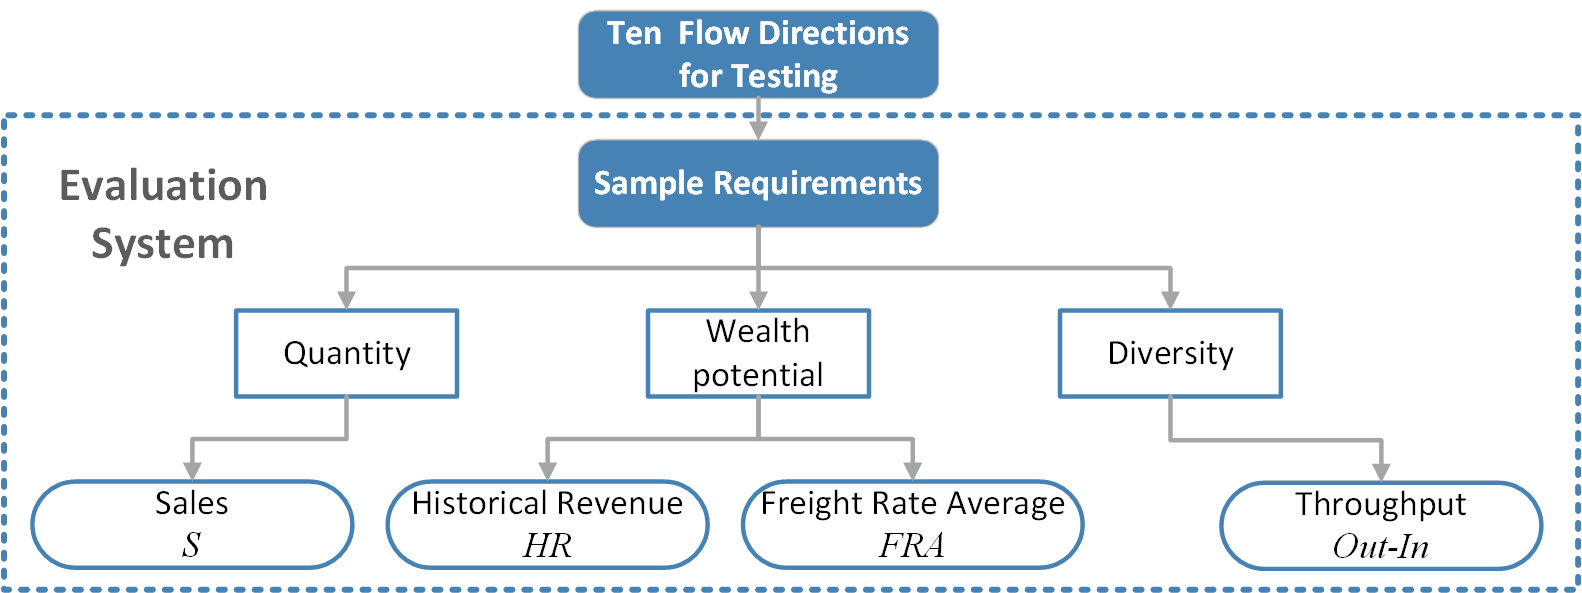
\includegraphics[scale=0.5]{Chapter-Mock/images-Mock/evaluation .png}
    \caption{Evaluation System Structure.}
    \label{fig:layer of evaluation}
\end{figure}

\subsection{Data Processing and Criteria Forming}
The given data set includes 9 properties of the transaction: the ID of one container, the container type, the number of one waybill, the transaction time of one waybill, names of goods, SVVD, AMT (the freight rate), the departure port of the container and the arrival port of the container. In all these properties, we only retain data with containers that are 20 units to simplify the model. And observing these data we find that the freight rate is the same for different goods in the same SVVD at the same time. So we delete the Names of goods and transaction time which are also useless for our evaluation. Then we can obtain the parameters we need according to the following formula definition. 
\begin{itemize}              
    \item Sales ($S$) is the number of waybills. We define the number of container orders as $order\_{quantity}$ (equivalent to sales volume) and the number of times the same waybill is repeated is $repeated\_{counting}$. So we get the formula：
        \begin{equation*}
            S = order\_{quantity} - repeated\_{counting}
        \end{equation*}
   It is noticed that one waybill may include more than one container, so we should delete the repeated counting.
    \item Historical Revenue($HR$) is the sum of the freight rate corresponding to each container, assuming there are $n$ containers in total.
        \begin{equation*}
            HR = \sum_{i=1}^n fr_i
        \end{equation*}
    \item Average Freight Rate($AFR$) is the total revenue divided by the number of orders.
        \begin{equation*}
            AFR = \sum_{i=1}^n fr_i / order\_{quantity}
        \end{equation*}
    \item Port throughput is an important quantitative indicator that reflects the results of port production and operation activities.We define the throughput of the departure port as $Departure_{Ability}$ and the throughput at the arrival port as $Arrival_{Ability}$.The variety of flow directions is directly proportional to both.So We take the average of $Departure_{Ability}$ and $Arrival_{Ability}$ to get $Out\_{in}$ to reflect the throughput.
        \begin{equation*}
            Out\_{in} = \frac{1}{2} (Departure_{Ability} + Arrival_{Ability})
        \end{equation*}
   
\end{itemize}

\subsection{Flow Direction Evaluation}
Following the criteria forming, we will analyze which ten flow directions turns out to be the most valuable ones. In our work, we have designated four criteria based on the data set. The criteria include: HR (Historical Revenue), SV (Sales Volume), AFR (Average Freight Rate), and RA (Region Ability). 

\begin{table}[H]
    \renewcommand\arraystretch{2}   %%控制行间距
    \centering
    \caption{Criteria for Evaluating Flow Direction.}
    \begin{tabular}{cc}    %%三列均左对齐
        \toprule  %%表格横线加粗
        \specialrule{0em}{2pt}{2pt}    %%添加透明线控制行高
        Criteria & Entropy Weight \\
        \specialrule{0em}{2pt}{2pt}    %%添加透明线控制行高
        \midrule
        \specialrule{0em}{1pt}{1pt}
        $HR$ & 0.136367 \\
        $SV$ & 0.652110 \\
        $AFR$ & 0.038062 \\
        $Out\_{in}$ & 0.173461 \\
        \specialrule{0em}{1pt}{1pt}
        \bottomrule
    \label{tbl:Mock-Criteria for Evaluating Flow Direction.}
    \end{tabular}
\end{table}
\vspace{-1cm}

Judging the most valuable flow direction requires melting the above four criteria into a synthetic one. Here we apply \textbf{Entropy Weight Method} to allocate weights to each criterion, and the results are presented in the Table \ref{tbl:Mock-Criteria for Evaluating Flow Direction.}. After that, we utilize \textbf{TOPSIS} (Technique for Order Preference by Similarity to an Ideal Solution) to score each flow direction to filter out the ten flow directions with the highest scores.

\begin{table}[H]
    \renewcommand\arraystretch{2}   %%控制行间距
    \centering
    \caption{TOPSIS Evaluation Results.}
    \begin{tabular}{ccc}    %%三列均左对齐
        \toprule  %%表格横线加粗
        \specialrule{0em}{2pt}{2pt}    %%添加透明线控制行高
        Departure Port & Arrival Port & Score \\
        \specialrule{0em}{2pt}{2pt}    %%添加透明线控制行高
        \midrule
        \specialrule{0em}{1pt}{1pt}
        Yingkou & Ningbo & 0.003902 \\
        Xingang & Nansha & 0.003591 \\
        Yingkou & Nansha & 0.003588 \\
        Yingkou & Fuqing & 0.002518 \\
        Yingkou & Qinzhou & 0.002301 \\
        Yingkou & Shenzhen (Dachan Bay) & 0.001892 \\
        Yingkou & Shantou & 0.001799 \\
        Quanzhou & Yingkou & 0.001709 \\
        Lecong & Yingkou & 0.001592 \\
        Yingkou & Haikou & 0.001574 \\
        \specialrule{0em}{1pt}{1pt}
        \bottomrule
    \label{tbl:Mock-TOPSIS Evaluation Results.}
    \end{tabular}
\end{table}
To conclude, the ten most valuable flow directions are listed in the above table (see in Table \ref{tbl:Mock-TOPSIS Evaluation Results.}) according to the scores by TOPSIS evaluation. Then we mark the departure and arrival ports on the map, complete the direction and finally get the picture of ten flow directions (see in Figure \ref{fig:Mock-flow directions}).
\begin{figure}[H]
    \centering
    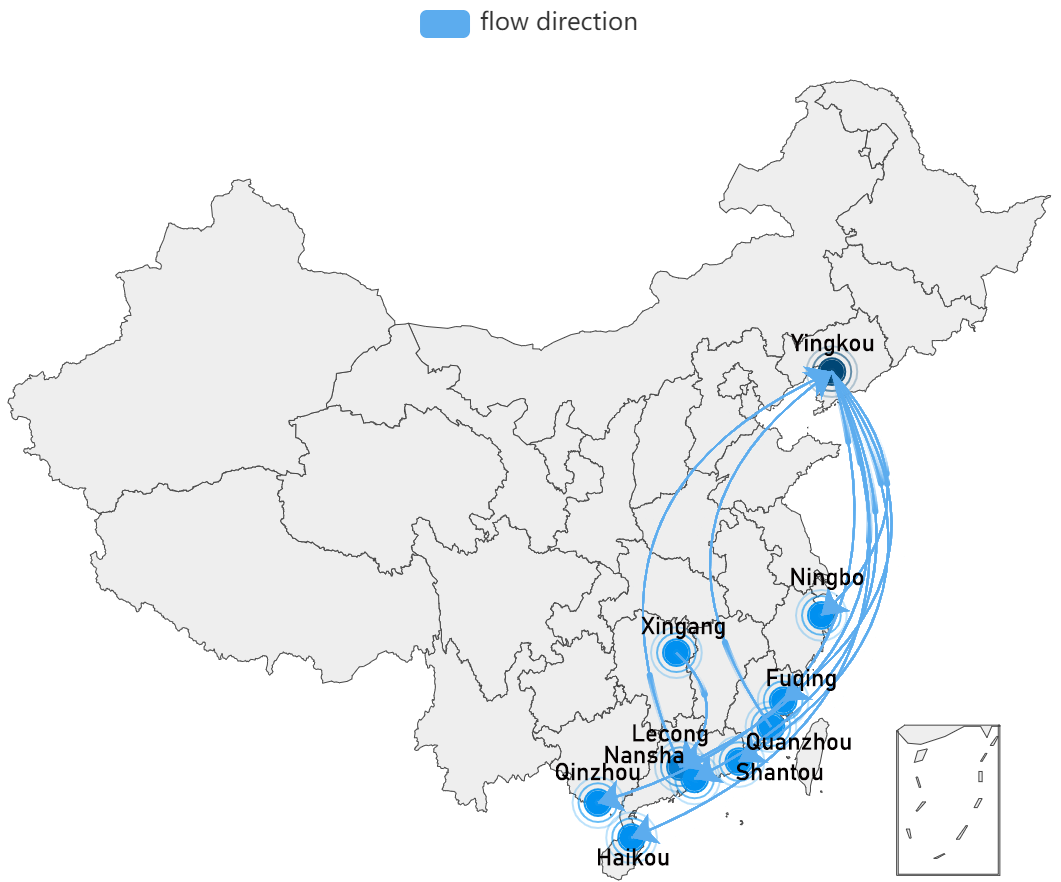
\includegraphics[scale=0.3]{Chapter-Mock/images-Mock/flow directions.png}
    \caption{Flow Directions.}
    \label{fig:Mock-flow directions}
\end{figure}

It can be seen from the table and the figure that almost all ten flow directions contain the city Yingkou, seven in departure ports and two in arrival ports. We believe that coastal routes occupy the main route sample because of its high transaction volume and large value. At the same time, it also contains an inland route, maintaining the diversity of the samples.So far, ten most valuable sample flow directions have been selected.



% \section{Task 2.Research on price influence factors}
Next, we consider how to maximize revenue, which is determined by sales and freight. So we should have a research on the relationship of them firstly. We take into account factors such as customer's booking habits and changes in the macro market that will play a role.

\subsection{Task 2(1). Booking Habits Analysis}

Based on existing facts, we know that the booking habits of customers in each flow direction may be different. For example, customers may prefer to book a container at the end of the sale on a certain flow direction, but may prefer to book the container at the beginning of the sale on another flow direction. Generally speaking, the sales period of the transportation space will start 14 days before departure. So we make a bold conjecture that the difference in customer booking habits may be related to price fluctuations in the spot market.

We implement the following plan and finally get the result in line with our conjecture.

At First, we try to discover the relationship between customer booking habits and flow directions. In order to simplify the problem, we used the previously selected ten routes with sample conditions for analysis.Since we cannot find the actual sales time of the voyage in the data set, we make the following \textbf{assumptions: the first transaction time is regarded as the sales start time, and the last transaction time is regarded as the departure time.} In this way, we can match the transaction time to a natural number, which helps us analyze and draw pictures.

To vividly show the difference of booking habits between different flow directions, we use the data to draw a \textbf{violin plot}.The violin plot (see in Fig. \ref{fig:Mock-booking habits}) takes the ten flow directions as the horizontal axis, and we do the following operations to each flow direction:
\vspace{-0.5cm}
\begin{enumerate}
     \item We use SVVD(S represents route, the first V represents the name of vessel, the second V represents voyage number, D represents direction.) to divide one flow direction into a few voyages.
     \item We count the number of waybills according to the transaction time in each voyage and add them up to get a final result of the flow direction.
     \item We apply the waybill number to the vertical axis of the violin plot, which shows the distribution of waybills from the beginning to the end of the sales.
\end{enumerate}
\begin{figure}[H]
    \centering
    \vspace{-0.8cm}
    \includegraphics[scale=0.15]{Chapter-Mock/images-Mock/booking habits.png}
    \caption{Booking Habits on ten flow directions.}
    \label{fig:Mock-booking habits}
\end{figure}

Through this figure, it is not difficult to find that the booking habits of customers in different directions are diverse. Customers on Xingang-Nansha, Yingkou-Nansha, and Quanzhou-Yingkou flow direction prefer to book at the late of sales period. And the changing trends of Yingkou-Shantou and Yingkou-Haikou flow direction are very similar. But it is difficult to summarize a specific law of booking habits. We can also get the order distribution percentage in the 14-day sales period based on this.

It drives us to explore the reasons behind it, so next we explore the relationship between the price change of ordinary commodities and the sales volume according to the transaction time. We choose the flow direction of Yingkou-Ningbo to continue research because its sales volume outnumbers others' among the 10 flow directions.

Now that different SVVD in the Yingkou-Ningbo flow direction differs in their selling period and freight rate fluctuation, we normalized the data to accomplish the study. We use \textbf{Min-max Normalization} to transfer all the selling period to a general one which is 14 days. Similarly, we standardize the freight rate in an interval from 1000 to 2000. 

%%插入伪代码
\begin{algorithm}[H]
\caption{Min-max normalization}
  \KwIn{Waybill information set $\mathcal{W}$}  
  \KwOut{distribution of waybill order time $\mathcal{T}$, normalized freight rate evolution trend $\mathcal{F}$}  
  Classify all the waybills according to their SVVD.
  
  \For {each waybill class $\mathcal{C}$}
  {  
    Find out the earliest and the latest order time $t_e$, $t_l$ among $\mathcal{C}$.
    
    Find out the highest and the lowest freight rate $r_h$, $r_l$ among $\mathcal{C}$.
    
      \For{each waybill $i$ in $\mathcal{C}$}  
      {  
      
      Normalize its order time $t_i=\frac{t_i-t_e}{t_l-t_e}*14$
      
      Normalize its freight rate $r_i=\frac{r_i-r_l}{r_h-r_l}*1000+1000$
      }  
  }  
  
  Denote the waybill information set after normalization as $\mathcal{W}_n$
    
  Count the normalized order time among $\mathcal{W}_n$ to get $\mathcal{T}$.
  
  Sort $\mathcal{W}_n$ based on their order time to get $\mathcal{F}$.
  
\end{algorithm}

%%时间映射到0-14天，freight rate映射到1000-2000
As for the sales volume, we shift to show the waybill distribution at a smaller time scale, which can directly imply the waybill number at a certain time. After that, we get the following Figure \ref{fig:Mock-The Evolution Trend of Waybill Distribution and Freight Rate} to show the evolution trend of the waybill distribution and the freight rate according to the same 14-day-long selling period.To show clearly, we select one of the sections to be enlarged and present in Figure \ref{fig:Mock-The Evolution Trend of Waybill Distribution and Freight Rate-zoom}

\begin{figure}[H]
    \centering
    \subfigure[Global.]{
    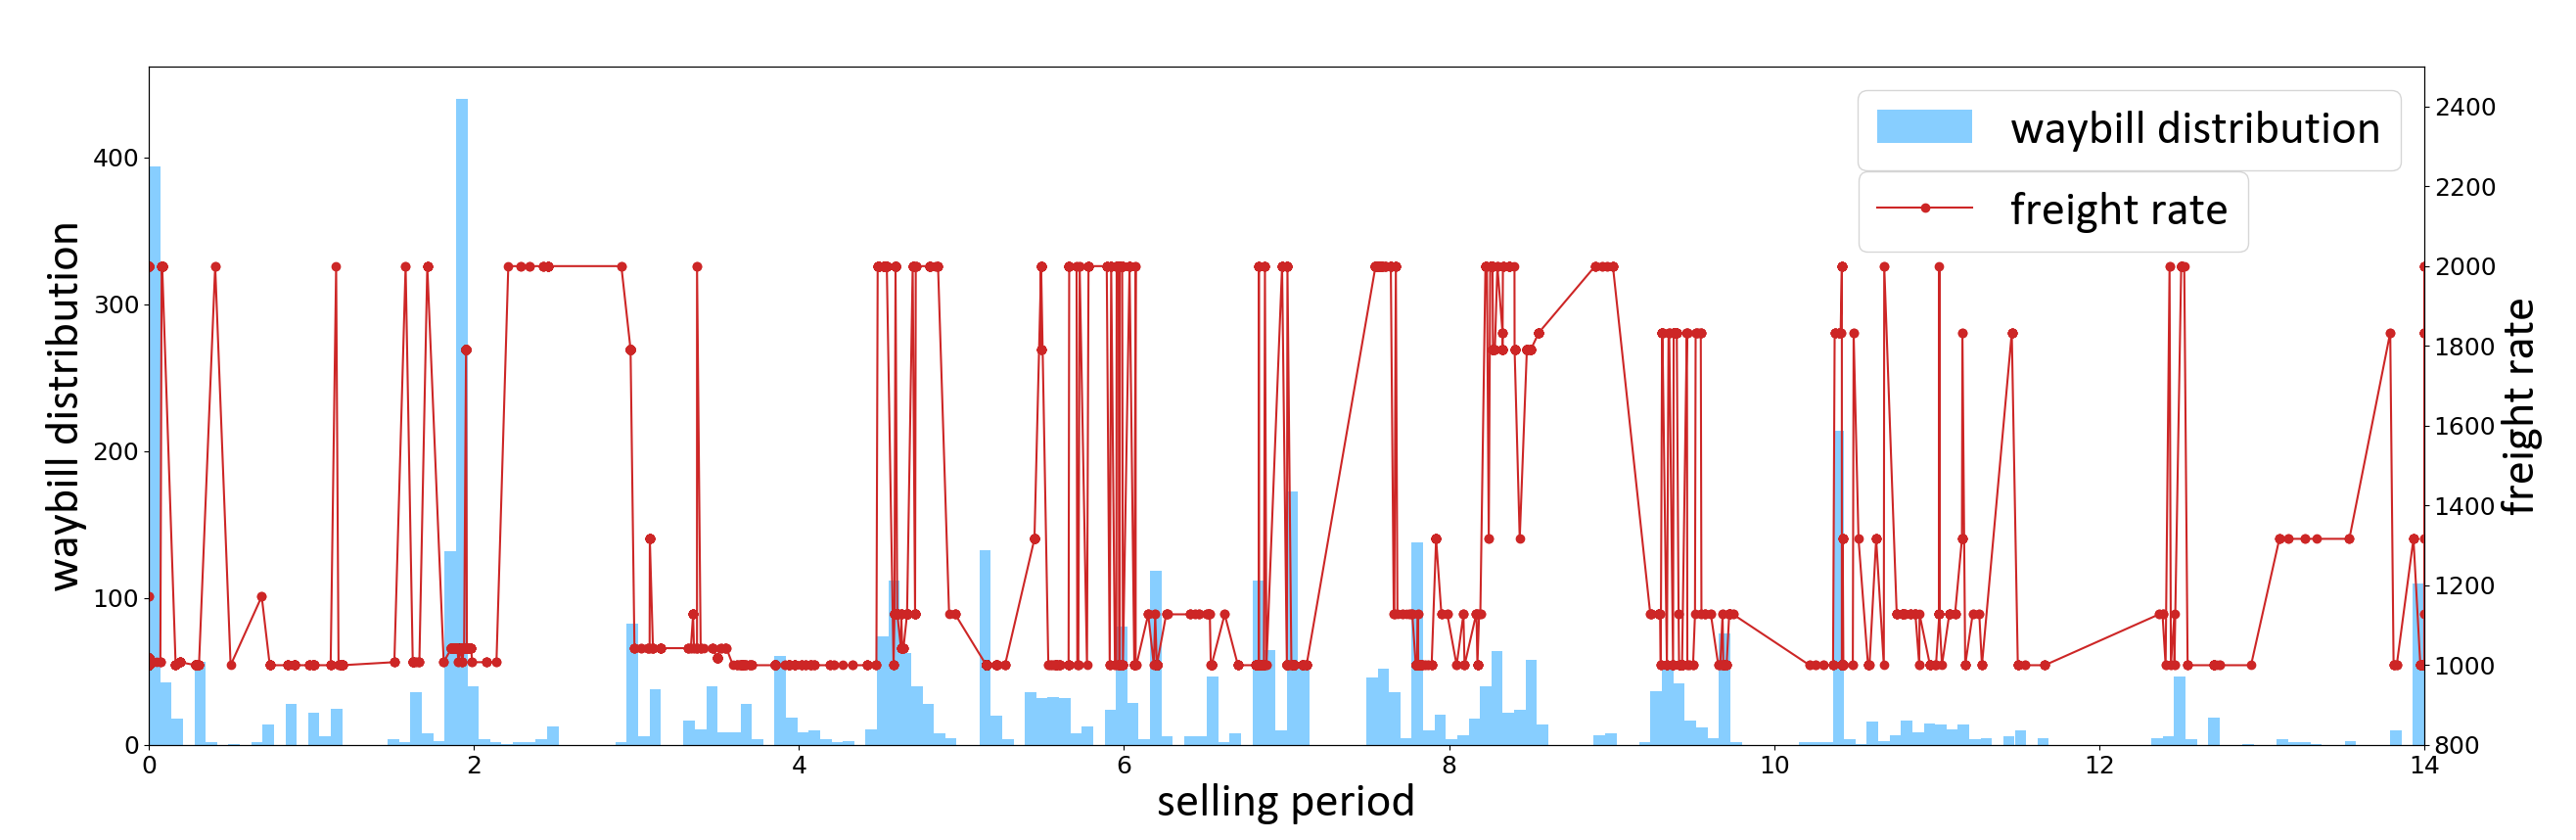
\includegraphics[scale=0.2]{Chapter-Mock/images-Mock/WF-S1.png}
    \label{fig:Mock-The Evolution Trend of Waybill Distribution and Freight Rate}
    }
    \quad
    \subfigure[Partial.]{
    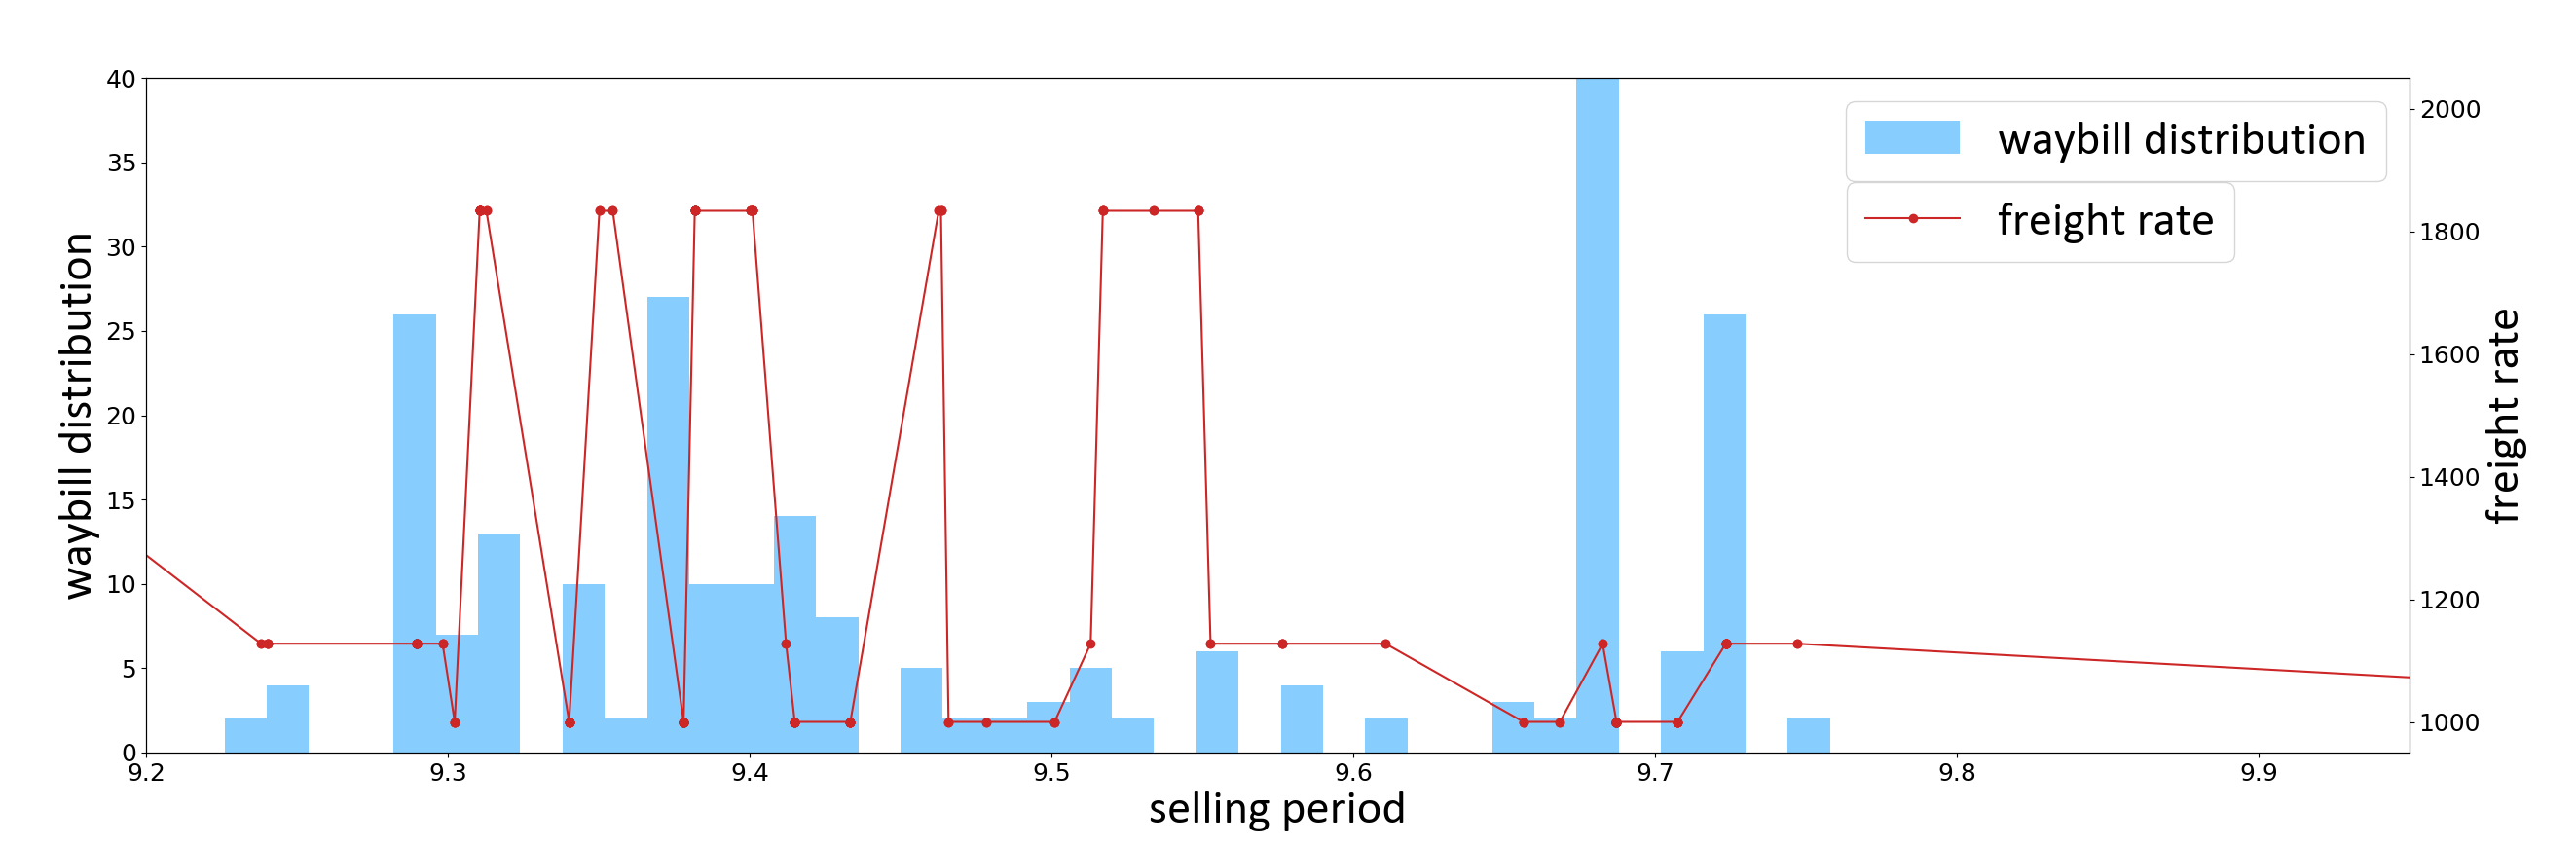
\includegraphics[scale=0.2]{Chapter-Mock/images-Mock/WF-S2.png}
    \label{fig:Mock-The Evolution Trend of Waybill Distribution and Freight Rate-zoom}
    }
    \caption{The Evolution Trend of Waybill Distribution and Freight Rate.}
\end{figure}

It can be concluded from the above research that when the freight is relatively low, customers tend to book containers, and when the freight is high, customers will continue to wait. This behavior indicates that customers are more willing to buy at low prices. These analysis also help us to discover the other relationships in later tasks.

\subsection{Task 2(2). Relationship between Sales Volume and Freight Rate}
\subsubsection{Factors: Booking Habits}
In the previous study, we find that the pattern of customers' booking habits has some relationship \parencite{zym} with the trend of freight rate fluctuation, that is, customers will react to changes in prices and the response has a certain lag. To further dig out which is the lag variable, we apply the \textbf{Granger Cause Test} for causal inference.

Granger Cause Test is a well-known method in Statistics to determine if a particular variable comes after another in the time series and what the lags are. It is a bottom up procedure which assumes the data-generating processes in any time series are independent variables; then the data sets are analyzed to see if they are correlated.
%如何检验要不要详细说明
\begin{table}[H]
    \renewcommand\arraystretch{2}   %%控制行间距
    \centering
    \caption{Granger Causality: Number of lags (no zero) 2}
    \begin{tabular}{cc} 
        \toprule
        \specialrule{0em}{1pt}{1pt}
        ssr based F test & F=2.6948, p=0.0181, df\underline{\hbox to 0.2cm{}}denom=101, df\underline{\hbox to 0.2cm{}}num=6\\
ssr based ch12 test & ch12=18.2498, p=0.0056, df=6\\
likelihood ratio test & ch12=16.9283, p=0.0096, df=6\\
        \specialrule{0em}{1pt}{1pt}
        \bottomrule
    \label{tbl:Mock-Grange Cause Test}
    \end{tabular}
\end{table}
\vspace{-0.8cm}
From the results in Table \ref{tbl:Mock-Grange Cause Test}, we can claim with at least 95 percent confidence level that the order number comes after the freight rate and the lags are 6 data points. As we have divided the 14-day selling period into 120 time slices, this results means that plenty waybill orders often come after decrease in freight rate with lags within 17 hours.%是不是要继续探寻其他流向的反应时间

So far, we can get the conclusion that, on a small time scale, changes in freight rates will greatly affect customer booking behavior and further affect sales volume.The specific manifestation is that when the freight rate increases compared with the previous period, sales will decrease; when the freight rate decreases compared with the previous period, the sales increase, but there is a certain amount of lag in the reaction process.
\subsubsection{Factors: Market Demand}
In addition, we also consider the impact of changes in the macro market on sales and pricing. We \textbf{assume that the demand generated by the market must be realized within the next 14 days}, that is, the customers in need must make the predetermined behavior within the next 14 days. The reason why we choose the 14-day period is that the usual shipping period is 14 days, which not only fully considers the waiting time for customers to order, but also simplifies our model. And the sales period is divided into 14 days.

Here we define the symbol of the market demand index as $M$, and the market demand index on the i\^th day as $M_i$, where $i\in\{0,1,\dots,n \}$. This results in a set of market demand for each day of the sales period. We denote this set by：$$[M_0\quad M_2\quad \dots \quad M_{n}]$$

According to the analysis in task2.(1), we can get the percentage of sales order distribution during the same flow up sales period. Then we define the set by:
$$[a_0\quad a_2\quad \dots \quad a_{13}], subject\quad to \sum_{i=0}^{13}a_i = 1.$$

And we define the sales volume on the i\^th day as $T_j$, where $j\in\{1,2,\dots,n+13 \}$ and  $T_j = 0$, when $j < 14$.
Then there is the following equation：
\begin{equation}
{
    \begin{bmatrix}
        T_{1} & T_{2} & \cdots & T_{14} \\
        T_{2} & \ddots &        & \vdots\\
        \vdots &       & \ddots  &\vdots  \\
        T_{n} & \cdots &\cdots & T_{n+13}
    \end{bmatrix}
}
\times
{\left[
    \begin{array}{cc}
         a_0  \\
         a_1  \\
         \vdots\\
         a_{13}
    \end{array}
\right ]}
=
{\left[
    \begin{array}{cc}
         M_{0}  \\
         M_{1}  \\
         \vdots\\
         M_{n-1}
    \end{array}
\right ]}
\label{eq:Cal market index}
\end{equation}\\
\vspace{-0.1cm}
Next, we can solve $M_0\sim M_{n-1}$ based on the known sales volume data. This means that we can get the history market demand index according to the current sales volume. Then we can use the above algorithm to dig out the market demand index of each flow direction from the data set and show its fluctuation trend over time. We choose three flow directions Yingkou-Ningbo, Xingang-Nansha and Yingkou-Nansha to show in Fig.\ref{Fig:a}.

\begin{figure}[H]
    \centering
    \subfigure[Yingkou-Ningbo.]{
    \begin{minipage}[t]{\linewidth}
    \centering
    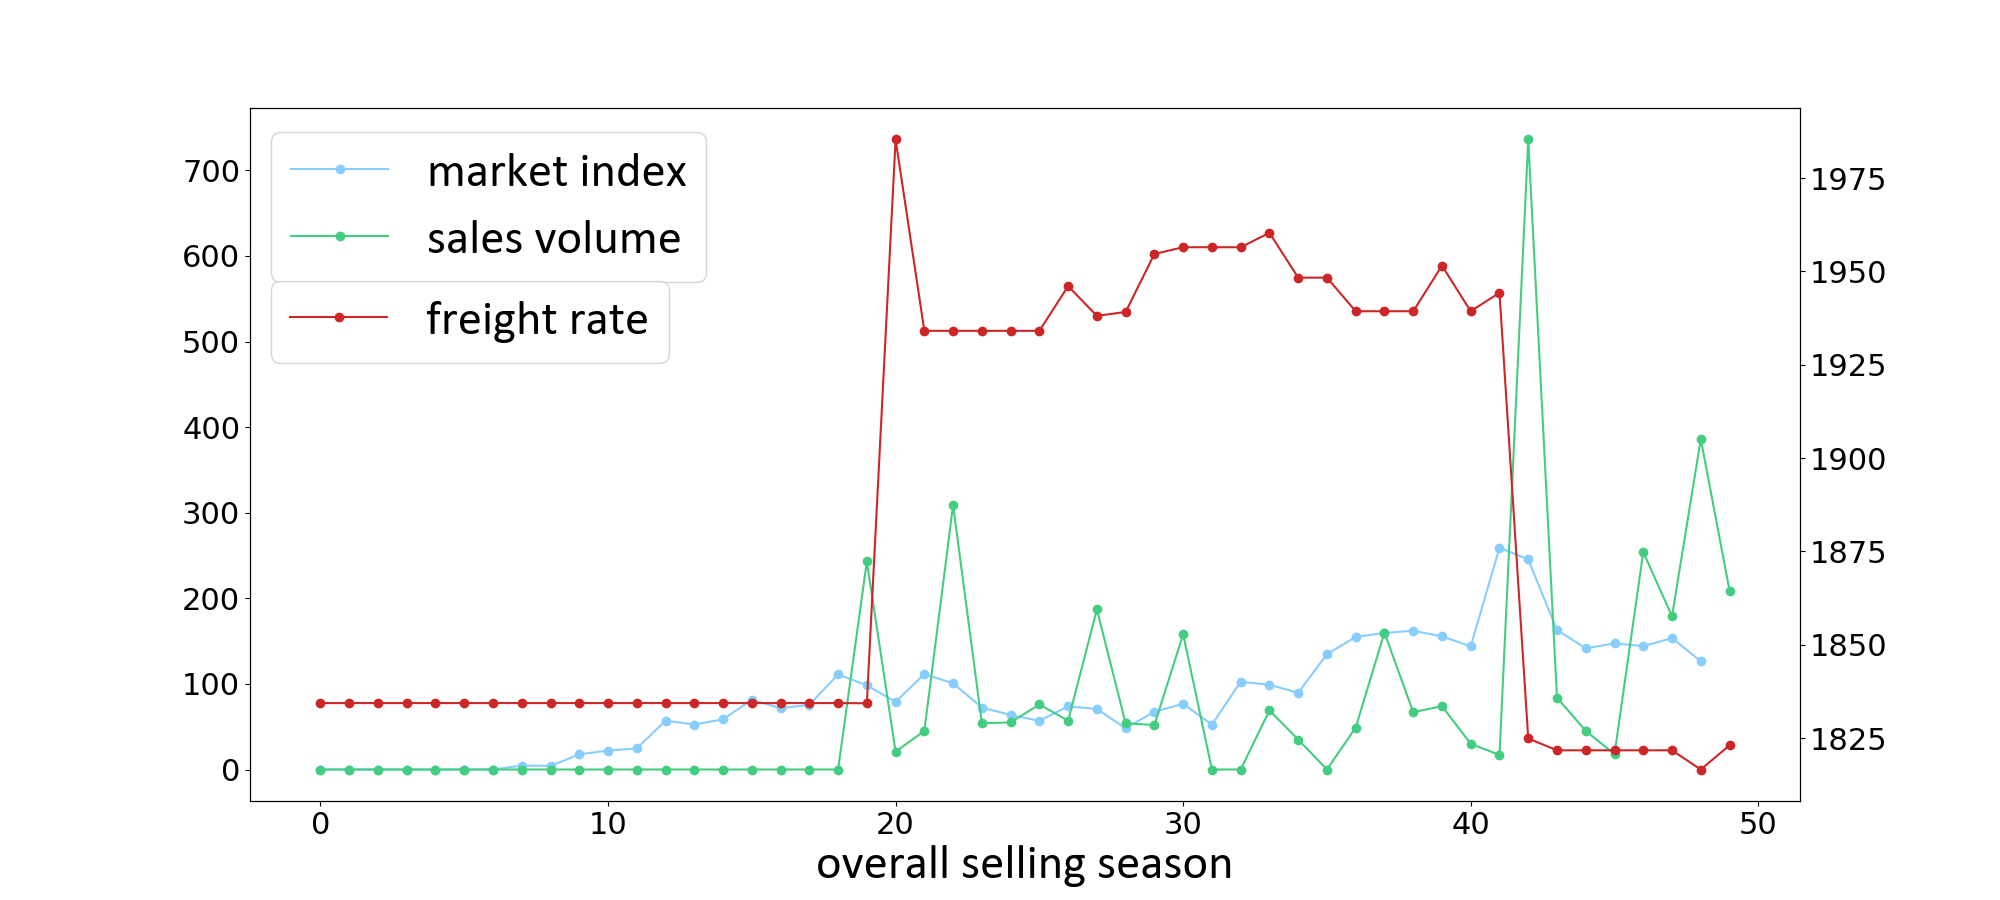
\includegraphics[scale = 0.3]{Chapter-Mock/images-Mock/2_2_1.png}
    \end{minipage}
    }\\
    \subfigure[Xingang-Nansha.]{
    \begin{minipage}[t]{\linewidth}
    \centering
    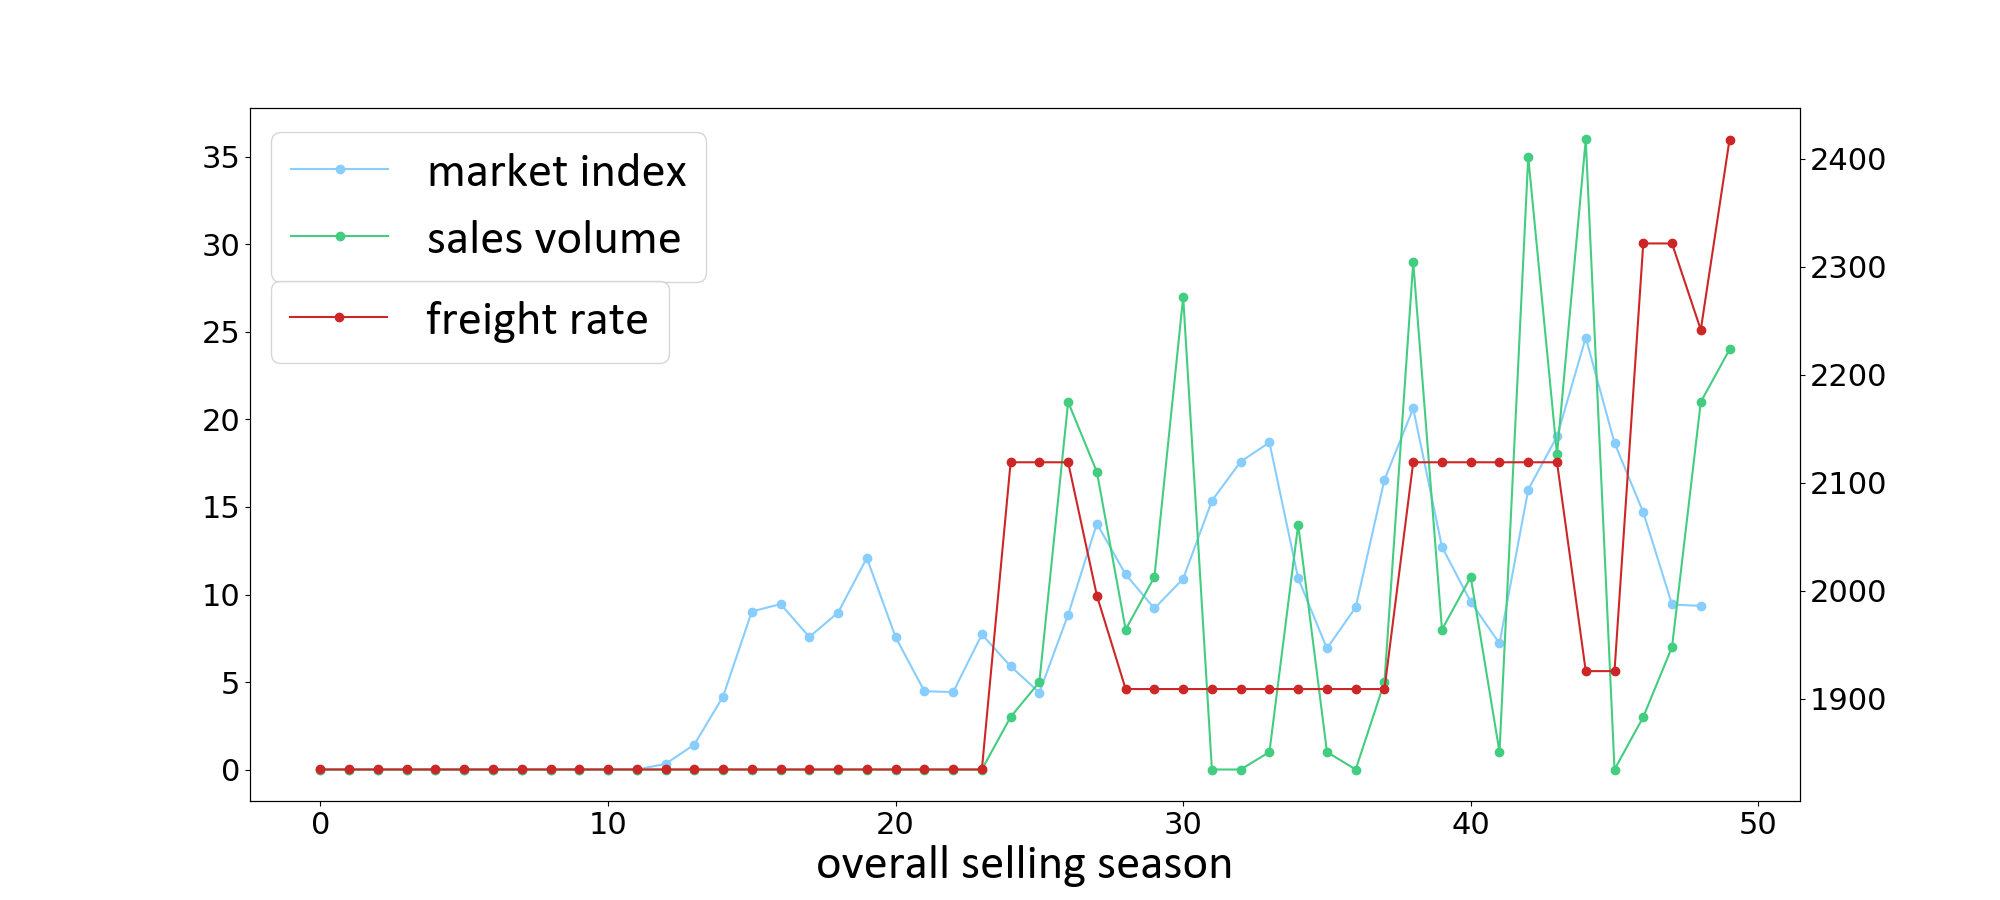
\includegraphics[scale = 0.3]{Chapter-Mock/images-Mock/2_2_2.png}
    \end{minipage}
    }\\
    \subfigure[Yingkou-Nansha.]{
    \begin{minipage}[t]{\linewidth}
    \centering
    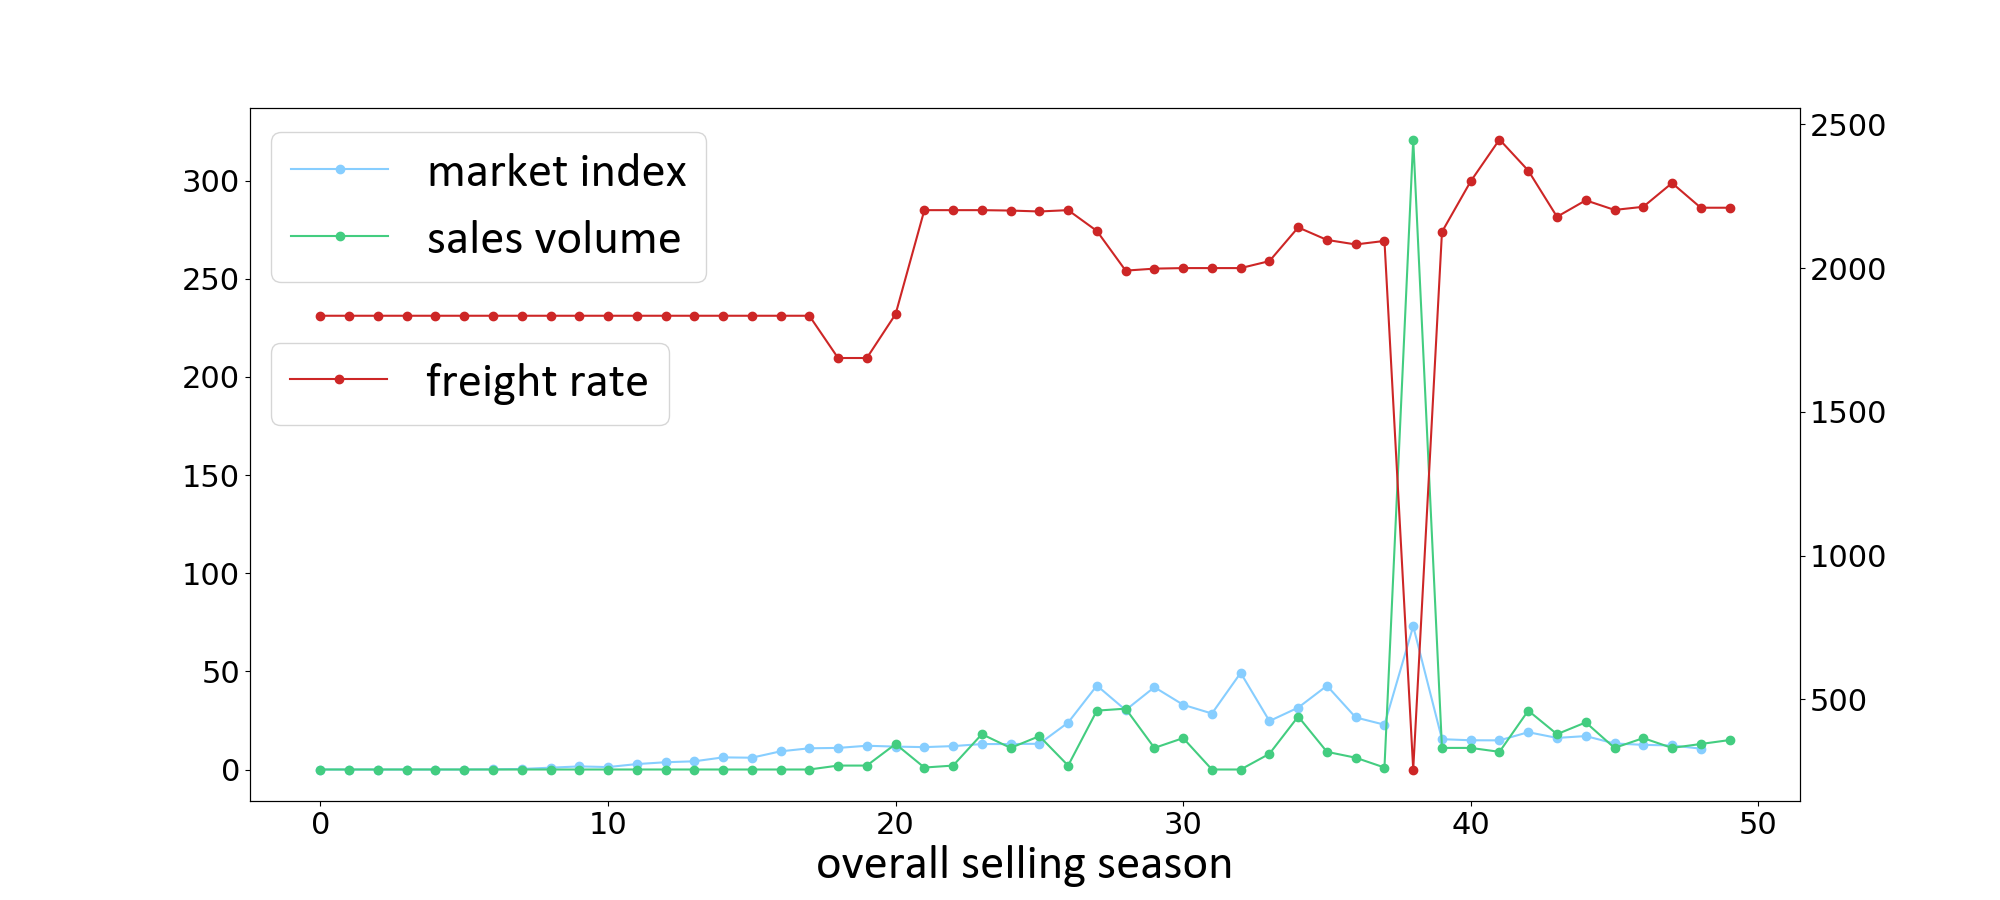
\includegraphics[scale = 0.3]{Chapter-Mock/images-Mock/2_2_3.png}
    \end{minipage}
    }
    \caption{Market demand index fluctuation.}
    \label{Fig:a}
\end{figure}

According to the definition we have made, the market demand index will imply the future sales volume, which means that the correlation between sales volume and market demand is positive. Combined with the changing curve of the freight rate, we find that when the sales volume rises, the freight rate will decrease, and vice versa. There is a negative correlation between the two. Furthermore, we can get such a relationship: the shipping market demand index will positively affect the future sales of containers, and the freight rate will be adjusted according to the sales.

To sum up, we can summarize the relationship between sales volume and freight rate as follows: customers will decide the transaction time due to the freight rate, which is reflected in the sales distribution in a certain selling period; the market demand will affect the future sales volume, and the freight rate will be adjusted  based on sales volume. In short, the freight rate will affect the sales volume, and the sales volume will also influence the freight rate.

\subsection{Task 2(3). Prediction of Market conditions}
In the above analysis, we obtain the value of the market demand index and get its volatility curve over time. From this analysis, we grasp the influence of changes in market demand on sales, which is conducive to the pricing of freight rates. Therefore, a short-term forecast of market conditions is very beneficial to the design of the next pricing system.

In this regard, we tend to reflect future market trends by forecasting sales volume. We use Long and Short-Term Memory (LSTM)  to make a prediction of sales volume based on existing time series data\parencite{2016LSTM}.

LSTM model  is a variant of recurrent neural network (RNN). It is well-suited to classifying, processing and making predictions based on time series data. A common LSTM unit is composed of a cell, an input gate, an output gate and a forget gate. The cell remembers values over arbitrary time intervals and the three gates regulate the flow of information into and out of the cell\parencite{lstm1}.

Some specific applying details of the model:

\begin{enumerate}[\quad\bf1.]
\item Input and Output

We first group the market demand index sequence three at a time to construct a training matrix, and then label each of them with the exact index coming right after them. Therefor, our input of the model is a 3-dimension index sequence and the output of the model is one predicted index. 
\item Loss Function

During the training, we use mean square error (MSE) as the loss function:
\begin{equation}
    MSE(x, \hat{x})=\frac{1}{N}\sum_{i=1}^N (x_i-\hat{x_i})^2
\end{equation}

where $x$ is the true target vector and $\hat{x}$ is the predicted feature vector and $N$ is the number of dimension.

\item Training parameters

The number of units of LSTM layer is set to 200 and the whole model contains 482,601 trainable parameters. Our model is trained for 100 epochs with ADAM optimizer.
\end{enumerate}

\begin{table}[H]
    \renewcommand\arraystretch{2}   %%控制行间距
    \centering
    \caption{Prediction model summary}
    \begin{tabular}{ccc}    %%三列均左对齐
        \toprule  %%表格横线加粗
        \specialrule{0em}{2pt}{2pt}    %%添加透明线控制行高
        Layer (Type) & Output Shape & Param \\
        \specialrule{0em}{2pt}{2pt}    %%添加透明线控制行高
        \midrule
        \specialrule{0em}{1pt}{1pt}
        LSTM & (None, 200) & 161600 \\
        Repeated Vector & (None, 1, 200) & 0 \\
        LSTM & (None, 1, 200) & 320800 \\
        Time Distributed & (None, 1, 1) & 201 \\
        \specialrule{0em}{1pt}{1pt}
        \bottomrule
    \label{tbl:Mock-LSTM summary.}
    \end{tabular}
\end{table}
\vspace{-0.8cm}

We select partial sequence from three flow directions to make short-term forecasts and compare the results with raw data. With the predicted market demand index, we can compute the future sales volume using formula \ref{eq:Cal market index}.

\begin{figure}[H]
    \centering
    \subfigure[Yingkou-Ningbo.]{
    \begin{minipage}[t]{0.3\linewidth}
    \centering
    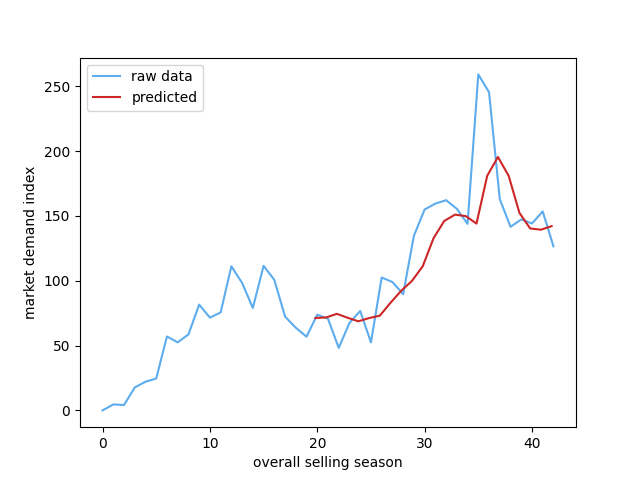
\includegraphics[scale = 0.3]{Chapter-Mock/images-Mock/LSTM_market.png}
    \end{minipage}
    }
    \subfigure[Xingang-Nansha.]{
    \begin{minipage}[t]{0.3\linewidth}
    \centering
    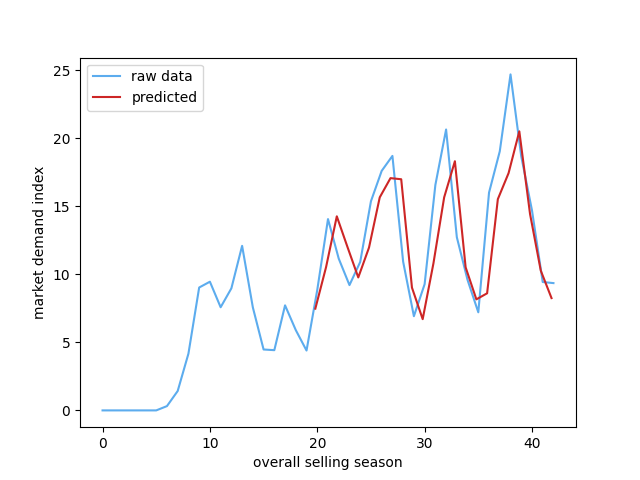
\includegraphics[scale = 0.3]{Chapter-Mock/images-Mock/LSTM_market_2.png}
    \end{minipage}
    }
    \subfigure[Yingkou-Nansha.]{
    \begin{minipage}[t]{0.3\linewidth}
    \centering
    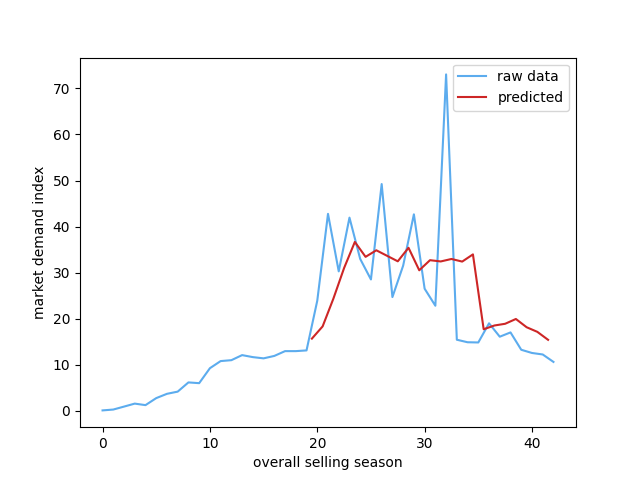
\includegraphics[scale = 0.3]{Chapter-Mock/images-Mock/LSTM_market_3.png}
    \end{minipage}
    }
    \caption{Short-term forecasts of Market Demand Index using LSTM}
    \label{Fig:Short-term of Sales Volume using LSTM}
\end{figure}


\begin{figure}[H]
    \centering
    \subfigure[Yingkou-Ningbo.]{
    \begin{minipage}[t]{0.3\linewidth}
    \centering
    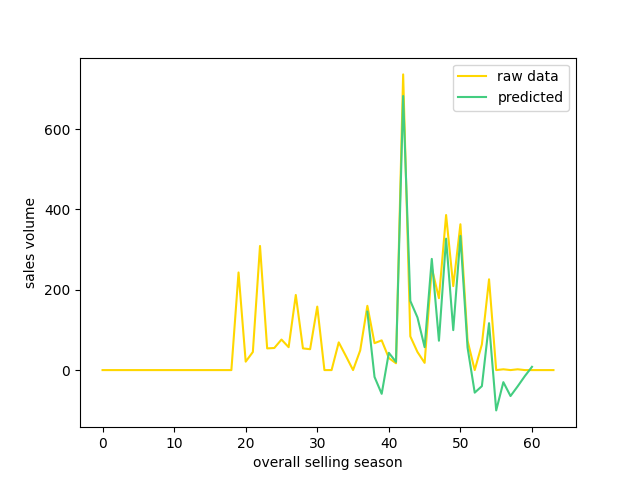
\includegraphics[scale = 0.3]{Chapter-Mock/images-Mock/LSTM_sale.png}
    \end{minipage}
    }
    \subfigure[Xingang-Nansha.]{
    \begin{minipage}[t]{0.3\linewidth}
    \centering
    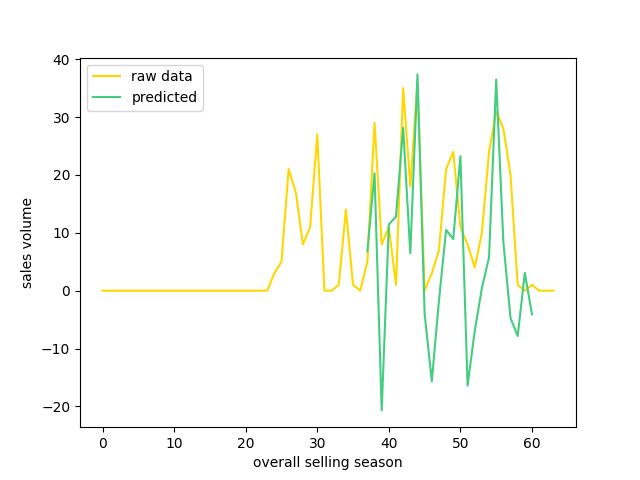
\includegraphics[scale = 0.3]{Chapter-Mock/images-Mock/LSTM_sale_2.png}
    \end{minipage}
    }
    \subfigure[Yingkou-Nansha.]{
    \begin{minipage}[t]{0.3\linewidth}
    \centering
    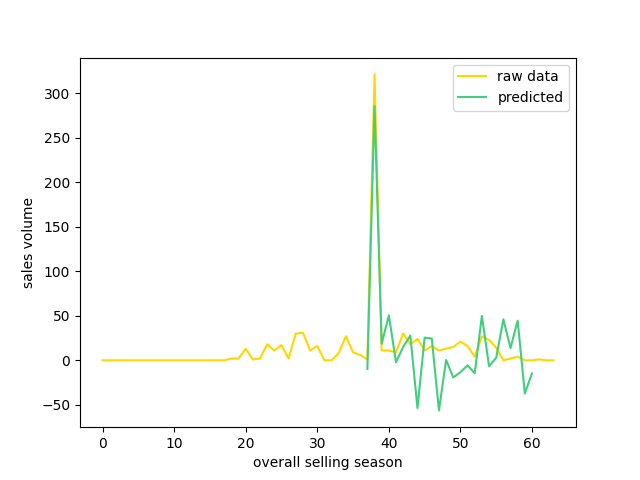
\includegraphics[scale = 0.3]{Chapter-Mock/images-Mock/LSTM_sale_3.png}
    \end{minipage}
    }
    \caption{Sales volume calculated by prediction}
    \label{Fig:Sales volume calculated by prediction}
\end{figure}

As shown in Fig. \ref{Fig:Short-term of Sales Volume using LSTM}, the market demand of Yingkou-Ningbo and Yingkou-Nansha will meet a small peak according to raw data and is correctly predicted by our model. As for Xingang-Nansha, our model have predicted exact the same fluctuation with raw data. In Fig. \ref{Fig:Sales volume calculated by prediction}, the sales volume caculated by our prediction matches raw data well, which means that our model is reasonable for the prediction of sales volume and can be further applied in the following study. 






% \section{Task3. Pricing Strategy}

After studying the characteristics and relationship between the several indexes, we begin to investigate what an intelligent pricing strategy \parencite{psgxr} \parencite{wtl}should be like. In this section, we first value the rationality of the existing pricing strategy and then design a new dynamic pricing strategy based on what we have done before. At last, we also make a rationality test of the new pricing strategy, which proves to be effective.

\subsection{Task3(1). Rationality Test of the Existing Pricing Strategy}

In this section, we are going to test the rationality of the existing pricing strategy.

At first, We assume a simple pricing strategy: the one that keeps a stable freight rate. The revenue produced by this simple strategy will be used as a baseline to measure the rationality of other strategies. 

To calculate the total revenue, we first make efforts to simulate the sales volume. Take the flow direction of Yingkou-Shantou in the peak season as an example. We calculate the average market index of the flow direction through the way same as section 4.2.2 and then use the average to allocate the sales volume with initial value.

We dynamically adjust the sales volume fluctuation based on the lag time we have done in section 4.2.1 according to freight rate. At the same time, we change the freight rate as long as the space utilization reaches the threshold value according to the existing strategy of Company X. Then we compose the sales volume and freight rate to get the whole revenue, which is denoted as $Revenue_{Existing}$.

Similarly, we use the same technique to calculate the revenue of the simple pricing strategy of Company X, which is denoted as $Revenue_{Basic}$. We denote the ratio as the rationality through 

\begin{equation*}
    Rationality_{Existing} = \frac{Revenue_{Existing}}{Revenue_{Basic}}
\end{equation*}

The bigger the ratio is, the more rational the pricing strategy is.

\begin{figure}[H]
    \centering
    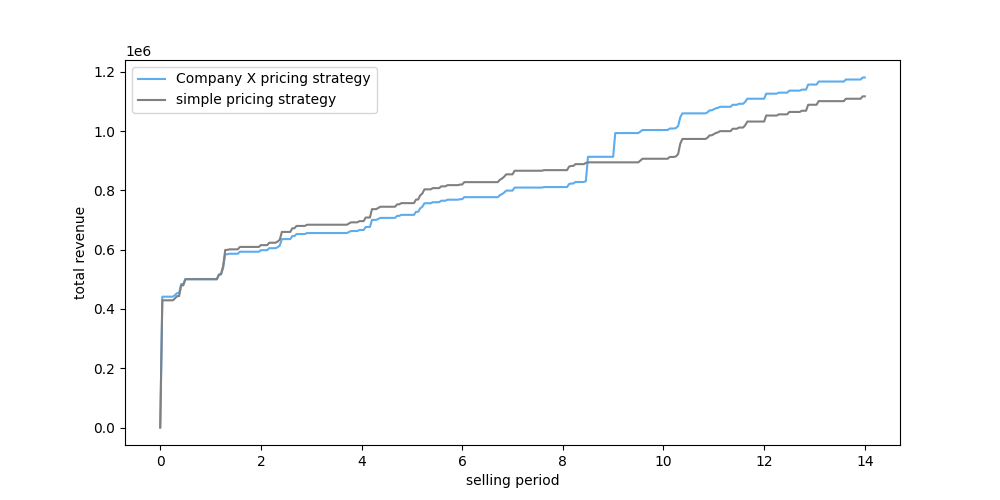
\includegraphics[scale=0.5]{Chapter-Mock/images-Mock/3_1.png}
    \caption{Rationality test of the existing pricing strategy.}
    \label{fig:Mock-Rationality-Existing}
\end{figure}

Seeing from the figure \ref{fig:Mock-Rationality-Existing}, we can conclude that the existing pricing strategy of the shipping company X has its rationality.

\subsection{Task3(2). Design of the Intelligent Pricing Strategy}

In order to achieve the goal of the shipping company X to maximize the revenue, we start to design and formulate a smarter and more reasonable pricing strategies.

Our design is shown in the following steps.
\begin{enumerate}[\quad\bf1.]
\item We make an assumption in our pricing strategy firstly, which is the entire selling periods of different SVVDs are all the same 14 days. Although the sales period of each voyage is different, we follow the 14-day sales period under popular conditions, which makes our model universal. Then we divide the 14-day sales period into $n$ extremely small sales time units.

\item Simple explanation for the pricing strategy

\hspace{1em}
We denote current freight Rate ($CFR$) and changing rate ($CR$) as two basic indexes to measure and change the freight rate. The notation of $CFR$ tends to directly show the current freight rate, which can be seen by customers. Meanwhile, $CR$ is defined to control the change of the freight rate precisely and timely, which is calculated by the pricing strategy and cannot be seen by customers.

\hspace{1em}
We suppose that the pricing strategy will automatically calculated the $CR$ in each sales time units based on the data and then change the $CFR$ according to the formula and objective function that we set in the pricing strategy.

\item Details and Formulas in the pricing strategy

\hspace{1em}
As for $CFR$, we set an initial freight rate, which is denoted as $CFR_0$. Now that $CFR$ will change in a stable interval, we denote the $CFR$ in the $i^{th}$ time unit  as $CFR_i$, where $i\in\{0,1,\dots,n \}$. Similarly, the $i^{th}$ $CR$ is also denoted as $CR_i$. However, the value of $CFR_0$ needs further discussion. Observing historical data, we know that freight rate fluctuations are small fluctuations within a certain range.So we average the historical price to determine the initial price $CFR_0$.

\hspace{1em}
In terms of $CR$, we combine what we have done together to form a complete influencing factor system.

\hspace{1em}
Firstly, we determine how booking habits affect the $CR$. As we have discussed in Task 2(2), plenty waybill orders often come after decrease in freight rate with lags within 17 hours. This may implies the sensitivity of customers to the freight rate decrease. For example, customers in one flow direction may immediately book the container after noticing a slight decrease on the freight rate, while customers in the other flow direction may patiently wait to book the container until the decrease achieves their ideal level. Such behavior difference can be measured by the lag hours in Task2(2) Granger Cause Test, and here we denote the lag hours as $time_{lag}$. From Task 2(2), we have ten lag hours from $time_{lag}^1$ to $time_{lag}^{10}$ and we can find the maximum which is $time_{lagmax}$. Then we can get the first influencing factor, which we denote as 
\begin{equation*}
    SSTV_i = \frac{time_{lag}^i}{time_{lagmax}}
\end{equation*}
where $i = 1,2,\dots,10$. $SSTV_i$ implies customers' sensitivity to freight rate decrease in the $i^{th}$ flow direction. The bigger $SSTV_i$ is, the more likely it is for customers to wait longer time for a bigger freight rate decrease.

\hspace{1em}
Secondly, we consider the effect of space utilization rate. It is easy to know that higher space utilization rate brings higher revenue. We decide to use $CSUR_i^k$ to symbolize the current space utilization rate of the $k^{th}$ flow direction in the $i^{th}$ selling period. We can get $CSUR_i^k$ through 
\begin{equation*}
    CSUR_i^k = \frac{CurrentUsed}{Total}
\end{equation*}
where $CurrentUsed$ is the number of used containers until the $i^{th}$ selling period and $Total$ is the entire container number of $k^{th}$ flow direction. If $CSUR$ is too low, it will be urgent for the company to decrease the freight rate to appeal to more customers.

\hspace{1em}
Thirdly, we talk about the influence of the selling period stage. Suppose we divide the 14-day-long selling period into $N$ small intervals. Then we can get the current selling period stage through 
\begin{equation*}
    CSPS_i^n = 1-\frac{i}{N}
\end{equation*}
where $i = 1,2,\dots,N$ and $n = 1,2,\dots,10$. With the approaching of departure time, $CSPS$ will become smaller to 0 and means that it is more necessary to care about the empty container.

\hspace{1em}
Fourth, we take the market demand into account. In the way similar to the operation on booking habits, we calculate the ratio between the market demand of the $i^{th}$ selling period $MD_i$ and the overall maximum market period $MD_max$. Then we get the current market demand through 
\begin{equation*}
    CMD_i = \frac{MD_i}{MD_max}
\end{equation*}


\item Construction of $CR$ with the influencing factors 

\hspace{1em}
In the former part, we have discussed the four indexes that affect $CR$ and analyze them to get the same principle that the bigger the index is, the less likely it is for the shipping company to decrease the freight rate. Since these four indexes have the same evaluation meaning, we use \textbf{Analytic Hierarchy Process} (AHP) to decide their weights and achieve a new index $CR$.

\hspace{1em}
To begin with, construct the judgment matrix of $CR-P$: Compare the four factors in pairs to get the judgment matrix (see in Figure \ref{fig:Judgment matrix of CR-P}).

% \begin{table}[H]
%     \renewcommand\arraystretch{2}   %%控制行间距
%     \centering
%     \begin{tabular}{ccccc}    %%三列均左对齐
%         \toprule  %%表格横线加粗
%         \specialrule{0em}{2pt}{2pt}    %%添加透明线控制行高
%          & $SSTV$ & $CSUR$ & $CSPS$ & $CMD$ \\
%         \specialrule{0em}{2pt}{2pt}    %%添加透明线控制行高
%         \hline
%         \specialrule{0em}{1pt}{1pt}    %%添加透明线控制行高
%         $SSTV$ & 1.0000 & 0.5000 & 4.0000 & 0.2500 \\
%         $CSUR$ & 2.0000 & 1.0000 & 2.0000 & 0.5000 \\
%         $CSPS$ & 0.2500 & 0.5000 & 1.0000 & 0.2000 \\    
%         $CMD$ & 4.0000 & 2.0000 & 5.0000 & 1.0000 \\
%         \specialrule{0em}{1pt}{1pt}    %%添加透明线控制行高
%         \bottomrule
%     \end{tabular}
%     \caption{Judgment matrix of $CR-P$.}
%     \label{tbl:Judgment matrix of CR-P}
% \end{table}

\begin{figure}[H]
    \centering
    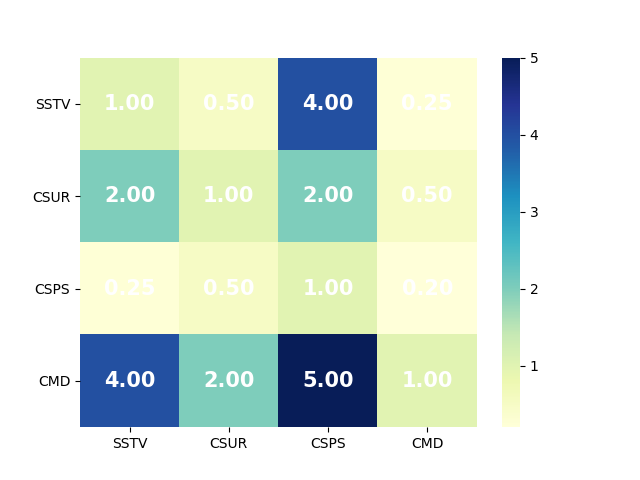
\includegraphics[scale=0.8]{Chapter-Mock/images-Mock/AHP.png}
    \caption{Judgment matrix of $CR-P$.}
    \label{fig:Judgment matrix of CR-P}
\end{figure}

\hspace{1em}
%%计算特征值，权重向量
%%代码见python
After that, it is easy to solve the eigenvalues of the matrix $CR-P$ and get the weight vector is $\omega_i = {(0.1701,0.2406,0.0805,0.5088)}^T$.

\hspace{1em}
Now we make the consistency check.

\hspace{1em}
Since the consistency index $CI = \frac{\lambda_{max}-n}{n-1}$ and the consistency ratio $CR = \frac{CI}{RI}$, where $RI$ is only relative to the matrix size (see in Table \ref{tbl:Mock-The value of RI}).

\hspace{1em}
By calculating, we get $CR = 0.0786<0.1$, which passes the consistency check.

%%The value of RI
\begin{table}[H]
    \renewcommand\arraystretch{2}   %%控制行间距
    \centering
    \begin{tabular}{ccccccccc}    %%三列均左对齐
        \toprule  %%表格横线加粗
        \specialrule{0em}{2pt}{2pt}    %%添加透明线控制行高
        matrix size & 2 & 3 & 4 & 5 & 6 & 7 & 8 & 9 \\
        \specialrule{0em}{2pt}{2pt}    %%添加透明线控制行高
        \hline
        \specialrule{0em}{1pt}{1pt}    %%添加透明线控制行高
        $RI$        & 0 & 0.58 & 0.90 & 1.12 & 1.24 & 1.32 & 1.41 & 1.45  \\
        \specialrule{0em}{1pt}{1pt}    %%添加透明线控制行高
        \bottomrule
    \end{tabular}
    \caption{The value of $RI$.}
    \label{tbl:Mock-The value of RI}
\end{table}

\hspace{1em}
To conclude, we can get the following $CR$ formula as 
\begin{equation*}
    CR = 0.1701\times SSTV+0.2406\times CSUR+0.0805\times CSPS+0.5088\times CMD
\end{equation*}

\item How $CR$ control the change of $CFR$

\hspace{1em}
After the data practice, we find the most intelligent pricing strategy with several indexes determined to maximize the revenue.

\hspace{1em}
For each selling period, we first calculate the present $CR$ and determine the freight rate change through the following way:

We design two different proposals to tackle different pricing strategy of peak season and off season.

\hspace{1em}
As for the $i^{th}$ selling period in the peak season,
\begin{equation*}
    CFR_{i+1} = \begin{cases}
    CFR_i+50\times\frac{CR_i-0.4}{0.4} & , \text{if } CR \geq 0.4; \\
    CFR_i-100\times\frac{0.4-CR_i}{0.4} & , \text{if } CR < 0.4.
    \end{cases}
\end{equation*}

\hspace{1em}
Similarly, the formula in the off season is
\begin{equation*}
    CFR_{i+1} = \begin{cases}
    CFR_i+20\times\frac{CR_i-0.6}{0.6} & , \text{if } CR \geq 0.6; \\
    CFR_i-150\times\frac{0.6-CR_i}{0.6} & , \text{if } CR < 0.6.
    \end{cases}
\end{equation*}
\hspace{1em}
To directly show the principle of our intelligent pricing strategy, we make the following framework of our algorithm in Figure \ref{fig:Intellignet pricing system}.

\begin{figure}[H]
    \centering
    %\vspace{-0.8cm}
    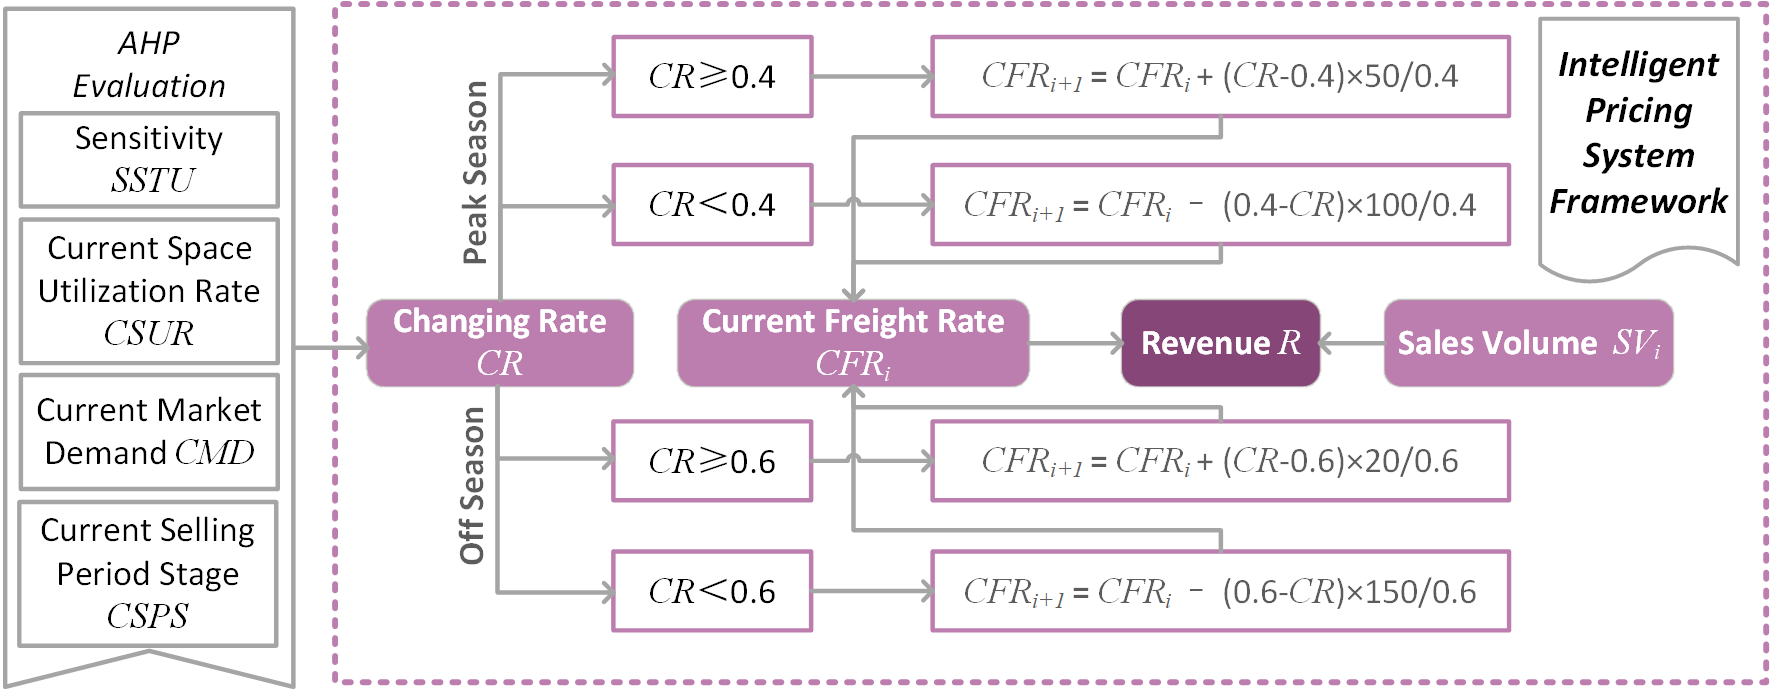
\includegraphics[scale=0.4]{Chapter-Mock/images-Mock/Intelligent Pricing System.png}
    \caption{Intelligent pricing system framework.}
    \label{fig:Intellignet pricing system}
\end{figure}

\item Rational Test

\hspace{1em}
Same as the former part 3.1, we do the rational test to the intelligent pricing strategy and get the following figure \ref{fig:Mock-Rationality-Intelligent}.

\begin{figure}[H]
    \centering
    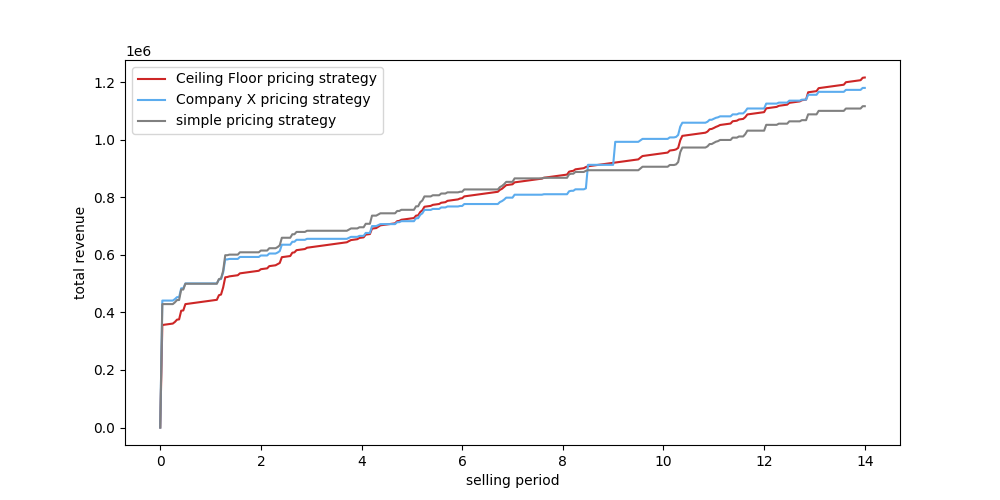
\includegraphics[scale=0.6]{Chapter-Mock/images-Mock/3_2.png}
    \caption{Rationality test of the intelligent pricing strategy.}
    \label{fig:Mock-Rationality-Intelligent}
\end{figure}

\hspace{1em}
We notice that the curve of the intelligent pricing strategy is increasing more smoothly and its revenue is slightly bigger than the one of the existing pricing strategy.From this we can draw our conclusion that the model we designed is superior to the existing pricing strategy.

\end{enumerate}

% \section{Conclusions}
Intelligent dynamic pricing strategy under the background of big data analysis is indispensable in shipping container industry. Our team has drawn the following conclusions when designing pricing strategy based on existing data.
\begin{itemize}
    \item We select ten flow directions based on historical revenue, order quantity, freight rate, and throughput. The results are presented in Table \ref{tbl:Mock-TOPSIS Evaluation Results.}.These ten samples are proved to be meaningful and helpful in the research process.
    \item The time distribution of customers in different flow directions for ordering containers is diverse. The reason behind this is that customers will consider buying according to the rise and fall of the freight rate, thus reflecting the negative correlation between sales volume and shipping rate.
    \item Fluctuations in market demand will affect sales volume and further influence changes in freight rates.
    \item The current pricing strategy is beneficial to increase revenue, but it has limitations due to insufficient considerations.
    \item We design a pricing system to determine whether to adjust the price and the extent of the price adjustment based on the threshold, and test its rationality, and achieved very satisfactory results.
\end{itemize}

However, due to the lack of data and the pressing time, we made many bold assumptions before conducting this research. Furthermore, our future work can be realized when conditions permit.
\begin{itemize}
    \item If we can get the order statistics of the contract market for a long time, we can know the container sales volume generated by the contract market in the short term, and predict the sales volume in the spot market more accurately when the inventory constraints are known\parencite{dynamic-pricing}.
    \item It is more realistic and valuable to maximize the benefits under the consideration of costs. If we can know the composition of container transportation costs, this step can be achieved by us.
\end{itemize}

% \section{Strengths and Weaknesses}

\subsection{Strengths}
\begin{enumerate}[\quad\bf1.]        %%列出1、2、3点
    \item \textbf {Data processing.} We process the data by the algorithm of min-max normalization to transfer all selling period of different length to 14-day-long one. It facilitates our model design and result calculation.
    \item \textbf {Visualization.} We vividly and diversely visualize the waybill distribution by violin plots and use line chart to show the short-term forecasts. Additionally, we integrate line chart and bar chart together to display the evolution trend of the sales volume and the freight rate to further investigate the relationship between them.
    \item \textbf {Comprehensiveness.} We consider enough factors during our model design and use Entropy Weight Method and AHP to determine the factor weight, which is relatively accurate.
\end{enumerate}
\subsection{Weaknesses}
While our model and strategy get higher revenue, there remain several types of model weaknesses:
\begin{enumerate}[\quad\bf1.]  %%列出1、2、3点
    \item \textbf {Subjectivity.} The calculation of some synthesized variables is subjective, such as using AHP to get the weight.
    \item \textbf {Lack of practice.} Our model is set under data of only ten flow directions. Since the model needs more data to be proved, it is possible for it to fail in some other flow directions.
\end{enumerate}

% \newpage
% \section{Memo to the Project Leader of Shipping Company X}
\noindent\textbf{Date:} January 29, 2021\\
\textbf{To:} the project leader, Shipping Company X\\
\textbf{From:} MCM Team 2100585\\
\textbf{Subject:} Recommendations for Dynamic Pricing Strategies\\
\rule[-7pt]{14.3cm}{0.1em}

In recent years, third-party logistics service companies, Internet companies, and liner companies have tried shipping e-commerce platforms to target shipping service resources such as container spaces\parencite{Data}. Our team has analyzed the given data, and conceived a model that can adjust prices in real time to maximize revenue in terms of market demand, customer ordering habits, customer sensitivity to prices, and shipping seasons. The superiority of this model has been well verified based on historical data.

Our model is executed according to the following steps and considers factors in multiple dimensions.
\begin{enumerate}
    \item It can choose different price adjustment modes according to the low and peak seasons of shipping.
    \item Set two thresholds—ceiling threshold and floor threshold. When the influencing parameter reaches the ceiling threshold, it will trigger a price increase operation, when the influencing parameter reaches the ceiling threshold, it will trigger a price reduction operation. When it falls between the two, the price will remain unchanged.The influence parameters are determined according to the following
    \begin{itemize}
        \item[-] The amount of lag calculated by the customer’s sensitivity to price fluctuations.
        \item[-] The market demand index obtained by LSTM short-term prediction from the processed historical data.
        \item[-] According to the theory of supply and demand, the current cabin space utilization rate is an important basis for determining price adjustment operations.
    \end{itemize}
    \item Then rely on the algorithm to determine the most appropriate price adjustment range to maximize revenue.
\end{enumerate}

Our model has lots of advantages over existing pricing strategies in many aspects.
\begin{enumerate}
    \item Compared with the previous strategy, our model takes into account the different sensitivities of customers in different flows to prices.
    \item Besides, we have not only made short-term forecasts of external market demand, but also reflected its impact on the parameters.
    \item Moreover, we divide the sales period into smaller time units to make price changes more sensitive to maximize revenue.
\end{enumerate}

Thanks for your reading!



% \newpage

% %%参考文献
% \addcontentsline{toc}{section}{References}  %使目录中出现reference
% \nocite{*} %排版bib文件中所有文献
% \printbibliography

% %%附录部分
% %%附录部分
\begin{appendices}
%%代码块实现
\textbf{\Large Code for LSTM}
\begin{lstlisting}
import numpy as np
import pandas as pd


def read(file): 
    wb = pd.read_excel(file)
    wb = wb[['emerging possibility', 'activeness', 'note effectiveness', 'possibility of misclassification']]
    return np.array(wb).transpose()


# min -> max
def min2max(data):
    return np.max(data)-data


# mid -> max
def mid2max(data, x_best):
    tmp_data = data - x_best
    M = np.max(abs(tmp_data))
    data = 1 - abs(data - x_best) / M
    return data


# interval -> max
def section2max(data, x_min, x_max):
    M = max(x_min - np.min(data), np.max(data) - x_max)
    answer_list = []
    for i in data:
        if i < x_min:
            answer_list.append(1 - (x_min-i) / M)
        elif x_min <= i <= x_max:
            answer_list.append(1)
        else:
            answer_list.append(1 - (i - x_max) / M)
    return np.array(answer_list)   


# standardization
def standardization(data):
    K = np.power(np.sum(pow(data, 2), axis=1), 0.5)
    for i in range(0, K.size):
        for j in range(0, data[i].size):
            data[i, j] = data[i, j] / K[i]
    return data


# normalize the score
def normalization(data):
    list_max = []
    list_min = []
    for i in range(data.shape[0]):
        list_max.append(np.max(data[i, :]))
        list_min.append(np.min(data[i, :]))
    list_max = np.array(list_max)
    list_min = np.array(list_min)
    max_list = []   
    min_list = []  
    answer_list = []   
    for k in range(data.shape[1]):
        max_sum = 0
        min_sum = 0
        for q in range(data.shape[0]):
            max_sum += np.power(data[q, k]-list_max[q], 2)   
            min_sum += np.power(data[q, k]-list_min[q], 2)   
        max_list.append(pow(max_sum, 0.5))
        min_list.append(pow(min_sum, 0.5))
        answer_list.append(min_list[k] / (min_list[k] + max_list[k]))
    answer = np.array(answer_list)   
    return answer / np.sum(answer)


if __name__ == "__main__":
    file = 'top.xlsx'
    raw_data = read(file)
    print(raw_data)
    data = []
    for i in range(len(raw_data)): 
        # if i == 0:     # max
        tmp = raw_data[i]
        # elif i == 1:   # mid
        #     mid_ = 7
        #     tmp = mid2max(raw_data[i], mid_)
        # elif i == 2:   # min
        #     tmp = min2max(raw_data[i])
        # else:          # interval
        #     min_ = 10
        #     max_ = 20
        #     tmp = section2max(raw_data[i], min_, max_)
        data.append(tmp)

    data_st = standardization(np.array(data))
    data_nor = normalization(data_st)
    pd.DataFrame(data_nor).to_csv('TOPSIS_output.csv', encoding='utf -8_sig')
\end{lstlisting}

\end{appendices}

%%Test
% %%结束了删掉
% \newpage
% \section{Evaluation}
% %%AHP
%%Analytic Hierarchy Process 层次分析法

\subsection{AHP}

%%建立递阶层次结构模型
(a)Construct the hierarchical model

%%notation表中有O, C, P的定义
The problem can be divided into three levels, the top of which is the object level, which is xxx. The middle level is the criterion level, which xxx. The plan level accounts for the lowest one, which xxx (see in Figure \ref{fig:Hierarchical model}).

%%图需要重画
\begin{figure}[H]
    \centering
    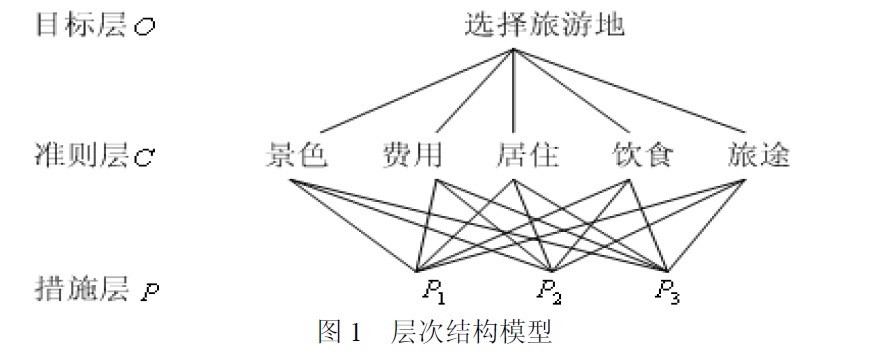
\includegraphics[scale=0.5]{Models/evaluation/AHP/Hierarchical model.png}
    \caption{Hierarchical model.}
    \label{fig:Hierarchical model}
\end{figure}

%%构造判断矩阵
(b)Construct the judgment matrix

(1)Construct the judgment matrix of $M-C$: Compare the elements of the criterion level in pairs to get the judgment matrix (see in Table \ref{tbl:Judgment matrix of O-C}).

\begin{table}[H]
    \renewcommand\arraystretch{2}   %%控制行间距
    \centering
    \begin{tabular}{llll}    %%三列均左对齐
        \toprule  %%表格横线加粗
        \specialrule{0em}{2pt}{2pt}    %%添加透明线控制行高
        $O$ & $C_1$ & $C_2$ & $C_3$ \\
        \specialrule{0em}{2pt}{2pt}    %%添加透明线控制行高
        \hline
        \specialrule{0em}{1pt}{1pt}    %%添加透明线控制行高
        $C_1$ & 1.0000 & 3.0000 & 4.0000 \\
        $C_2$ & 0.3333 & 1.0000 & 2.0000 \\
        $C_3$ & 0.2500 & 0.5000 & 1.0000 \\    
        \specialrule{0em}{1pt}{1pt}    %%添加透明线控制行高
        \bottomrule
    \end{tabular}
    \caption{Judgment matrix of $O-C$.}
    \label{tbl:Judgment matrix of O-C}
\end{table}

%%计算特征值，权重向量
%%代码见python
After that, it is easy to solve the eigenvalues of the matrix $M-C$ and the max eigenvalue is $\lambda_{max} = 3.0184$, thus getting the weight vector is $\omega_i = {(0.6250,0.2385,0.1365)}^T$.

Now we make the consistency check.

Since the consistency index $CI = \frac{\lambda_{max}-n}{n-1}$ and the consistency ratio $CR = \frac{CI}{RI}$, where $RI$ is only relative to the matrix size (see in Table \ref{tbl:The value of RI}).

By calculating, we get $CR = 0.0176<0.1$, which passes the consistency check.

%%The value of RI
\begin{table}[H]
    \renewcommand\arraystretch{2}   %%控制行间距
    \centering
    \begin{tabular}{ccccccccc}    %%三列均左对齐
        \toprule  %%表格横线加粗
        \specialrule{0em}{2pt}{2pt}    %%添加透明线控制行高
        matrix size & 2 & 3 & 4 & 5 & 6 & 7 & 8 & 9 \\
        \specialrule{0em}{2pt}{2pt}    %%添加透明线控制行高
        \hline
        \specialrule{0em}{1pt}{1pt}    %%添加透明线控制行高
        $RI$        & 0 & 0.58 & 0.90 & 1.12 & 1.24 & 1.32 & 1.41 & 1.45  \\
        \specialrule{0em}{1pt}{1pt}    %%添加透明线控制行高
        \bottomrule
    \end{tabular}
    \caption{The value of $RI$.}
    \label{tbl:The value of RI}
\end{table}

(2)Construct the judgment matrix of $C_1-P$, $C_2-P$ and $C_3-P$

Same as the formal part, we continue to construct the judgment matrix of $C_1-P$, $C_2-P$ and $C_3-P$ (see in Table \ref{tbl:Judgment matrix of C1-P}, \ref{tbl:Judgment matrix of C2-P} and \ref{tbl:Judgment matrix of C3-P})

\begin{table}[H]
    \renewcommand\arraystretch{2}   %%控制行间距
    \centering
    \begin{tabular}{llllll}    %%三列均左对齐
        \toprule  %%表格横线加粗
        \specialrule{0em}{2pt}{2pt}    %%添加透明线控制行高
        $C_1$ & $P_1$ & $P_2$ & $P_3$ & $P_4$ & $P_5$ \\
        \specialrule{0em}{2pt}{2pt}    %%添加透明线控制行高
        \hline
        \specialrule{0em}{1pt}{1pt}    %%添加透明线控制行高
        $P_1$ & 1.0000 & 3.0000 & 4.0000 & 1.0000 & 1.0000 \\
        $P_2$ & 0.3333 & 1.0000 & 2.0000 & 1.0000 & 1.0000 \\
        $P_3$ & 0.2500 & 0.5000 & 1.0000 & 1.0000 & 1.0000 \\
        $P_4$ & 1.0000 & 1.0000 & 1.0000 & 1.0000 & 1.0000 \\
        $P_5$ & 1.0000 & 1.0000 & 1.0000 & 1.0000 & 1.0000 \\
        \specialrule{0em}{1pt}{1pt}    %%添加透明线控制行高
        \bottomrule
    \end{tabular}
    \caption{Judgment matrix of $C_1-P$.}
    \label{tbl:Judgment matrix of C1-P}
\end{table}

\begin{table}[H]
    \renewcommand\arraystretch{2}   %%控制行间距
    \centering
    \begin{tabular}{lll}    %%三列均左对齐
        \toprule  %%表格横线加粗
        \specialrule{0em}{2pt}{2pt}    %%添加透明线控制行高
        $C_2$ & $P_6$ & $P_7$ \\
        \specialrule{0em}{2pt}{2pt}    %%添加透明线控制行高
        \hline
        \specialrule{0em}{1pt}{1pt}    %%添加透明线控制行高
        $P_6$ & 1.0000 & 3.0000 \\
        $P_7$ & 0.3333 & 1.0000 \\
        \specialrule{0em}{1pt}{1pt}    %%添加透明线控制行高
        \bottomrule
    \end{tabular}
    \caption{Judgment matrix of $C_2-P$.}
    \label{tbl:Judgment matrix of C2-P}
\end{table}

\begin{table}[H]
    \renewcommand\arraystretch{2}   %%控制行间距
    \centering
    \begin{tabular}{lll}    %%三列均左对齐
        \toprule  %%表格横线加粗
        \specialrule{0em}{2pt}{2pt}    %%添加透明线控制行高
        $C_3$ & $P_8$ & $P_9$ \\
        \specialrule{0em}{2pt}{2pt}    %%添加透明线控制行高
        \hline
        \specialrule{0em}{1pt}{1pt}    %%添加透明线控制行高
        $P_8$ & 1.0000 & 5.0000 \\
        $P_9$ & 0.2000 & 1.0000 \\
        \specialrule{0em}{1pt}{1pt}    %%添加透明线控制行高
        \bottomrule
    \end{tabular}
    \caption{Judgment matrix of $C_3-P$.}
    \label{tbl:Judgment matrix of C3-P}
\end{table}

By calculating, we get $CR_1 = 0.0785<0.1$, $CR_2 = 0.0000<0.1$, $CR_3 = 0.0000<0.1$, all of which pass the consistency check.

(c)model conclusion

From the formal four judgment matrices, we can calculate the total weights of each element in the plan level (see in table \ref{tbl:Element weights})

\begin{table}[H]
    \renewcommand\arraystretch{2}   %%控制行间距
    \centering
    \begin{tabular}{ll}    %%三列均左对齐
        \toprule  %%表格横线加粗
        \specialrule{0em}{2pt}{2pt}    %%添加透明线控制行高
        Evaluation index & Weight \\
        \specialrule{0em}{2pt}{2pt}    %%添加透明线控制行高
        \hline
        \specialrule{0em}{1pt}{1pt}    %%添加透明线控制行高
        $P_1$ & 0.1789 \\
        $P_2$ & 0.1594 \\
        $P_3$ & 0.1584 \\
        $P_4$ & 0.1535 \\
        $P_5$ & 0.1137 \\
        $P_6$ & 0.0906 \\
        $P_7$ & 0.0631 \\
        $P_8$ & 0.0596 \\
        $P_9$ & 0.0227 \\
        \specialrule{0em}{1pt}{1pt}    %%添加透明线控制行高
        \bottomrule
    \end{tabular}
    \caption{Element weights.}
    \label{tbl:Element weights}
\end{table}

Until now, we can set the whole index system of the evaluation of xxx (see in Figure \ref{fig:Index system}).

\begin{figure}[H]
    \centering
    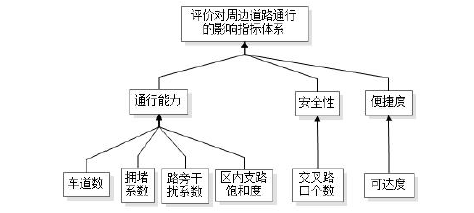
\includegraphics[scale=0.5]{Models/evaluation/AHP/Index system.png}
    \caption{Index system}
    \label{fig:Index system}
\end{figure}
% %%PCA
%%Principal Components Analysis 主成分分析法
%%Scree plot 碎石图

\subsection{PCA}

Here is a problem of the comprehensive evaluation of general higher education development level of different areas in China.

(a)Construct the comprehensive evaluation system

The introduction of the problem and set ten evaluation index in five aspects (see in Figure \ref{fig:Index system}).

%%评价指标图
\begin{figure}[H]
    \centering
    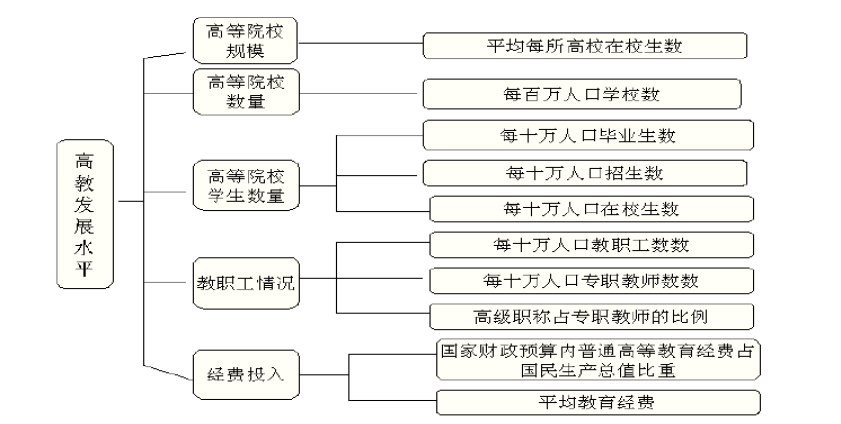
\includegraphics[scale=0.5]{Models/evaluation/PCA/Evaluation index.png}
    \caption{The ten evaluation index of higher education.}
    \label{fig:Evaluation index}
\end{figure}

(b)Data resources

Data source (see in Table \ref{tbl:Data of PCA}).

Define the ten indexes.

%%数据表格
\begin{table}[H]
    \renewcommand\arraystretch{2}   %%控制行间距
    \centering
    \begin{tabular}{|l|l|l|l|l|l|l|l|l|l|l|}    %%三列均左对齐
        \toprule  %%表格横线加粗
        \specialrule{0em}{2pt}{2pt}    %%添加透明线控制行高
        Area & $x_1$ & $x_2$ & $x_3$ & $x_4$ & $x_5$ & $x_6$ & $x_7$ & $x_8$ & $x_9$ & $x_{10}$ \\
        \specialrule{0em}{2pt}{2pt}    %%添加透明线控制行高
        \hline
        \specialrule{0em}{1pt}{1pt}    %%添加透明线控制行高
        Beijing & 5.96 & 310 & 461 & 1557 & 931 & 319 & 44.36 & 2615 & 2.20 & 13631 \\
        \hline
        Shanghai & 3.39 & 234 & 308 & 1035 & 498 & 161 & 35.02 & 3052 & 0.90 & 12665 \\
        \hline
        Tianjin & 2.35 & 157 & 229 & 713 & 295 & 109 & 38.40 & 3031 & 0.86 & 9385 \\
        \hline
        Shanxi & 1.35 & 81 & 111 & 364 & 150 & 58 & 30.45 & 2699 & 1.12 & 7881 \\
        \specialrule{0em}{1pt}{1pt}    %%添加透明线控制行高
        \bottomrule
    \end{tabular}
    \caption{Data of xxx.}
    \label{tbl:Data of PCA}
\end{table}

(c)Correlation analysis

From the data set, we can get the matrix of correlation coefficient (see in Table \ref{tbl:Matrix of PCA}).

\begin{table}[H]
    \renewcommand\arraystretch{2}   %%控制行间距
    \centering
    %% *{10}{r@{.}l|}重复10遍相同格式
    \begin{tabular}{|c|*{10}{r|}}    %%三列均左对齐
        \toprule  %%表格横线加粗
        \specialrule{0em}{2pt}{2pt}    %%添加透明线控制行高
         & $x_1$ & $x_2$ & $x_3$ & $x_4$ & $x_5$ & $x_6$ & $x_7$ & $x_8$ & $x_9$ & $x_{10}$ \\
        \specialrule{0em}{2pt}{2pt}    %%添加透明线控制行高
        \hline
        \specialrule{0em}{1pt}{1pt}    %%添加透明线控制行高
        $x_1$ & 1.000 & 0.963 & 0.984 & 0.987 & 0.999 & 1.000 & 0.892 & -0.378 & 0.801 & 0.906 \\
        \hline
        $x_2$ & 0.963 & 1.000 & 0.992 & 0.993 & 0.967 & 0.954 & 0.844 & -0.132 & 0.616 & 0.980 \\
        \hline
        $x_3$ & 0.984 & 0.992 & 1.000 & 0.999 & 0.984 & 0.978 & 0.896 & -0.208 & 0.682 & 0.949 \\
        \hline
        $x_4$ & 0.987 & 0.993 & 0.999 & 1.000 & 0.989 & 0.982 & 0.877 & -0.234 & 0.698 & 0.956 \\
        \hline
        $x_5$ & 0.999 & 0.967 & 0.984 & 0.989 & 1.000 & 0.998 & 0.869 & -0.376 & 0.795 & 0.920 \\
        \hline
        $x_6$ & 1.000 & 0.954 & 0.978 & 0.982 & 0.998 & 1.000 & 0.889 & -0.407 & 0.819 & 0.895 \\
        \hline
        $x_7$ & 0.892 & 0.844 & 0.896 & 0.887 & 0.869 & 0.889 & 1.000 & -0.225 & 0.668 & 0.720 \\
        \hline
        $x_8$ & -0.378 & -0.132 & -0.208 & -0.234 & -0.376 & -0.407 & -0.225 & 1.000 & -0.855 & -0.057 \\
        \hline
        $x_9$ & 0.801 & 0.616 & 0.682 & 0.698 & 0.795 & 0.819 & 0.668 & -0.855 & 1.000 & 0.524 \\
        \hline
        $x_{10}$ & 0.906 & 0.980 & 0.949 & 0.956 & 0.920 & 0.895 & 0.720 & -0.057 & 0.524 & 1.000 \\
        \specialrule{0em}{1pt}{1pt}    %%添加透明线控制行高
        \bottomrule
    \end{tabular}
    \caption{Matrix of correlation coefficient.}
    \label{tbl:Matrix of PCA}
\end{table}

\begin{figure}[H]
    \centering
    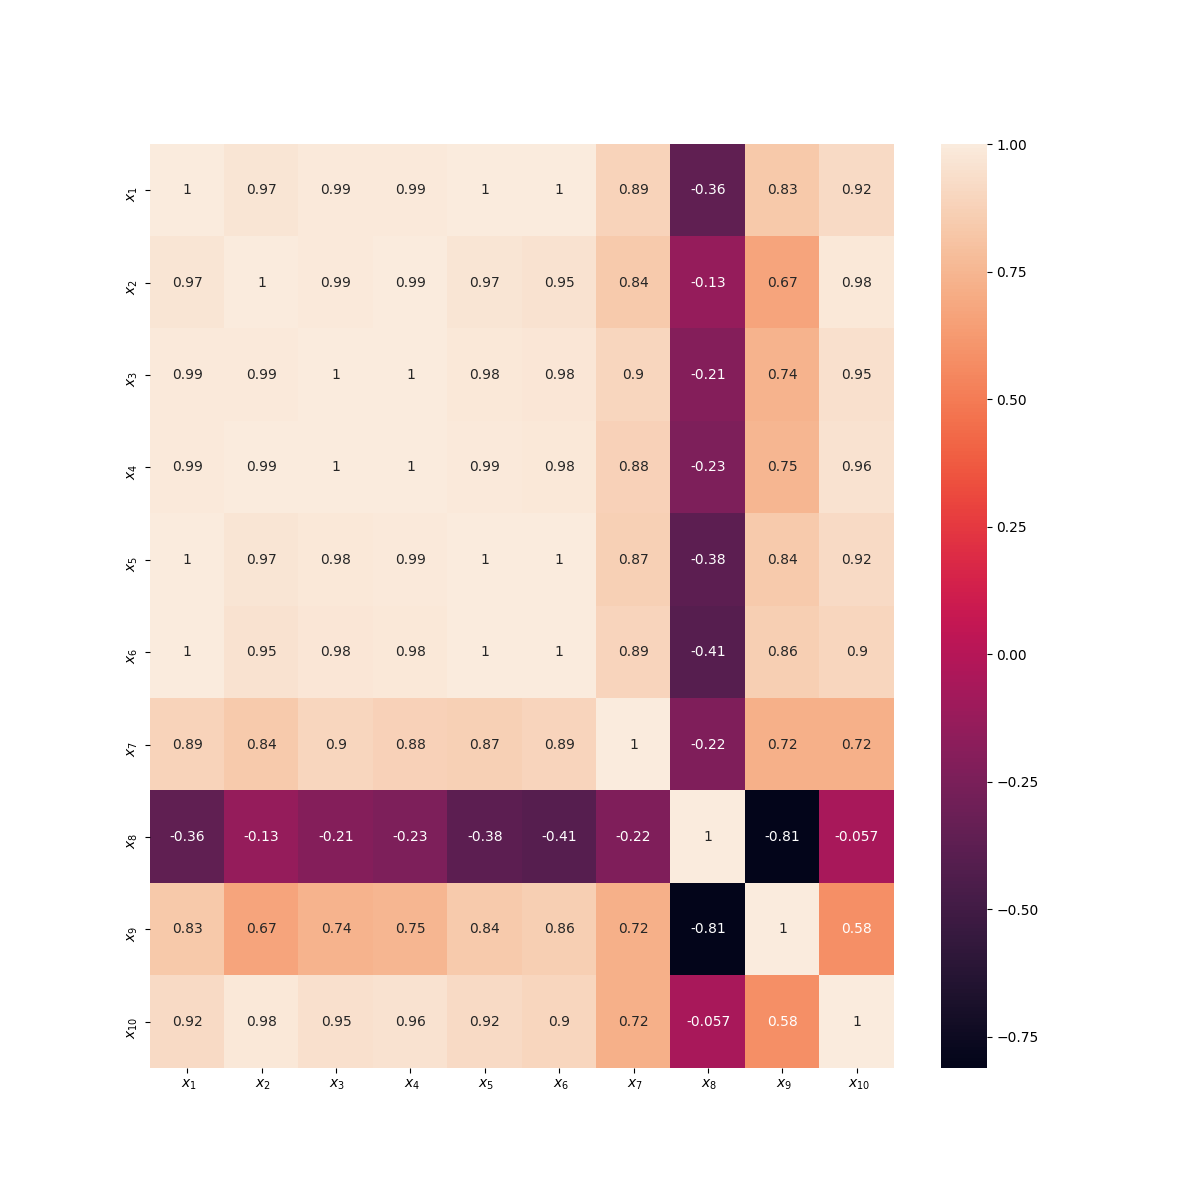
\includegraphics[width=5.5in]{Models/evaluation/PCA/PCA_correlation_analysis.png}
    \caption{PCA correlation analysis}
    \label{fig:PCA_correlation_analysis}
\end{figure}

We can see from the matrix that there exists strong correlation between some indexes. If we evaluate the problem directly, information overlap will occur, which affects the objectivity of the consequence.

(d)Conclusion

Then we use PCA to calculate eigenvalue and contribution rate (see in Table \ref{tbl:PCA consequence}).Also we can get the scree plot (see in Figure \ref{fig:Scree plot}).

\begin{table}[H]
    \renewcommand\arraystretch{2}   %%控制行间距
    \centering
    \begin{tabular}{|*{5}{r|}}    %%三列均左对齐
        \toprule  %%表格横线加粗
        \specialrule{0em}{2pt}{2pt}    %%添加透明线控制行高
        number & eigenvalue & contribution rate & cumulative contribution rate \\
        \specialrule{0em}{2pt}{2pt}    %%添加透明线控制行高
        \hline
        \specialrule{0em}{1pt}{1pt}    %%添加透明线控制行高
        1 & 8.269 & 82.690 & 82.690 \\
        \hline
        2 & 1.448 & 14.485 & 97.174 \\
        \hline
        3 & 0.283 & 2.826 & 100.000 \\
        \specialrule{0em}{1pt}{1pt}    %%添加透明线控制行高
        \bottomrule
    \end{tabular}
    \caption{PCA consequence.}
    \label{tbl:PCA consequence}
\end{table}

\begin{figure}[H]
    \centering
    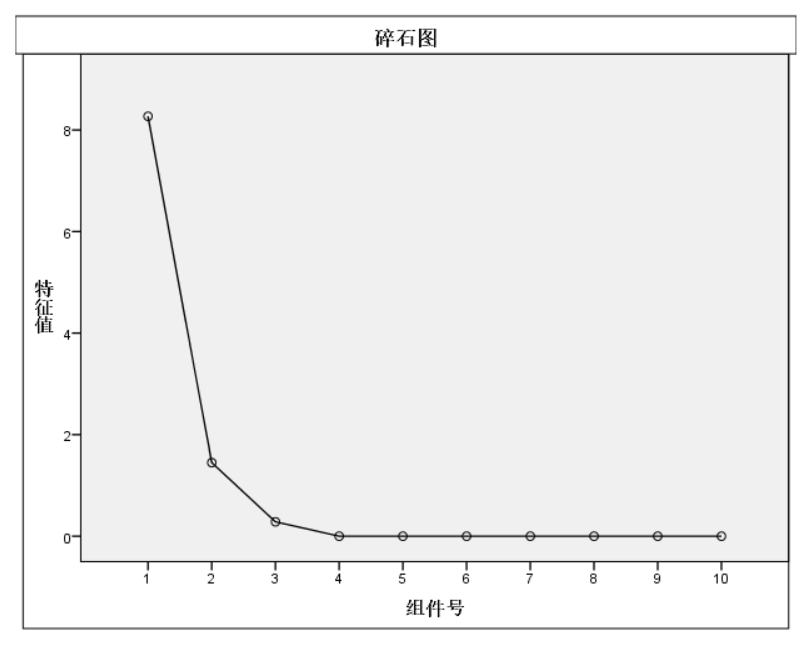
\includegraphics[scale=0.3]{Models/evaluation/PCA/Scree plot.png}
    \caption{Scree plot.}
    \label{fig:Scree plot}
\end{figure}

Through PCA, we can extract two principle components (see in Table \ref{tbl:Matrix of PCA components}).

\begin{table}[H]
    \renewcommand\arraystretch{2}   %%控制行间距
    \centering
    \begin{tabular}{|*{11}{r|}}    %%三列均左对齐
        \toprule  %%表格横线加粗
        \specialrule{0em}{2pt}{2pt}    %%添加透明线控制行高
        Component & $x_1$ & $x_2$ & $x_3$ & $x_4$ & $x_5$ & $x_6$ & $x_7$ & $x_8$ & $x_9$ & $x_{10}$ \\
        \specialrule{0em}{2pt}{2pt}    %%添加透明线控制行高
        \hline
        \specialrule{0em}{1pt}{1pt}    %%添加透明线控制行高
        1 & 1.000 & 0.966 & 0.987 & 0.990 & 0.999 & 0.999 & 0.892 & -0.365 & 0.792 & 0.912 \\
        \hline
        2 & -0.014 & 0.245 & 0.163 & 0.140 & -0.008 & -0.046 & 0.069 & 0.927 & -0.610 & 0.321 \\
        \specialrule{0em}{1pt}{1pt}    %%添加透明线控制行高
        \bottomrule
    \end{tabular}
    \caption{Matrix of components.}
    \label{tbl:Matrix of PCA components}
\end{table}

(e)Set the comprehensive evaluation system

From the coefficient of principle components, we can notice that xxx. (each component reflects which indexes)

Now, we take the contribution rare of the principle components as their ratio and get the comprehensive evaluation system.

\begin{equation*}
    Z = 0.8269y_1 + 0.1449y_2
\end{equation*}

And we get the score of the four areas (see in Table \ref{tbl:PCA score}).

\begin{table}[H]
    \renewcommand\arraystretch{2}   %%控制行间距
    \centering
    \begin{tabular}{|*{11}{r|}}    %%三列均左对齐
        \toprule  %%表格横线加粗
        \specialrule{0em}{2pt}{2pt}    %%添加透明线控制行高
        Area & Score \\
        \specialrule{0em}{2pt}{2pt}    %%添加透明线控制行高
        \hline
        \specialrule{0em}{1pt}{1pt}    %%添加透明线控制行高
        Beijing & 1.04 \\
        \hline
        Shanghai & 0.19 \\
        \hline
        Tianjin & -0.28 \\
        \hline
        Shanxi & -0.95 \\
        \specialrule{0em}{1pt}{1pt}    %%添加透明线控制行高
        \bottomrule
    \end{tabular}
    \caption{The score of the four areas.}
    \label{tbl:PCA score}
\end{table}
% %%TOPSIS
%%Technique for Order Preference by Similarity to an Ideal Solution
%%理想解法 优劣解距离法


\subsection{TOPSIS}
Here is problem of evaluating the water quality of 20 rivers.

\subsubsection{Data set}
Four indexes have been set and measured in the following table (see in Table \ref{tbl:TOPSIS-water quality data set}).
%%Data set table
%%三线表
\begin{table}[H]
    \renewcommand\arraystretch{2}   %%控制行间距
    \centering
    \begin{tabular}{c r@{.}l r@{.}l r@{.}l c}    %%各列对齐格式设置
        \toprule  %%表格横线加粗
        \specialrule{0em}{2pt}{2pt}    %%添加透明线控制行高
        \textbf{River}& \multicolumn{2}{l}{\textbf{Oxygen content}} & \multicolumn{2}{l}{\textbf{pH}} & \multicolumn{2}{l}{\textbf{Bacteria number}} & \textbf{Plant nutrients} \\
        \specialrule{0em}{2pt}{2pt}    %%添加透明线控制行高
        \midrule
        \specialrule{0em}{1pt}{1pt}
        1 & 4&69 & 6&59 & 51 & 11&94 \\
        2 & 2&03 & 7&86 & 19 & 6&46 \\
        3 & 9&11 & 6&31 & 46 & 8&91 \\
        4 & 8&61 & 7&05 & 46 & 26&43 \\
        5 & 7&13 & 6&50 & 50 & 23&57 \\
        6 & 2&39 & 6&77 & 38 & 24&62 \\
        7 & 7&69 & 6&79 & 38 & 6&01 \\
        8 & 9&30 & 6&81 & 27 & 31&57 \\
        9 & 5&45 & 7&62 & 5 & 18&46 \\
        10 & 6&19 & 7&27 & 17 & 7&51 \\
        11 & 7&93 & 7&53 & 9 & 6&52 \\
        12 & 4&40 & 7&28 & 17 & 25&30 \\
        13 & 7&46 & 8&24 & 23 & 14&42 \\
        14 & 2&01 & 5&55 & 47 & 26&31 \\
        15 & 2&04 & 6&40 & 23 & 17&91 \\
        16 & 7&73 & 6&14 & 52 & 15&72 \\
        17 & 6&35 & 7&58 & 25 & 29&46 \\ 
        18 & 8&29 & 8&41 & 39 & 12&02 \\
        19 & 3&54 & 7&27 & 54 & 3&16 \\
        20 & 7&44 & 6&26 & 8 & 28&41 \\
        \specialrule{0em}{1pt}{1pt}
        \bottomrule
    \end{tabular}
    \caption{TOPSIS-water quality data set.}
    \label{tbl:TOPSIS-water quality data set}
\end{table}


%%翻译不确定 极大型指标 极小型指标 中间型指标 区间型指标
\subsubsection{Data conversion}
In this part, the four indexes should be processed to 'very large index'.

(a)Oxygen content
High oxygen content indicates better water quality, so this index is a 'very large index', which doesn't need any processing.

(b)pH
Since the pH of water should be near 7, we have a 'middle index', and the best pH is 7.

To convert a 'middle index' to 'very large index', the following equation is applied here.

\begin{equation*}
    M = \max {|x_i-x_{best}|} , x_i' = 1 - \frac{|x_i-x_{best}|}{M}
\end{equation*}

(c)Bacteria number
The better the water quality is, the fewer the bacteria number should be. So the bacteria number is a 'very little index', which can be converted through the following way.

\begin{equation*}
    x_i' = max - x_i
\end{equation*}

(d)Plant nutrient
The index of the plant nutrient have an appropriate interval between 10 to 20, which should be converted to 'very large index' by using the following way.

In an 'interval index', $[a,b]$ is the stable interval and $[a^*,b^*]$ is the tolerant interval (the min and the max of data).

\begin{equation*}
    x' = \begin{cases}
    1 - \frac{a-x}{a-a*}, & x<a ; \\
    1 &, a \leq x \leq b ; \\
    1 - \frac{x-b}{b*-b}, & x>b .
    \end{cases}
\end{equation*}

\subsubsection{Construct the normalized initial matrix}
Then the normalized initial matrix can be constructed.

\subsubsection{Construct the index weight by AHP}

\subsubsection{Construct the evaluation system}

% \newpage
% \section{Correlation analysis}

% \newpage
% \section{Clustering analysis}
% %% LR
%% Logistic Regression 逻辑回归

\subsection{LR}

% 适用场景：对连续数据进行二分分类
% 例如：利用客户的个人信息和对某商品的打分和购买情况训练模型，筛选哪一类用户会购买该商品（文本评价可通过word2vec变成连续数据、高维数据可通过PCA降维，分类结果为购买/未购买）

(a) Map xxx into a two dimensional vector space

% PCA步骤

(b) Train the model

\begin{figure}[H]
    \centering
    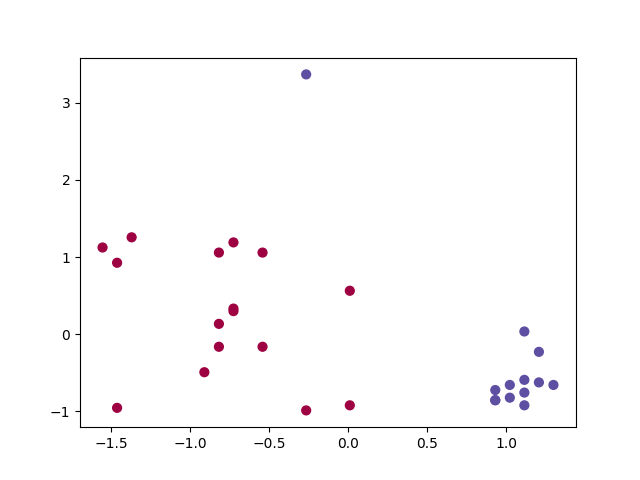
\includegraphics[width=\linewidth]{Models/clustering analysis/LR/LR_scatter.png}
    \caption{trained data}
    \label{fig:trained data}
\end{figure}

\begin{figure}[H]
    \centering
    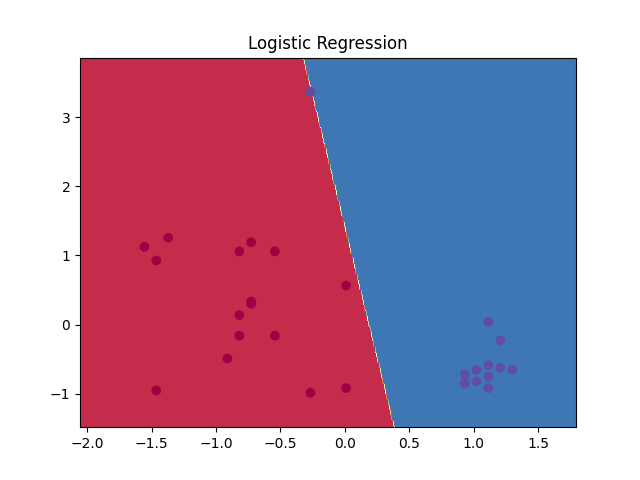
\includegraphics[width=\linewidth]{Models/clustering analysis/LR/LR.png}
    \caption{LR demo}
    \label{fig:LR_demo}
\end{figure}

(c) Predict with the model

% \newpage
% \section{Prediction}
% %%GM
%%Grey model 灰色预测

\subsection{GM}

\subsubsection{GM(1,1)}

%%设系统主变量原始数据序列为
\begin{displaymath}
X^{(0)}=(x^{(0)}(1),x^{(0)}(2),\ldots,x^{(0)}(m))
\end{displaymath}
%%其依次累加生成(Accumulating Generate Operator)序列为
\begin{displaymath}
X^{(1)}=(x^{(1)}(1),x^{(1)}(2),\ldots,x^{(1)}(m))
\end{displaymath}
%%其中
\begin{displaymath}
x^{(1)}(i)=\sum_{j=1}^{i}{x^{(0)}(j)}
\end{displaymath}
%%而序列
\begin{displaymath}
Z^{(1)}=(-,z^{(1)}(2),z^{(1)}(3),\ldots,z^{(1)}(m))
\end{displaymath}
%%被称为$X^{(1)}$的均值生成序列或系统的背景值，其中
\begin{displaymath}
z^{(1)}(i)=\frac{1}{2}(x^{(1)}(i)+x^{(1)}(i-1)),\qquad i=2,3,\ldots,m
\end{displaymath}
%%则称方程
\begin{displaymath}
x^{(0)}(i)+az^{(1)}(i)=b
\end{displaymath}
%%为一阶单变量灰色预测模型(One Order Single Variable Grey Model, $GM(1,1)$模型)。其中参数$a$是主变量参数或系统发展系数，$b$是$GM(1,1)$模型的灰作用系数或背景值。$\hat{a}=(a,b)^{T}$通过最小二乘方法取得，即设
\begin{displaymath}
Y=\left[
\begin{matrix}
x^{(0)}(2)\\
x^{(0)}(3)\\
\vdots\\
x^{(0)}(m)\\
\end{matrix}
\right]
\end{displaymath}

\begin{displaymath}
B=\left[
\begin{matrix}
-z^{(1)}(2) & 1 \\
-z^{(1)}(3) & 1 \\
\vdots & \vdots \\
-z^{(1)}(m) & 1 \\
\end{matrix}
\right]
\end{displaymath}
%%则
\begin{displaymath}
\hat{a}=(B^TB)^{-1}B^TY
\end{displaymath}
%%方程
\begin{displaymath}
\frac{\dif x^{(1)}}{\dif t}+ax^{(1)}=b
\end{displaymath}
%%被称为$GM(1,1)$模型的白化方程，也叫影子方程。结合$\hat{a}=(B^TB)^{-1}B^TY$所求解的$a,b$参数值，代入$\frac{dx^{(1)}}{dt}+ax^{(1)}=b$，可得$GM(1,1)$模型的时间响应序列为
\begin{displaymath}
\hat{x}^{(1)}(k+1)=(x^{(0)}(1)-\frac{b}{a})e^{-ak}+\frac{b}{a},\qquad k=2,3,\cdots,m-1
\end{displaymath}
%%通过上式可以求解依次累加生成序列$X^{(1)}$的模拟值$\hat{X}^{(1)}$，
\begin{displaymath}
\hat{X}^{(1)}=(\hat{x}^{(1)}(1),\hat{x}^{(1)}(2),\cdots,\hat{x}^{(1)}(m))
\end{displaymath}
%%运用方程
\begin{displaymath}
\hat{x}^{(0)}(k+1)=\hat{x}^{(1)}(k+1)-\hat{x}^{(1)}(k)
\end{displaymath}
%%可分别求解原始序列的模拟值和预测值$\hat{x}^{(0)}(k)$，排列所有$\hat{x}^{(0)}(k)$值可得原始序列的模拟值序列
\begin{displaymath}
\hat{X}^{(0)}=(\hat{x}^{(0)}(1),\hat{x}^{(0)}(2),\ldots,\hat{x}^{(0)}(m))
\end{displaymath}
%%结合$X^{(0)}=(x^{(0)}(1),x^{(0)}(2),\ldots,x^{(0)}(m))$和$\hat{X}^{(0)}=(\hat{x}^{(0)}(1),\hat{x}^{(0)}(2),\cdots,\hat{x}^{(0)}(m))$计算平均绝对误差(Mean Absolute Percent Error, MAPE)可得出模型仿真效果，MAPE被定义为
\begin{displaymath}
MAPE(\%)=\frac{1}{n}\sum_{k=1}^{n}|\frac{x^{(0)}(k)-\hat{x}^{(0)}(k)}{x^{(0)}(k)}|
\end{displaymath}
\par
%%对应上文所述灰色预测模型构建的一般分析过程，$GM(1,1)$模型的构建原理如下。\par
%%通常来说，如果输出数据$x^{(0)}(k)$适用于$GM(1,1)$，那么可以用MAPE来分析原始数据序列$X^{(0)}(k)$和模拟数据序列$\hat{X}^{(0)}(k)$之间的误差。事实上，$GM(1,1)$模型之所以是一个特殊灰色预测模型，只有主变量序列被考虑在模型的构建过程中，而不考虑任何其他影响因素。因此，$GM(1,1)$模型通常被用来研究系统主变量的自回归演化。从输入信息和输出结果来看，$GM(1,1)$模型的建模过程与其他时变预测模型相似。模拟序列的数据随着时间的变化而变化。不同的是，$GM(1,1)$模型构建是基于累加生成数据而其他时变预测模型基于原始序列。建模过程中，原始数据的随机扰动经过累加生成过程被大大减弱，使得系统增长规律得以涌现，即使当数据较少时，$GM(1,1)$模型仍然能够取得较好的模拟和预测效果。

\begin{figure}[H]
    \centering
    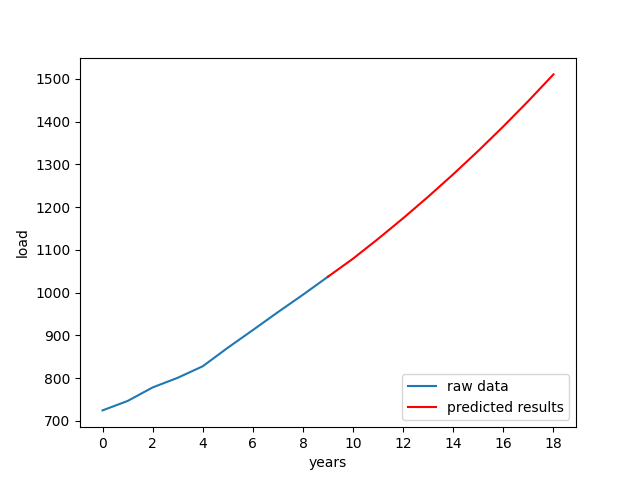
\includegraphics[width=\linewidth]{Models/prediction/GM/GM.png}
    \caption{prediction result}
    \label{fig:prediction result}
\end{figure}

% \newpage
% \section{Mathematical Formula}
In this section, Kualala is going to use latex to write some mathematical formulas and math symbols.

\subsection{Mathematical Formula-ex.1-symbol example}
Here is the Greek alphabet below, both lowercase and capital.
\begin{figure}[H]
    \centering
    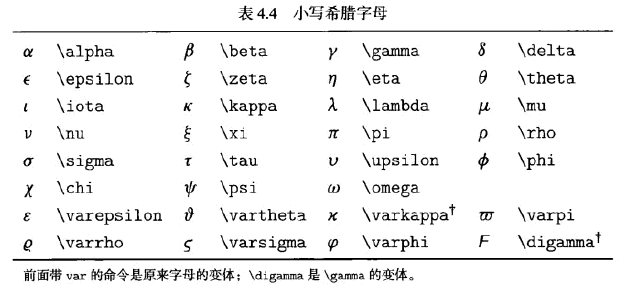
\includegraphics[scale=0.6]{Test/Test-formula/Greek-lowercase.png}
    \caption{Greek alphabet-lowercase.}
    \label{fig:Greek alphabet-lowercase}
\end{figure}

\begin{figure}[H]
    \centering
    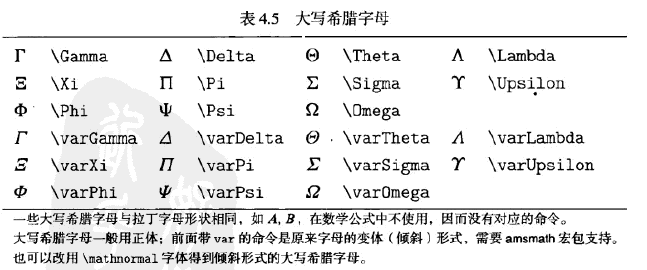
\includegraphics[scale=0.6]{Test/Test-formula/Greek-capital.png}
    \caption{Greek alphabet-capital.}
    \label{fig:Greek alphabet-capital}
\end{figure}

Here is some normal mathematical symbols.
\begin{figure}[H]
    \centering
    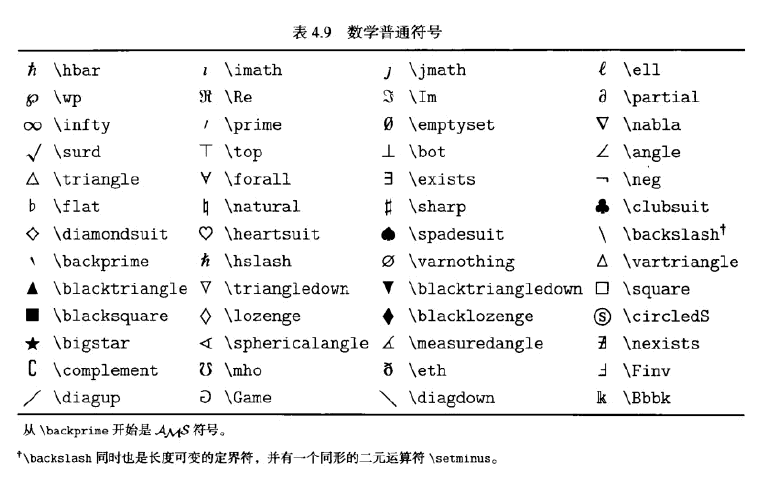
\includegraphics[scale=0.6]{Test/Test-formula/Normal symbols.png}
    \caption{Normal mathematical symbols.}
    \label{fig:Normal mathematical symbols.}
\end{figure}

Here is some relation symbol.
\begin{figure}[H]
    \centering
    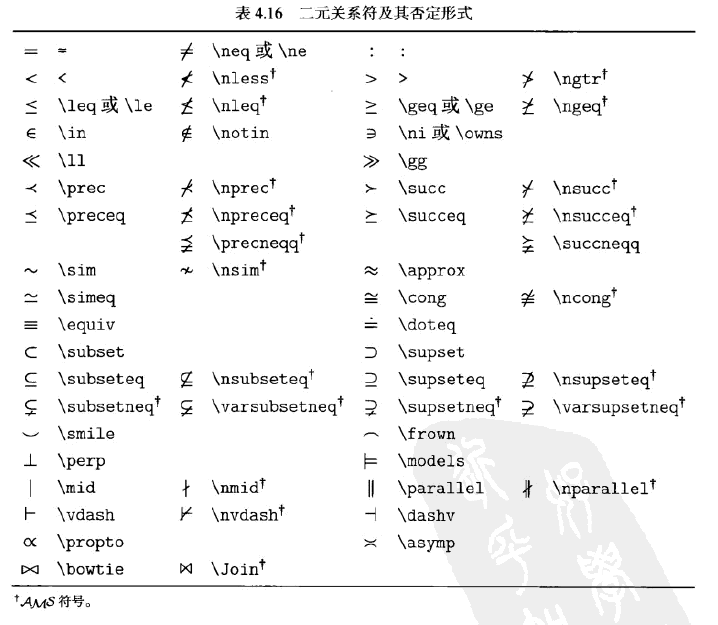
\includegraphics[scale=0.6]{Test/Test-formula/Relation symbols.png}
    \caption{Relation symbol.}
    \label{fig:Relation symbol}
\end{figure}

Here is other mathematical symbols.

$\dag$  \qquad  $\S$    \qquad  $\checkmark$

%%二项式系数
binomial coefficient:   \qquad
$\binom{2n}{n+1}$

\subsection{Mathematical Formula-ex.2-formula example}

$A_m^n$ \qquad  $A_m{}^n$   %%改变上标位置

$A_{ij} = 2^{i+j}$

$\overset{*}{X}$    \qquad
$\underset{*}{X}$   \qquad
$\overset{*}{\underset{\dag}{X}}$

Here we use tool to write a formula and give number to it.

Like for a sequence, see in Formula \ref{foumula:sequence}.

\begin{equation}
    K_{N_i} = K_{2^i} = 2^{N_i} = 2^{2^i}
    \label{foumula:sequence}
\end{equation}

Here are some examples below.

$3^{3^{3^{\cdot^{\cdot^{\cdot^3}}}}}$

$\angle A = 90^{\circ}$

%%sigma求和
$\max_n f(n) = \sum_{i=0}^n A_i$    \qquad
There is another writing way (or two more lines)
\[
    \max_n f(n) = \sum_{i=0}^n A_i
\]

%%sigma求和下标有两行
\[
    \sum_{\substack{0<i<n \\ 0<j<i}} A_{ij}
\]

%%prod求积
\[
    \sum_{i=0}^n A_i = \prod_{k=1}^m B_k
\]

%%积分
\[
    \int_0^1 f(t) \dif t = \iint_D g(x,y) \dif x \dif y
\]

%%求偏导
%%\left和\right可以转换为开符号和闭符号，并且自动调节大小
\[
    \partial_x \partial_y \left[
    \frac{1}{2} \left(x^2+y^2 \right)^2+xy
    \right]
\]

%%上下划线
$\overline{a+b} = \overline{a} + \overline{b}$, 
$\underline a = (a_0, a_1, a_2, \dots)$

%%上下箭头和花括号
$\overleftarrow{a+b}$, 
$\overleftrightarrow{a+b}$, 
$\overbrace{a+b+c}^{\text{$n+1$}} = \underbrace{1+2+3}$

\subsection{Mathematical Formula-ex.3-matrices}
Here are three kinds of matrices below.
%%圆括号矩阵
\[
    A = \begin{pmatrix}
            a_{11} & a_{12} & a_{13}    \\
            0 & a_{22} & a_{23}    \\
            0 & 0 & a_{33}
        \end{pmatrix}_{n\times n}
\]

%%方括号矩阵带矩阵大小
\[
    A = \begin{bmatrix}
            a_{11} & \dots & a_{in} \\
              & \ddots & \vdots  \\
            0 &  & a_{nn}
        \end{bmatrix}_{n\times n}
\]

%%矩阵元素位数不同对称，需要mathtools宏包
\[
    A = \begin{pmatrix*}[r]
            10 & -10 \\ -20 & 3
        \end{pmatrix*}_{2\times 2}
\]

\subsection{Mathematical Formula-ex.4-formulas more than one row}
Here is an example.
%%多行公式
\begin{gather}  %%编号环境
    a+b = b+a   \\
    ab = ba
\end{gather}

Here is another example.
\begin{gather*} %%不编号环境
    3+5 = 5+3 = 8   \\
    3\times 5 = 5\times 3
\end{gather*}

\begin{gather}
    3^2 + 4^2 = 5^2 \notag \\ %%手动不编号
    5^2 + 12^2 = 13^2 \notag \\ %%手动不编号
    a^2 + b^2 = c^2
\end{gather}    

\begin{align}
    x &= t + \cos t + 1 \\
    y &= 2 \sin t
\end{align}

\begin{align*}
    x &=t  & x &= \cos t    & x & = t \\
    y &=2t & y &= \sin(t+1) & y & = \sin t
\end{align*}

\begin{equation}
    \label{eq:dakuohao}
    D(x) = \begin{cases}
    1, & \text{if } x \in \mathbb{Q}; \\
    0, & \text{if } x \in \mathbb{R}\setminus\mathbb{Q}.
    \end{cases}
\end{equation}In this section, Kualala is going to use latex to write some mathematical formulas and math symbols.



\end{document}